\documentclass[12pt]{article}

\documentclass[12pt]{article}

\usepackage[utf8]{inputenc}
\usepackage[english]{babel}

\usepackage{amssymb, mathtools, amsmath, amsthm}
\usepackage[italicdiff]{physics}

\usepackage[none]{hyphenat}             % disables hyphenated words at end of paragraph
%\setlength{\parindent}{0pt}             % removes paragraph indent
%\setlength{\parskip}{11pt}              % adds space between paragraphs

\usepackage{geometry}
\newlength{\alphabet}
\settowidth{\alphabet}{abcdefghijklmnopqrstuvwxyz}
\geometry{textwidth=2.5\alphabet}

\usepackage{enumitem}
\setlist[enumerate,1]{leftmargin=0pt}   % pushes enum items to the margin

%\usepackage{libertine}
%\usepackage[libertine, vvarbb]{newtxmath}

\usepackage[space]{erewhon}             % font
\usepackage[erewhon, vvarbb]{newtxmath} % math font

%\usepackage[scale=0.90]{tgheros}        % sans serif
%\usepackage[scale=0.90,lf]{FiraMono}    % monospace
\usepackage[T1]{fontenc}
\usepackage{microtype}


\newcommand{\C}{\mathbf C}
\newcommand{\F}{\mathbf F}
\newcommand{\N}{\mathbf N}
\newcommand{\PP}{\textbf P}
\newcommand{\Q}{\mathbf Q}
\newcommand{\R}{\mathbf R}
\newcommand{\Z}{\mathbf Z}

\newcommand{\inv}{^{-1}}
\newcommand{\eps}{\varepsilon}

\DeclareMathOperator{\Aut}{Aut}
\DeclareMathOperator{\Char}{char}
\DeclareMathOperator{\End}{End}
\DeclareMathOperator{\Gal}{Gal}
\DeclareMathOperator{\GL}{GL}
\DeclareMathOperator{\Hom}{Hom}
\DeclareMathOperator{\Ind}{Ind}
\DeclareMathOperator{\SL}{SL}
\DeclareMathOperator{\Spec}{Spec}

\DeclareMathOperator{\coker}{coker}
\DeclareMathOperator{\im}{im}

\newtheorem{theorem}{Theorem}
\newtheorem{lemma}[theorem]{Lemma}

\theoremstyle{definition}
\newtheorem{definition}[theorem]{Definition}

\newtheorem*{example}{Example}


\usepackage{tikz}

\title{Elementary}
\author{}
\date{}

\begin{document}

\maketitle
\tableofcontents

\newpage

\section{Operations}

\subsection{Addition}

\subsection{Multiplication}

Multiplication is just counting by groups.
You can count to 15 one by one, or you can count 5 groups of 3, or 3 groups of 5.
The expression \( ab \)
is the quantity you get when you take \( a \) units and make \( b \) groups of it.

\tikzset{every picture/.style={line width=0.75pt}} %set default line width to 0.75pt        

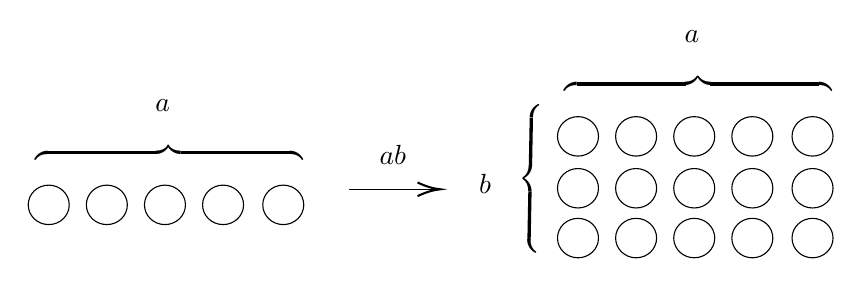
\begin{tikzpicture}[x=0.75pt,y=0.75pt,yscale=-1,xscale=1]
%uncomment if require: \path (0,300); %set diagram left start at 0, and has height of 300

%Shape: Ellipse [id:dp01701625434648868] 
\draw   (130,150.5) .. controls (130,145.25) and (134.42,141) .. (139.88,141) .. controls (145.33,141) and (149.75,145.25) .. (149.75,150.5) .. controls (149.75,155.75) and (145.33,160) .. (139.88,160) .. controls (134.42,160) and (130,155.75) .. (130,150.5) -- cycle ;
%Shape: Ellipse [id:dp5911952995920767] 
\draw   (158,150.5) .. controls (158,145.25) and (162.42,141) .. (167.88,141) .. controls (173.33,141) and (177.75,145.25) .. (177.75,150.5) .. controls (177.75,155.75) and (173.33,160) .. (167.88,160) .. controls (162.42,160) and (158,155.75) .. (158,150.5) -- cycle ;
%Shape: Ellipse [id:dp12827961502607044] 
\draw   (186,150.5) .. controls (186,145.25) and (190.42,141) .. (195.88,141) .. controls (201.33,141) and (205.75,145.25) .. (205.75,150.5) .. controls (205.75,155.75) and (201.33,160) .. (195.88,160) .. controls (190.42,160) and (186,155.75) .. (186,150.5) -- cycle ;
%Shape: Ellipse [id:dp17486866021427894] 
\draw   (214,150.5) .. controls (214,145.25) and (218.42,141) .. (223.88,141) .. controls (229.33,141) and (233.75,145.25) .. (233.75,150.5) .. controls (233.75,155.75) and (229.33,160) .. (223.88,160) .. controls (218.42,160) and (214,155.75) .. (214,150.5) -- cycle ;
%Shape: Ellipse [id:dp5769227894290598] 
\draw   (243,150.5) .. controls (243,145.25) and (247.42,141) .. (252.88,141) .. controls (258.33,141) and (262.75,145.25) .. (262.75,150.5) .. controls (262.75,155.75) and (258.33,160) .. (252.88,160) .. controls (247.42,160) and (243,155.75) .. (243,150.5) -- cycle ;
%Straight Lines [id:da8686391579148476] 
\draw    (284.5,143) -- (326.5,143) ;
\draw [shift={(328.5,143)}, rotate = 180] [color={rgb, 255:red, 0; green, 0; blue, 0 }  ][line width=0.75]    (10.93,-3.29) .. controls (6.95,-1.4) and (3.31,-0.3) .. (0,0) .. controls (3.31,0.3) and (6.95,1.4) .. (10.93,3.29)   ;
%Shape: Ellipse [id:dp25092936651447906] 
\draw   (385,117.5) .. controls (385,112.25) and (389.42,108) .. (394.88,108) .. controls (400.33,108) and (404.75,112.25) .. (404.75,117.5) .. controls (404.75,122.75) and (400.33,127) .. (394.88,127) .. controls (389.42,127) and (385,122.75) .. (385,117.5) -- cycle ;
%Shape: Ellipse [id:dp0966701654609392] 
\draw   (413,117.5) .. controls (413,112.25) and (417.42,108) .. (422.88,108) .. controls (428.33,108) and (432.75,112.25) .. (432.75,117.5) .. controls (432.75,122.75) and (428.33,127) .. (422.88,127) .. controls (417.42,127) and (413,122.75) .. (413,117.5) -- cycle ;
%Shape: Ellipse [id:dp0766023058181281] 
\draw   (441,117.5) .. controls (441,112.25) and (445.42,108) .. (450.88,108) .. controls (456.33,108) and (460.75,112.25) .. (460.75,117.5) .. controls (460.75,122.75) and (456.33,127) .. (450.88,127) .. controls (445.42,127) and (441,122.75) .. (441,117.5) -- cycle ;
%Shape: Ellipse [id:dp836829648867243] 
\draw   (469,117.5) .. controls (469,112.25) and (473.42,108) .. (478.88,108) .. controls (484.33,108) and (488.75,112.25) .. (488.75,117.5) .. controls (488.75,122.75) and (484.33,127) .. (478.88,127) .. controls (473.42,127) and (469,122.75) .. (469,117.5) -- cycle ;
%Shape: Ellipse [id:dp501644978386966] 
\draw   (498,117.5) .. controls (498,112.25) and (502.42,108) .. (507.88,108) .. controls (513.33,108) and (517.75,112.25) .. (517.75,117.5) .. controls (517.75,122.75) and (513.33,127) .. (507.88,127) .. controls (502.42,127) and (498,122.75) .. (498,117.5) -- cycle ;
%Shape: Ellipse [id:dp7146236362007783] 
\draw   (385,142.5) .. controls (385,137.25) and (389.42,133) .. (394.88,133) .. controls (400.33,133) and (404.75,137.25) .. (404.75,142.5) .. controls (404.75,147.75) and (400.33,152) .. (394.88,152) .. controls (389.42,152) and (385,147.75) .. (385,142.5) -- cycle ;
%Shape: Ellipse [id:dp2533805495129937] 
\draw   (413,142.5) .. controls (413,137.25) and (417.42,133) .. (422.88,133) .. controls (428.33,133) and (432.75,137.25) .. (432.75,142.5) .. controls (432.75,147.75) and (428.33,152) .. (422.88,152) .. controls (417.42,152) and (413,147.75) .. (413,142.5) -- cycle ;
%Shape: Ellipse [id:dp4880802746789624] 
\draw   (441,142.5) .. controls (441,137.25) and (445.42,133) .. (450.88,133) .. controls (456.33,133) and (460.75,137.25) .. (460.75,142.5) .. controls (460.75,147.75) and (456.33,152) .. (450.88,152) .. controls (445.42,152) and (441,147.75) .. (441,142.5) -- cycle ;
%Shape: Ellipse [id:dp13535591876302167] 
\draw   (469,142.5) .. controls (469,137.25) and (473.42,133) .. (478.88,133) .. controls (484.33,133) and (488.75,137.25) .. (488.75,142.5) .. controls (488.75,147.75) and (484.33,152) .. (478.88,152) .. controls (473.42,152) and (469,147.75) .. (469,142.5) -- cycle ;
%Shape: Ellipse [id:dp24334690544668647] 
\draw   (498,142.5) .. controls (498,137.25) and (502.42,133) .. (507.88,133) .. controls (513.33,133) and (517.75,137.25) .. (517.75,142.5) .. controls (517.75,147.75) and (513.33,152) .. (507.88,152) .. controls (502.42,152) and (498,147.75) .. (498,142.5) -- cycle ;
%Shape: Ellipse [id:dp9272226675640204] 
\draw   (385,166.5) .. controls (385,161.25) and (389.42,157) .. (394.88,157) .. controls (400.33,157) and (404.75,161.25) .. (404.75,166.5) .. controls (404.75,171.75) and (400.33,176) .. (394.88,176) .. controls (389.42,176) and (385,171.75) .. (385,166.5) -- cycle ;
%Shape: Ellipse [id:dp4548669959652437] 
\draw   (413,166.5) .. controls (413,161.25) and (417.42,157) .. (422.88,157) .. controls (428.33,157) and (432.75,161.25) .. (432.75,166.5) .. controls (432.75,171.75) and (428.33,176) .. (422.88,176) .. controls (417.42,176) and (413,171.75) .. (413,166.5) -- cycle ;
%Shape: Ellipse [id:dp0793974201297154] 
\draw   (441,166.5) .. controls (441,161.25) and (445.42,157) .. (450.88,157) .. controls (456.33,157) and (460.75,161.25) .. (460.75,166.5) .. controls (460.75,171.75) and (456.33,176) .. (450.88,176) .. controls (445.42,176) and (441,171.75) .. (441,166.5) -- cycle ;
%Shape: Ellipse [id:dp6099965284805888] 
\draw   (469,166.5) .. controls (469,161.25) and (473.42,157) .. (478.88,157) .. controls (484.33,157) and (488.75,161.25) .. (488.75,166.5) .. controls (488.75,171.75) and (484.33,176) .. (478.88,176) .. controls (473.42,176) and (469,171.75) .. (469,166.5) -- cycle ;
%Shape: Ellipse [id:dp3818995158485563] 
\draw   (498,166.5) .. controls (498,161.25) and (502.42,157) .. (507.88,157) .. controls (513.33,157) and (517.75,161.25) .. (517.75,166.5) .. controls (517.75,171.75) and (513.33,176) .. (507.88,176) .. controls (502.42,176) and (498,171.75) .. (498,166.5) -- cycle ;

% Text Node
\draw (190,98.4) node [anchor=north west][inner sep=0.75pt]    {$a$};
% Text Node
\draw (132,120.4) node [anchor=north west][inner sep=0.75pt]    {$\overbrace{\ \ \ \ \ \ \ \ \ \ \ \ \ \ \ \ \ \ \ \ \ \ \ \ \ \ \ \ \ }$};
% Text Node
\draw (445,65.4) node [anchor=north west][inner sep=0.75pt]    {$a$};
% Text Node
\draw (387,87.4) node [anchor=north west][inner sep=0.75pt]    {$\overbrace{\ \ \ \ \ \ \ \ \ \ \ \ \ \ \ \ \ \ \ \ \ \ \ \ \ \ \ \ \ }$};
% Text Node
\draw (366.21,174.74) node [anchor=north west][inner sep=0.75pt]  [rotate=-271.09]  {$\overbrace{\ \ \ \ \ \ \ \ \ \ \ \ \ \ \ \ }$};
% Text Node
\draw (346,134.4) node [anchor=north west][inner sep=0.75pt]    {$b$};
% Text Node
\draw (298,120.4) node [anchor=north west][inner sep=0.75pt]    {$ab$};


\end{tikzpicture}

We can take the groups in any order we like, so multiplication is commutative:
\( ab = ba \).

\tikzset{every picture/.style={line width=0.75pt}} %set default line width to 0.75pt        

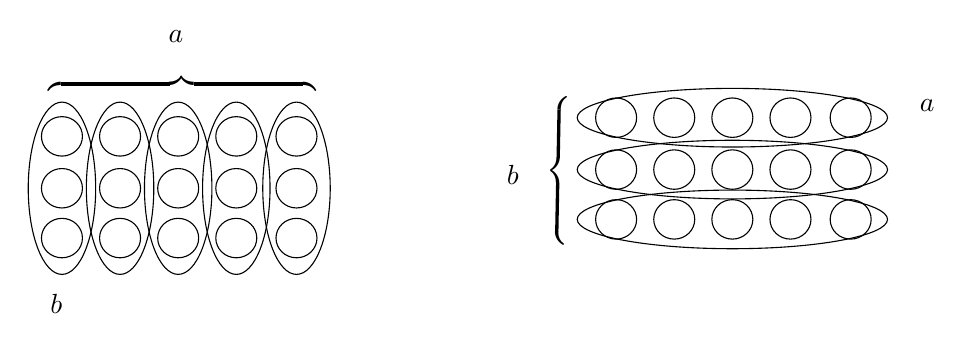
\begin{tikzpicture}[x=0.75pt,y=0.75pt,yscale=-1,xscale=1]
%uncomment if require: \path (0,300); %set diagram left start at 0, and has height of 300

%Shape: Ellipse [id:dp9022669979434795] 
\draw   (128,118.5) .. controls (128,113.25) and (132.42,109) .. (137.88,109) .. controls (143.33,109) and (147.75,113.25) .. (147.75,118.5) .. controls (147.75,123.75) and (143.33,128) .. (137.88,128) .. controls (132.42,128) and (128,123.75) .. (128,118.5) -- cycle ;
%Shape: Ellipse [id:dp1393703351282003] 
\draw   (156,118.5) .. controls (156,113.25) and (160.42,109) .. (165.88,109) .. controls (171.33,109) and (175.75,113.25) .. (175.75,118.5) .. controls (175.75,123.75) and (171.33,128) .. (165.88,128) .. controls (160.42,128) and (156,123.75) .. (156,118.5) -- cycle ;
%Shape: Ellipse [id:dp32808292902806224] 
\draw   (184,118.5) .. controls (184,113.25) and (188.42,109) .. (193.88,109) .. controls (199.33,109) and (203.75,113.25) .. (203.75,118.5) .. controls (203.75,123.75) and (199.33,128) .. (193.88,128) .. controls (188.42,128) and (184,123.75) .. (184,118.5) -- cycle ;
%Shape: Ellipse [id:dp9820585267166347] 
\draw   (212,118.5) .. controls (212,113.25) and (216.42,109) .. (221.88,109) .. controls (227.33,109) and (231.75,113.25) .. (231.75,118.5) .. controls (231.75,123.75) and (227.33,128) .. (221.88,128) .. controls (216.42,128) and (212,123.75) .. (212,118.5) -- cycle ;
%Shape: Ellipse [id:dp6155422737978968] 
\draw   (241,118.5) .. controls (241,113.25) and (245.42,109) .. (250.88,109) .. controls (256.33,109) and (260.75,113.25) .. (260.75,118.5) .. controls (260.75,123.75) and (256.33,128) .. (250.88,128) .. controls (245.42,128) and (241,123.75) .. (241,118.5) -- cycle ;
%Shape: Ellipse [id:dp6403408502350825] 
\draw   (128,143.5) .. controls (128,138.25) and (132.42,134) .. (137.88,134) .. controls (143.33,134) and (147.75,138.25) .. (147.75,143.5) .. controls (147.75,148.75) and (143.33,153) .. (137.88,153) .. controls (132.42,153) and (128,148.75) .. (128,143.5) -- cycle ;
%Shape: Ellipse [id:dp6795726159570024] 
\draw   (156,143.5) .. controls (156,138.25) and (160.42,134) .. (165.88,134) .. controls (171.33,134) and (175.75,138.25) .. (175.75,143.5) .. controls (175.75,148.75) and (171.33,153) .. (165.88,153) .. controls (160.42,153) and (156,148.75) .. (156,143.5) -- cycle ;
%Shape: Ellipse [id:dp1655530263189846] 
\draw   (184,143.5) .. controls (184,138.25) and (188.42,134) .. (193.88,134) .. controls (199.33,134) and (203.75,138.25) .. (203.75,143.5) .. controls (203.75,148.75) and (199.33,153) .. (193.88,153) .. controls (188.42,153) and (184,148.75) .. (184,143.5) -- cycle ;
%Shape: Ellipse [id:dp5826904027150761] 
\draw   (212,143.5) .. controls (212,138.25) and (216.42,134) .. (221.88,134) .. controls (227.33,134) and (231.75,138.25) .. (231.75,143.5) .. controls (231.75,148.75) and (227.33,153) .. (221.88,153) .. controls (216.42,153) and (212,148.75) .. (212,143.5) -- cycle ;
%Shape: Ellipse [id:dp8484023027634976] 
\draw   (241,143.5) .. controls (241,138.25) and (245.42,134) .. (250.88,134) .. controls (256.33,134) and (260.75,138.25) .. (260.75,143.5) .. controls (260.75,148.75) and (256.33,153) .. (250.88,153) .. controls (245.42,153) and (241,148.75) .. (241,143.5) -- cycle ;
%Shape: Ellipse [id:dp6331710262737843] 
\draw   (128,167.5) .. controls (128,162.25) and (132.42,158) .. (137.88,158) .. controls (143.33,158) and (147.75,162.25) .. (147.75,167.5) .. controls (147.75,172.75) and (143.33,177) .. (137.88,177) .. controls (132.42,177) and (128,172.75) .. (128,167.5) -- cycle ;
%Shape: Ellipse [id:dp19986717409631727] 
\draw   (156,167.5) .. controls (156,162.25) and (160.42,158) .. (165.88,158) .. controls (171.33,158) and (175.75,162.25) .. (175.75,167.5) .. controls (175.75,172.75) and (171.33,177) .. (165.88,177) .. controls (160.42,177) and (156,172.75) .. (156,167.5) -- cycle ;
%Shape: Ellipse [id:dp16352783760247158] 
\draw   (184,167.5) .. controls (184,162.25) and (188.42,158) .. (193.88,158) .. controls (199.33,158) and (203.75,162.25) .. (203.75,167.5) .. controls (203.75,172.75) and (199.33,177) .. (193.88,177) .. controls (188.42,177) and (184,172.75) .. (184,167.5) -- cycle ;
%Shape: Ellipse [id:dp3282999501414655] 
\draw   (212,167.5) .. controls (212,162.25) and (216.42,158) .. (221.88,158) .. controls (227.33,158) and (231.75,162.25) .. (231.75,167.5) .. controls (231.75,172.75) and (227.33,177) .. (221.88,177) .. controls (216.42,177) and (212,172.75) .. (212,167.5) -- cycle ;
%Shape: Ellipse [id:dp08662024231560805] 
\draw   (241,167.5) .. controls (241,162.25) and (245.42,158) .. (250.88,158) .. controls (256.33,158) and (260.75,162.25) .. (260.75,167.5) .. controls (260.75,172.75) and (256.33,177) .. (250.88,177) .. controls (245.42,177) and (241,172.75) .. (241,167.5) -- cycle ;
%Shape: Ellipse [id:dp3735495223162667] 
\draw   (121.63,143.5) .. controls (121.63,120.58) and (128.9,102) .. (137.88,102) .. controls (146.85,102) and (154.13,120.58) .. (154.13,143.5) .. controls (154.13,166.42) and (146.85,185) .. (137.88,185) .. controls (128.9,185) and (121.63,166.42) .. (121.63,143.5) -- cycle ;
%Shape: Ellipse [id:dp5565298752337068] 
\draw   (149.63,143.5) .. controls (149.63,120.58) and (156.9,102) .. (165.88,102) .. controls (174.85,102) and (182.13,120.58) .. (182.13,143.5) .. controls (182.13,166.42) and (174.85,185) .. (165.88,185) .. controls (156.9,185) and (149.63,166.42) .. (149.63,143.5) -- cycle ;
%Shape: Ellipse [id:dp35183898993696516] 
\draw   (177.63,143.5) .. controls (177.63,120.58) and (184.9,102) .. (193.88,102) .. controls (202.85,102) and (210.13,120.58) .. (210.13,143.5) .. controls (210.13,166.42) and (202.85,185) .. (193.88,185) .. controls (184.9,185) and (177.63,166.42) .. (177.63,143.5) -- cycle ;
%Shape: Ellipse [id:dp15461155750615496] 
\draw   (205.63,143.5) .. controls (205.63,120.58) and (212.9,102) .. (221.88,102) .. controls (230.85,102) and (238.13,120.58) .. (238.13,143.5) .. controls (238.13,166.42) and (230.85,185) .. (221.88,185) .. controls (212.9,185) and (205.63,166.42) .. (205.63,143.5) -- cycle ;
%Shape: Ellipse [id:dp9451740281118809] 
\draw   (234.63,143.5) .. controls (234.63,120.58) and (241.9,102) .. (250.88,102) .. controls (259.85,102) and (267.13,120.58) .. (267.13,143.5) .. controls (267.13,166.42) and (259.85,185) .. (250.88,185) .. controls (241.9,185) and (234.63,166.42) .. (234.63,143.5) -- cycle ;
%Shape: Ellipse [id:dp40403708195800314] 
\draw   (395,109.5) .. controls (395,104.25) and (399.42,100) .. (404.88,100) .. controls (410.33,100) and (414.75,104.25) .. (414.75,109.5) .. controls (414.75,114.75) and (410.33,119) .. (404.88,119) .. controls (399.42,119) and (395,114.75) .. (395,109.5) -- cycle ;
%Shape: Ellipse [id:dp4102344211942396] 
\draw   (423,109.5) .. controls (423,104.25) and (427.42,100) .. (432.88,100) .. controls (438.33,100) and (442.75,104.25) .. (442.75,109.5) .. controls (442.75,114.75) and (438.33,119) .. (432.88,119) .. controls (427.42,119) and (423,114.75) .. (423,109.5) -- cycle ;
%Shape: Ellipse [id:dp5445437061677258] 
\draw   (451,109.5) .. controls (451,104.25) and (455.42,100) .. (460.88,100) .. controls (466.33,100) and (470.75,104.25) .. (470.75,109.5) .. controls (470.75,114.75) and (466.33,119) .. (460.88,119) .. controls (455.42,119) and (451,114.75) .. (451,109.5) -- cycle ;
%Shape: Ellipse [id:dp3817547397810592] 
\draw   (479,109.5) .. controls (479,104.25) and (483.42,100) .. (488.88,100) .. controls (494.33,100) and (498.75,104.25) .. (498.75,109.5) .. controls (498.75,114.75) and (494.33,119) .. (488.88,119) .. controls (483.42,119) and (479,114.75) .. (479,109.5) -- cycle ;
%Shape: Ellipse [id:dp03174413367735651] 
\draw   (508,109.5) .. controls (508,104.25) and (512.42,100) .. (517.88,100) .. controls (523.33,100) and (527.75,104.25) .. (527.75,109.5) .. controls (527.75,114.75) and (523.33,119) .. (517.88,119) .. controls (512.42,119) and (508,114.75) .. (508,109.5) -- cycle ;
%Shape: Ellipse [id:dp46727249724573305] 
\draw   (395,134.5) .. controls (395,129.25) and (399.42,125) .. (404.88,125) .. controls (410.33,125) and (414.75,129.25) .. (414.75,134.5) .. controls (414.75,139.75) and (410.33,144) .. (404.88,144) .. controls (399.42,144) and (395,139.75) .. (395,134.5) -- cycle ;
%Shape: Ellipse [id:dp2836269316726524] 
\draw   (423,134.5) .. controls (423,129.25) and (427.42,125) .. (432.88,125) .. controls (438.33,125) and (442.75,129.25) .. (442.75,134.5) .. controls (442.75,139.75) and (438.33,144) .. (432.88,144) .. controls (427.42,144) and (423,139.75) .. (423,134.5) -- cycle ;
%Shape: Ellipse [id:dp37957946852436375] 
\draw   (451,134.5) .. controls (451,129.25) and (455.42,125) .. (460.88,125) .. controls (466.33,125) and (470.75,129.25) .. (470.75,134.5) .. controls (470.75,139.75) and (466.33,144) .. (460.88,144) .. controls (455.42,144) and (451,139.75) .. (451,134.5) -- cycle ;
%Shape: Ellipse [id:dp1943038380866695] 
\draw   (479,134.5) .. controls (479,129.25) and (483.42,125) .. (488.88,125) .. controls (494.33,125) and (498.75,129.25) .. (498.75,134.5) .. controls (498.75,139.75) and (494.33,144) .. (488.88,144) .. controls (483.42,144) and (479,139.75) .. (479,134.5) -- cycle ;
%Shape: Ellipse [id:dp9241785241521442] 
\draw   (508,134.5) .. controls (508,129.25) and (512.42,125) .. (517.88,125) .. controls (523.33,125) and (527.75,129.25) .. (527.75,134.5) .. controls (527.75,139.75) and (523.33,144) .. (517.88,144) .. controls (512.42,144) and (508,139.75) .. (508,134.5) -- cycle ;
%Shape: Ellipse [id:dp990167094985511] 
\draw   (395,158.5) .. controls (395,153.25) and (399.42,149) .. (404.88,149) .. controls (410.33,149) and (414.75,153.25) .. (414.75,158.5) .. controls (414.75,163.75) and (410.33,168) .. (404.88,168) .. controls (399.42,168) and (395,163.75) .. (395,158.5) -- cycle ;
%Shape: Ellipse [id:dp6862016102389377] 
\draw   (423,158.5) .. controls (423,153.25) and (427.42,149) .. (432.88,149) .. controls (438.33,149) and (442.75,153.25) .. (442.75,158.5) .. controls (442.75,163.75) and (438.33,168) .. (432.88,168) .. controls (427.42,168) and (423,163.75) .. (423,158.5) -- cycle ;
%Shape: Ellipse [id:dp8204916453682869] 
\draw   (451,158.5) .. controls (451,153.25) and (455.42,149) .. (460.88,149) .. controls (466.33,149) and (470.75,153.25) .. (470.75,158.5) .. controls (470.75,163.75) and (466.33,168) .. (460.88,168) .. controls (455.42,168) and (451,163.75) .. (451,158.5) -- cycle ;
%Shape: Ellipse [id:dp4270308425301691] 
\draw   (479,158.5) .. controls (479,153.25) and (483.42,149) .. (488.88,149) .. controls (494.33,149) and (498.75,153.25) .. (498.75,158.5) .. controls (498.75,163.75) and (494.33,168) .. (488.88,168) .. controls (483.42,168) and (479,163.75) .. (479,158.5) -- cycle ;
%Shape: Ellipse [id:dp835604608224974] 
\draw   (508,158.5) .. controls (508,153.25) and (512.42,149) .. (517.88,149) .. controls (523.33,149) and (527.75,153.25) .. (527.75,158.5) .. controls (527.75,163.75) and (523.33,168) .. (517.88,168) .. controls (512.42,168) and (508,163.75) .. (508,158.5) -- cycle ;
%Shape: Ellipse [id:dp4807420893157942] 
\draw   (386.13,109.5) .. controls (386.13,101.7) and (419.59,95.38) .. (460.88,95.38) .. controls (502.16,95.38) and (535.63,101.7) .. (535.63,109.5) .. controls (535.63,117.3) and (502.16,123.63) .. (460.88,123.63) .. controls (419.59,123.63) and (386.13,117.3) .. (386.13,109.5) -- cycle ;
%Shape: Ellipse [id:dp5152882755283555] 
\draw   (386.13,134.5) .. controls (386.13,126.7) and (419.59,120.38) .. (460.88,120.38) .. controls (502.16,120.38) and (535.63,126.7) .. (535.63,134.5) .. controls (535.63,142.3) and (502.16,148.63) .. (460.88,148.63) .. controls (419.59,148.63) and (386.13,142.3) .. (386.13,134.5) -- cycle ;
%Shape: Ellipse [id:dp2387782098804565] 
\draw   (386.13,158.5) .. controls (386.13,150.7) and (419.59,144.38) .. (460.88,144.38) .. controls (502.16,144.38) and (535.63,150.7) .. (535.63,158.5) .. controls (535.63,166.3) and (502.16,172.63) .. (460.88,172.63) .. controls (419.59,172.63) and (386.13,166.3) .. (386.13,158.5) -- cycle ;

% Text Node
\draw (188,66.4) node [anchor=north west][inner sep=0.75pt]    {$a$};
% Text Node
\draw (130,88.4) node [anchor=north west][inner sep=0.75pt]    {$\overbrace{\ \ \ \ \ \ \ \ \ \ \ \ \ \ \ \ \ \ \ \ \ \ \ \ \ \ \ \ \ }$};
% Text Node
\draw (131,193.4) node [anchor=north west][inner sep=0.75pt]    {$b$};
% Text Node
\draw (550,99.4) node [anchor=north west][inner sep=0.75pt]    {$a$};
% Text Node
\draw (371.21,171.74) node [anchor=north west][inner sep=0.75pt]  [rotate=-271.09]  {$\overbrace{\ \ \ \ \ \ \ \ \ \ \ \ \ \ \ \ }$};
% Text Node
\draw (351,131.4) node [anchor=north west][inner sep=0.75pt]    {$b$};


\end{tikzpicture}

Partial (non-integer) amounts work naturally (partial circles).
Negative is just a sign change with same quantity.

Division is inverse multiplication.
The expression \( a/b \) represents how many \( b \) amount fits in \( a \),
or how much you need to multiply \( b \) by to get to \( ab \).
If you group up units of \( a \) of size \( b \), how many groups are there?

\tikzset{every picture/.style={line width=0.75pt}} %set default line width to 0.75pt        

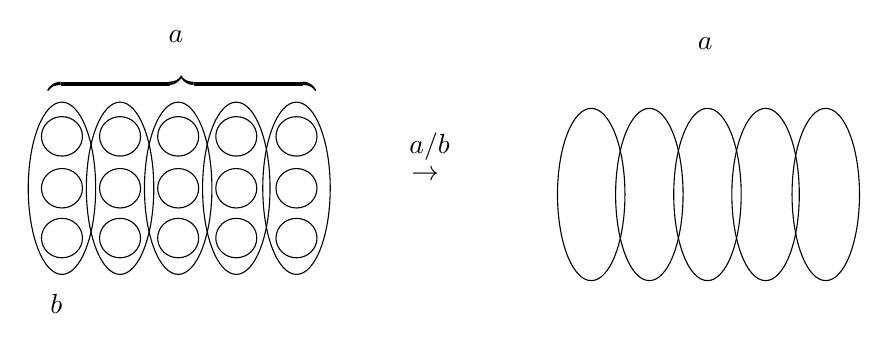
\begin{tikzpicture}[x=0.75pt,y=0.75pt,yscale=-1,xscale=1]
%uncomment if require: \path (0,300); %set diagram left start at 0, and has height of 300

%Shape: Ellipse [id:dp7671574737022798] 
\draw   (396.63,166.5) .. controls (396.63,143.58) and (403.9,125) .. (412.88,125) .. controls (421.85,125) and (429.13,143.58) .. (429.13,166.5) .. controls (429.13,189.42) and (421.85,208) .. (412.88,208) .. controls (403.9,208) and (396.63,189.42) .. (396.63,166.5) -- cycle ;
%Shape: Ellipse [id:dp31275198164884266] 
\draw   (424.63,166.5) .. controls (424.63,143.58) and (431.9,125) .. (440.88,125) .. controls (449.85,125) and (457.13,143.58) .. (457.13,166.5) .. controls (457.13,189.42) and (449.85,208) .. (440.88,208) .. controls (431.9,208) and (424.63,189.42) .. (424.63,166.5) -- cycle ;
%Shape: Ellipse [id:dp46551803266199265] 
\draw   (452.63,166.5) .. controls (452.63,143.58) and (459.9,125) .. (468.88,125) .. controls (477.85,125) and (485.13,143.58) .. (485.13,166.5) .. controls (485.13,189.42) and (477.85,208) .. (468.88,208) .. controls (459.9,208) and (452.63,189.42) .. (452.63,166.5) -- cycle ;
%Shape: Ellipse [id:dp18999430427046538] 
\draw   (480.63,166.5) .. controls (480.63,143.58) and (487.9,125) .. (496.88,125) .. controls (505.85,125) and (513.13,143.58) .. (513.13,166.5) .. controls (513.13,189.42) and (505.85,208) .. (496.88,208) .. controls (487.9,208) and (480.63,189.42) .. (480.63,166.5) -- cycle ;
%Shape: Ellipse [id:dp7957215995179295] 
\draw   (509.63,166.5) .. controls (509.63,143.58) and (516.9,125) .. (525.88,125) .. controls (534.85,125) and (542.13,143.58) .. (542.13,166.5) .. controls (542.13,189.42) and (534.85,208) .. (525.88,208) .. controls (516.9,208) and (509.63,189.42) .. (509.63,166.5) -- cycle ;
%Shape: Ellipse [id:dp11314566128963044] 
\draw   (148,138.5) .. controls (148,133.25) and (152.42,129) .. (157.88,129) .. controls (163.33,129) and (167.75,133.25) .. (167.75,138.5) .. controls (167.75,143.75) and (163.33,148) .. (157.88,148) .. controls (152.42,148) and (148,143.75) .. (148,138.5) -- cycle ;
%Shape: Ellipse [id:dp20342543709143968] 
\draw   (176,138.5) .. controls (176,133.25) and (180.42,129) .. (185.88,129) .. controls (191.33,129) and (195.75,133.25) .. (195.75,138.5) .. controls (195.75,143.75) and (191.33,148) .. (185.88,148) .. controls (180.42,148) and (176,143.75) .. (176,138.5) -- cycle ;
%Shape: Ellipse [id:dp06114935748386208] 
\draw   (204,138.5) .. controls (204,133.25) and (208.42,129) .. (213.88,129) .. controls (219.33,129) and (223.75,133.25) .. (223.75,138.5) .. controls (223.75,143.75) and (219.33,148) .. (213.88,148) .. controls (208.42,148) and (204,143.75) .. (204,138.5) -- cycle ;
%Shape: Ellipse [id:dp6126055210358686] 
\draw   (232,138.5) .. controls (232,133.25) and (236.42,129) .. (241.88,129) .. controls (247.33,129) and (251.75,133.25) .. (251.75,138.5) .. controls (251.75,143.75) and (247.33,148) .. (241.88,148) .. controls (236.42,148) and (232,143.75) .. (232,138.5) -- cycle ;
%Shape: Ellipse [id:dp5477621350161328] 
\draw   (261,138.5) .. controls (261,133.25) and (265.42,129) .. (270.88,129) .. controls (276.33,129) and (280.75,133.25) .. (280.75,138.5) .. controls (280.75,143.75) and (276.33,148) .. (270.88,148) .. controls (265.42,148) and (261,143.75) .. (261,138.5) -- cycle ;
%Shape: Ellipse [id:dp3795127345430579] 
\draw   (148,163.5) .. controls (148,158.25) and (152.42,154) .. (157.88,154) .. controls (163.33,154) and (167.75,158.25) .. (167.75,163.5) .. controls (167.75,168.75) and (163.33,173) .. (157.88,173) .. controls (152.42,173) and (148,168.75) .. (148,163.5) -- cycle ;
%Shape: Ellipse [id:dp7947843476789982] 
\draw   (176,163.5) .. controls (176,158.25) and (180.42,154) .. (185.88,154) .. controls (191.33,154) and (195.75,158.25) .. (195.75,163.5) .. controls (195.75,168.75) and (191.33,173) .. (185.88,173) .. controls (180.42,173) and (176,168.75) .. (176,163.5) -- cycle ;
%Shape: Ellipse [id:dp2274431585986295] 
\draw   (204,163.5) .. controls (204,158.25) and (208.42,154) .. (213.88,154) .. controls (219.33,154) and (223.75,158.25) .. (223.75,163.5) .. controls (223.75,168.75) and (219.33,173) .. (213.88,173) .. controls (208.42,173) and (204,168.75) .. (204,163.5) -- cycle ;
%Shape: Ellipse [id:dp03681681086349042] 
\draw   (232,163.5) .. controls (232,158.25) and (236.42,154) .. (241.88,154) .. controls (247.33,154) and (251.75,158.25) .. (251.75,163.5) .. controls (251.75,168.75) and (247.33,173) .. (241.88,173) .. controls (236.42,173) and (232,168.75) .. (232,163.5) -- cycle ;
%Shape: Ellipse [id:dp31634570761817327] 
\draw   (261,163.5) .. controls (261,158.25) and (265.42,154) .. (270.88,154) .. controls (276.33,154) and (280.75,158.25) .. (280.75,163.5) .. controls (280.75,168.75) and (276.33,173) .. (270.88,173) .. controls (265.42,173) and (261,168.75) .. (261,163.5) -- cycle ;
%Shape: Ellipse [id:dp9901002407853906] 
\draw   (148,187.5) .. controls (148,182.25) and (152.42,178) .. (157.88,178) .. controls (163.33,178) and (167.75,182.25) .. (167.75,187.5) .. controls (167.75,192.75) and (163.33,197) .. (157.88,197) .. controls (152.42,197) and (148,192.75) .. (148,187.5) -- cycle ;
%Shape: Ellipse [id:dp5537390438494408] 
\draw   (176,187.5) .. controls (176,182.25) and (180.42,178) .. (185.88,178) .. controls (191.33,178) and (195.75,182.25) .. (195.75,187.5) .. controls (195.75,192.75) and (191.33,197) .. (185.88,197) .. controls (180.42,197) and (176,192.75) .. (176,187.5) -- cycle ;
%Shape: Ellipse [id:dp6171434670538515] 
\draw   (204,187.5) .. controls (204,182.25) and (208.42,178) .. (213.88,178) .. controls (219.33,178) and (223.75,182.25) .. (223.75,187.5) .. controls (223.75,192.75) and (219.33,197) .. (213.88,197) .. controls (208.42,197) and (204,192.75) .. (204,187.5) -- cycle ;
%Shape: Ellipse [id:dp2625784329084404] 
\draw   (232,187.5) .. controls (232,182.25) and (236.42,178) .. (241.88,178) .. controls (247.33,178) and (251.75,182.25) .. (251.75,187.5) .. controls (251.75,192.75) and (247.33,197) .. (241.88,197) .. controls (236.42,197) and (232,192.75) .. (232,187.5) -- cycle ;
%Shape: Ellipse [id:dp2680369611777734] 
\draw   (261,187.5) .. controls (261,182.25) and (265.42,178) .. (270.88,178) .. controls (276.33,178) and (280.75,182.25) .. (280.75,187.5) .. controls (280.75,192.75) and (276.33,197) .. (270.88,197) .. controls (265.42,197) and (261,192.75) .. (261,187.5) -- cycle ;
%Shape: Ellipse [id:dp5261526305335597] 
\draw   (141.63,163.5) .. controls (141.63,140.58) and (148.9,122) .. (157.88,122) .. controls (166.85,122) and (174.13,140.58) .. (174.13,163.5) .. controls (174.13,186.42) and (166.85,205) .. (157.88,205) .. controls (148.9,205) and (141.63,186.42) .. (141.63,163.5) -- cycle ;
%Shape: Ellipse [id:dp2541396817752227] 
\draw   (169.63,163.5) .. controls (169.63,140.58) and (176.9,122) .. (185.88,122) .. controls (194.85,122) and (202.13,140.58) .. (202.13,163.5) .. controls (202.13,186.42) and (194.85,205) .. (185.88,205) .. controls (176.9,205) and (169.63,186.42) .. (169.63,163.5) -- cycle ;
%Shape: Ellipse [id:dp04577032474970055] 
\draw   (197.63,163.5) .. controls (197.63,140.58) and (204.9,122) .. (213.88,122) .. controls (222.85,122) and (230.13,140.58) .. (230.13,163.5) .. controls (230.13,186.42) and (222.85,205) .. (213.88,205) .. controls (204.9,205) and (197.63,186.42) .. (197.63,163.5) -- cycle ;
%Shape: Ellipse [id:dp596542665939238] 
\draw   (225.63,163.5) .. controls (225.63,140.58) and (232.9,122) .. (241.88,122) .. controls (250.85,122) and (258.13,140.58) .. (258.13,163.5) .. controls (258.13,186.42) and (250.85,205) .. (241.88,205) .. controls (232.9,205) and (225.63,186.42) .. (225.63,163.5) -- cycle ;
%Shape: Ellipse [id:dp36960768390890764] 
\draw   (254.63,163.5) .. controls (254.63,140.58) and (261.9,122) .. (270.88,122) .. controls (279.85,122) and (287.13,140.58) .. (287.13,163.5) .. controls (287.13,186.42) and (279.85,205) .. (270.88,205) .. controls (261.9,205) and (254.63,186.42) .. (254.63,163.5) -- cycle ;

% Text Node
\draw (463,89.4) node [anchor=north west][inner sep=0.75pt]    {$a$};
% Text Node
\draw (208,86.4) node [anchor=north west][inner sep=0.75pt]    {$a$};
% Text Node
\draw (150,108.4) node [anchor=north west][inner sep=0.75pt]    {$\overbrace{\ \ \ \ \ \ \ \ \ \ \ \ \ \ \ \ \ \ \ \ \ \ \ \ \ \ \ \ \ }$};
% Text Node
\draw (151,213.4) node [anchor=north west][inner sep=0.75pt]    {$b$};
% Text Node
\draw (325,153.4) node [anchor=north west][inner sep=0.75pt]    {$\rightarrow $};
% Text Node
\draw (324,135.4) node [anchor=north west][inner sep=0.75pt]    {$a/b$};


\end{tikzpicture}

This is like quotienting out \( b \) and considering it as the new unit.

Alternatively, you can think of it as making \( a \) groups of \( 1/b \).


\subsubsection{Ratios}

Another way to think about division is as a ratio.
Given \( a/b \), if \( b \) were a measuring stick, how big would we measure \( a \) as?
Sometimes, we don't know this answer but we can still compare ratios.
If we have \( a/b \) and \( c/d \), we can put the measuring sticks together into one big one.
In order to match them up, we find the least common multiple \( bd \).
Then in terms of the new ruler, we have \( ad/bd \) and \( cb/db \).


\subsection{Exponentiation}

Suppose a culture of bacteria replicates at a rate such that it doubles every hour.
We start with one bacterium at time \( t = 0 \).
Then every hour after that, the number of bacteria is twice the number an hour previously.
The number at time \( t \) can be found by repeatedly multiplying:
\( 2^t = \underbrace{2 \cdot 2 \cdot \ldots \cdot 2}_t \).

\noindent
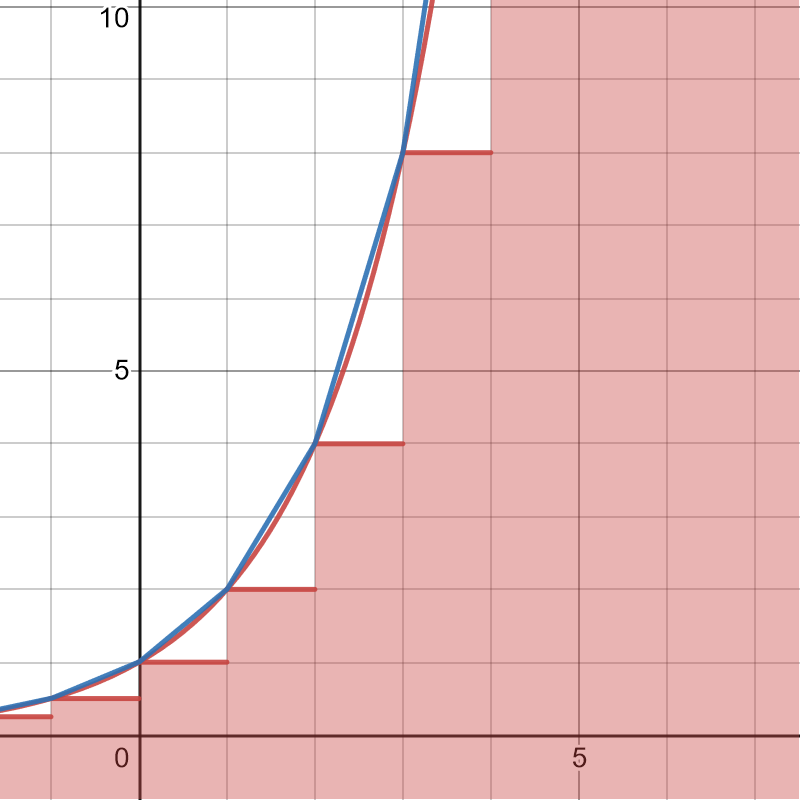
\includegraphics[width=\textwidth]{desmos-graph.png}

The previous gives us a model for discrete growth,
but now what if we wanted to talk about continuous growth?
We would still like to keep the rate so that it doubled every time step.

If we only examine the growth during 1 time step,
we can break down the growth into partial amount like so.

\tikzset{every picture/.style={line width=0.75pt}} %set default line width to 0.75pt        

\noindent
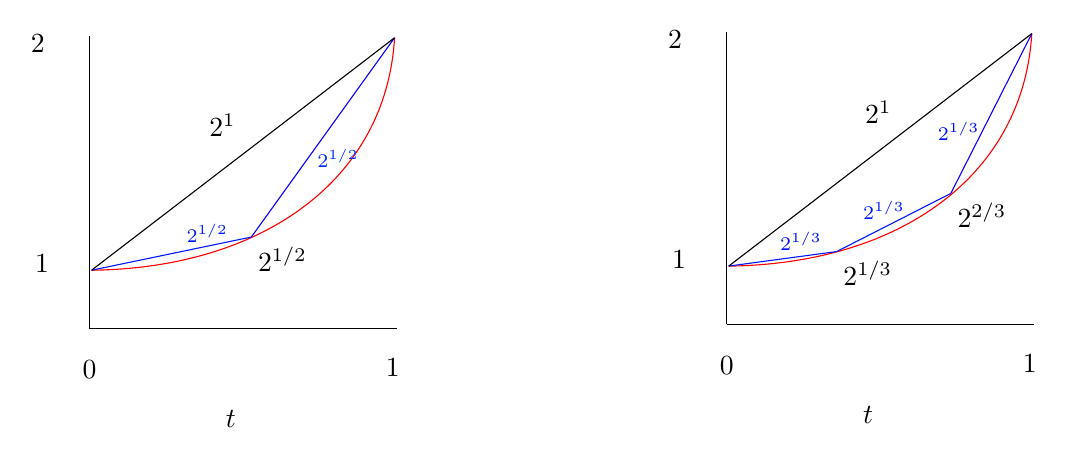
\begin{tikzpicture}[x=0.75pt,y=0.75pt,yscale=-1,xscale=1]
%uncomment if require: \path (0,300); %set diagram left start at 0, and has height of 300

%Curve Lines [id:da026757245325067736] 
\draw [color={rgb, 255:red, 255; green, 0; blue, 0 }  ,draw opacity=1 ]   (113.5,191) .. controls (196.5,190) and (255.5,147) .. (259.5,79) ;
%Straight Lines [id:da8207839175944438] 
\draw    (112.5,219) -- (260.5,219) ;
%Straight Lines [id:da8786334522061489] 
\draw    (112.5,78) -- (112.5,219) ;
%Straight Lines [id:da5179270946161231] 
\draw [color={rgb, 255:red, 0; green, 24; blue, 253 }  ,draw opacity=1 ]   (113.5,191) -- (190.5,175) ;
%Straight Lines [id:da005954831626670876] 
\draw [color={rgb, 255:red, 12; green, 0; blue, 255 }  ,draw opacity=1 ]   (259.5,79) -- (190.5,175) ;
%Curve Lines [id:da12339674961297564] 
\draw [color={rgb, 255:red, 255; green, 0; blue, 0 }  ,draw opacity=1 ]   (420.5,189) .. controls (503.5,188) and (562.5,145) .. (566.5,77) ;
%Straight Lines [id:da8738046986203857] 
\draw    (419.5,217) -- (567.5,217) ;
%Straight Lines [id:da7821696604444603] 
\draw    (419.5,76) -- (419.5,217) ;
%Straight Lines [id:da7563442671168474] 
\draw [color={rgb, 255:red, 0; green, 24; blue, 253 }  ,draw opacity=1 ]   (420.5,189) -- (472.5,182) ;
%Straight Lines [id:da81713435283311] 
\draw [color={rgb, 255:red, 12; green, 0; blue, 255 }  ,draw opacity=1 ]   (566.5,77) -- (527.5,154) ;
%Straight Lines [id:da8759585096736938] 
\draw    (113.5,191) -- (259.5,79) ;
%Straight Lines [id:da784575567252201] 
\draw    (420.5,189) -- (566.5,77) ;
%Straight Lines [id:da05035012565036756] 
\draw [color={rgb, 255:red, 0; green, 24; blue, 253 }  ,draw opacity=1 ]   (472.5,182) -- (527.5,154) ;

% Text Node
\draw (108,233.4) node [anchor=north west][inner sep=0.75pt]    {$0$};
% Text Node
\draw (254,232.4) node [anchor=north west][inner sep=0.75pt]    {$1$};
% Text Node
\draw (177,257.4) node [anchor=north west][inner sep=0.75pt]    {$t$};
% Text Node
\draw (85,182.4) node [anchor=north west][inner sep=0.75pt]    {$1$};
% Text Node
\draw (83,76.4) node [anchor=north west][inner sep=0.75pt]    {$2$};
% Text Node
\draw (192.5,178.4) node [anchor=north west][inner sep=0.75pt]    {$2^{1/2}$};
% Text Node
\draw (415,231.4) node [anchor=north west][inner sep=0.75pt]    {$0$};
% Text Node
\draw (561,230.4) node [anchor=north west][inner sep=0.75pt]    {$1$};
% Text Node
\draw (484,255.4) node [anchor=north west][inner sep=0.75pt]    {$t$};
% Text Node
\draw (392,180.4) node [anchor=north west][inner sep=0.75pt]    {$1$};
% Text Node
\draw (390,74.4) node [anchor=north west][inner sep=0.75pt]    {$2$};
% Text Node
\draw (474.5,185.4) node [anchor=north west][inner sep=0.75pt]    {$2^{1/3}$};
% Text Node
\draw (169,114.4) node [anchor=north west][inner sep=0.75pt]    {$2^{1}$};
% Text Node
\draw (485,108.4) node [anchor=north west][inner sep=0.75pt]    {$2^{1}$};
% Text Node
\draw (529.5,157.4) node [anchor=north west][inner sep=0.75pt]    {$2^{2/3}$};
% Text Node
\draw (158,167.4) node [anchor=north west][inner sep=0.75pt]  [font=\scriptsize,color={rgb, 255:red, 0; green, 24; blue, 255 }  ,opacity=1 ]  {$2^{1/2}$};
% Text Node
\draw (221,131.4) node [anchor=north west][inner sep=0.75pt]  [font=\scriptsize,color={rgb, 255:red, 0; green, 42; blue, 255 }  ,opacity=1 ]  {$2^{1/2}$};
% Text Node
\draw (444,171.4) node [anchor=north west][inner sep=0.75pt]  [font=\scriptsize,color={rgb, 255:red, 0; green, 15; blue, 255 }  ,opacity=1 ]  {$2^{1/3}$};
% Text Node
\draw (484,156.4) node [anchor=north west][inner sep=0.75pt]  [font=\scriptsize,color={rgb, 255:red, 0; green, 24; blue, 255 }  ,opacity=1 ]  {$2^{1/3}$};
% Text Node
\draw (520,118.4) node [anchor=north west][inner sep=0.75pt]  [font=\scriptsize,color={rgb, 255:red, 0; green, 15; blue, 255 }  ,opacity=1 ]  {$2^{1/3}$};


\end{tikzpicture}

The blue lines represent multiplying by partial proportions.
We define partial growth so that the proportions taken together is the same as the original
\( 2^{1/2} \cdot 2^{1/2} = 2^1 \).

We can do this in general for any real number \( t \) and \( b \).

\tikzset{every picture/.style={line width=0.75pt}} %set default line width to 0.75pt        

\noindent
\begin{center}
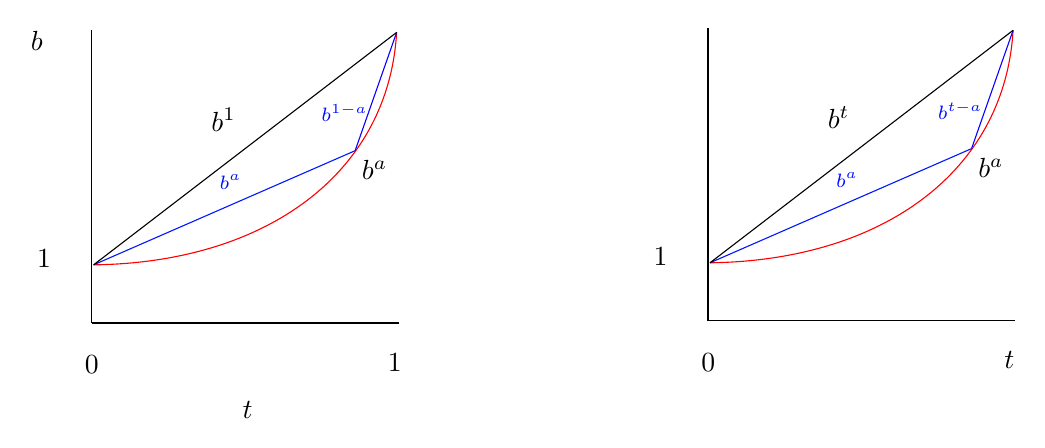
\begin{tikzpicture}[x=0.75pt,y=0.75pt,yscale=-1,xscale=1]
%uncomment if require: \path (0,300); %set diagram left start at 0, and has height of 300

%Curve Lines [id:da004250453094733597] 
\draw [color={rgb, 255:red, 255; green, 0; blue, 0 }  ,draw opacity=1 ]   (399.5,174) .. controls (482.5,173) and (541.5,130) .. (545.5,62) ;
%Straight Lines [id:da11185903183918833] 
\draw    (398.5,202) -- (546.5,202) ;
%Straight Lines [id:da2683371977344995] 
\draw    (398.5,61) -- (398.5,202) ;
%Straight Lines [id:da4582386497031067] 
\draw [color={rgb, 255:red, 0; green, 24; blue, 253 }  ,draw opacity=1 ]   (399.5,174) -- (525.5,119) ;
%Straight Lines [id:da2975129059808127] 
\draw [color={rgb, 255:red, 12; green, 0; blue, 255 }  ,draw opacity=1 ]   (545.5,62) -- (525.5,119) ;
%Straight Lines [id:da8666491434636445] 
\draw    (399.5,174) -- (545.5,62) ;
%Curve Lines [id:da8968805547814415] 
\draw [color={rgb, 255:red, 255; green, 0; blue, 0 }  ,draw opacity=1 ]   (102.5,175) .. controls (185.5,174) and (244.5,131) .. (248.5,63) ;
%Straight Lines [id:da4205745305765404] 
\draw    (101.5,203) -- (249.5,203) ;
%Straight Lines [id:da17942895279134785] 
\draw    (101.5,62) -- (101.5,203) ;
%Straight Lines [id:da8844445030454833] 
\draw [color={rgb, 255:red, 0; green, 24; blue, 253 }  ,draw opacity=1 ]   (102.5,175) -- (228.5,120) ;
%Straight Lines [id:da840463859307833] 
\draw [color={rgb, 255:red, 12; green, 0; blue, 255 }  ,draw opacity=1 ]   (248.5,63) -- (228.5,120) ;
%Straight Lines [id:da14755909330885852] 
\draw    (102.5,175) -- (248.5,63) ;

% Text Node
\draw (394,216.4) node [anchor=north west][inner sep=0.75pt]    {$0$};
% Text Node
\draw (540,215.4) node [anchor=north west][inner sep=0.75pt]    {$t$};
% Text Node
\draw (371,165.4) node [anchor=north west][inner sep=0.75pt]    {$1$};
% Text Node
\draw (527.5,122.4) node [anchor=north west][inner sep=0.75pt]    {$b^{a}$};
% Text Node
\draw (455,97.4) node [anchor=north west][inner sep=0.75pt]    {$b^{t}$};
% Text Node
\draw (459,129.4) node [anchor=north west][inner sep=0.75pt]  [font=\scriptsize,color={rgb, 255:red, 0; green, 15; blue, 255 }  ,opacity=1 ]  {$b^{a}$};
% Text Node
\draw (508,95.4) node [anchor=north west][inner sep=0.75pt]  [font=\scriptsize,color={rgb, 255:red, 0; green, 15; blue, 255 }  ,opacity=1 ]  {$b^{t-a}$};
% Text Node
\draw (97,217.4) node [anchor=north west][inner sep=0.75pt]    {$0$};
% Text Node
\draw (243,216.4) node [anchor=north west][inner sep=0.75pt]    {$1$};
% Text Node
\draw (74,166.4) node [anchor=north west][inner sep=0.75pt]    {$1$};
% Text Node
\draw (230.5,123.4) node [anchor=north west][inner sep=0.75pt]    {$b^{a}$};
% Text Node
\draw (158,98.4) node [anchor=north west][inner sep=0.75pt]    {$b^{1}$};
% Text Node
\draw (162,130.4) node [anchor=north west][inner sep=0.75pt]  [font=\scriptsize,color={rgb, 255:red, 0; green, 15; blue, 255 }  ,opacity=1 ]  {$b^{a}$};
% Text Node
\draw (211,96.4) node [anchor=north west][inner sep=0.75pt]  [font=\scriptsize,color={rgb, 255:red, 0; green, 15; blue, 255 }  ,opacity=1 ]  {$b^{1-a}$};
% Text Node
\draw (71,61.4) node [anchor=north west][inner sep=0.75pt]    {$b$};
% Text Node
\draw (173,239.4) node [anchor=north west][inner sep=0.75pt]    {$t$};


\end{tikzpicture}
\end{center}

This also gives intuition for negative exponents
as 'reversing time' or dividing by a proportion instead of multiplying.

Exponentiation is a natural extension of repeated multiplication
to continuous multiplicative growth.
It is convenient to define the continuous growth so that it is 'benchmarked'
at the given proportion every time step.
That is, for every \( t \), we multiply by \( b \),
and partial growth is defined so that the total proportion is just the product of the partials.

\newpage
\subsubsection{Different bases}

To think about different bases, think of scaling the \( x \)-axis so that
the amount at time 1 is always the base.

\tikzset{every picture/.style={line width=0.75pt}} %set default line width to 0.75pt        

\noindent
\begin{tikzpicture}[x=0.75pt,y=0.75pt,yscale=-0.8,xscale=0.8]
%uncomment if require: \path (0,300); %set diagram left start at 0, and has height of 300

%Curve Lines [id:da7831591201331012] 
\draw [color={rgb, 255:red, 255; green, 0; blue, 0 }  ,draw opacity=1 ]   (83.15,192.12) .. controls (207.44,190.62) and (295.8,126.23) .. (301.79,24.4) ;
%Straight Lines [id:da6727010717613063] 
\draw    (81.65,234.05) -- (303.28,234.05) ;
%Straight Lines [id:da18291760297885706] 
\draw    (81.65,22.9) -- (81.65,234.05) ;
%Shape: Circle [id:dp9221594920848606] 
\draw   (169,179) .. controls (169,177.9) and (169.9,177) .. (171,177) .. controls (172.1,177) and (173,177.9) .. (173,179) .. controls (173,180.1) and (172.1,181) .. (171,181) .. controls (169.9,181) and (169,180.1) .. (169,179) -- cycle ;
%Curve Lines [id:da05008353068018789] 
\draw [color={rgb, 255:red, 255; green, 0; blue, 0 }  ,draw opacity=1 ]   (400.15,195.12) .. controls (524.44,193.62) and (612.8,129.23) .. (618.79,27.4) ;
%Straight Lines [id:da2168148480276918] 
\draw    (398.65,237.05) -- (620.28,237.05) ;
%Straight Lines [id:da5164683642298775] 
\draw    (398.65,25.9) -- (398.65,237.05) ;
%Shape: Circle [id:dp4971686037061359] 
\draw   (547,153) .. controls (547,151.9) and (547.9,151) .. (549,151) .. controls (550.1,151) and (551,151.9) .. (551,153) .. controls (551,154.1) and (550.1,155) .. (549,155) .. controls (547.9,155) and (547,154.1) .. (547,153) -- cycle ;

% Text Node
\draw (77.9,249.4) node [anchor=north west][inner sep=0.75pt]    {$0$};
% Text Node
\draw (51,183.4) node [anchor=north west][inner sep=0.75pt]    {$1$};
% Text Node
\draw (173,180.4) node [anchor=north west][inner sep=0.75pt]    {$b$};
% Text Node
\draw (169,250.4) node [anchor=north west][inner sep=0.75pt]    {$1$};
% Text Node
\draw (394.9,252.4) node [anchor=north west][inner sep=0.75pt]    {$0$};
% Text Node
\draw (368,186.4) node [anchor=north west][inner sep=0.75pt]    {$1$};
% Text Node
\draw (553,156.4) node [anchor=north west][inner sep=0.75pt]    {$c$};
% Text Node
\draw (551,248.4) node [anchor=north west][inner sep=0.75pt]    {$1$};
% Text Node
\draw (156,42.4) node [anchor=north west][inner sep=0.75pt]    {$b^{t}$};
% Text Node
\draw (490,33.4) node [anchor=north west][inner sep=0.75pt]    {$c^{t}$};


\end{tikzpicture}

\subsubsection{Memorylessness}

Because we are working with proportions rather than any specific amounts,
exponential functions are 'memoryless' (you can 'forget' the zero point).
That is, the amount of growth in any given time interval \( t \)
is always the same proportion regardless of when we take that interval.

\noindent
\begin{tikzpicture}[x=0.75pt,y=0.75pt,yscale=-0.8,xscale=0.8]
%uncomment if require: \path (0,300); %set diagram left start at 0, and has height of 300

%Curve Lines [id:da16505242416400712] 
\draw [color={rgb, 255:red, 255; green, 0; blue, 0 }  ,draw opacity=1 ]   (103.15,205.12) .. controls (227.44,203.62) and (315.8,139.23) .. (321.79,37.4) ;
%Straight Lines [id:da7267676985584549] 
\draw    (101.65,247.05) -- (323.28,247.05) ;
%Straight Lines [id:da4645289606705647] 
\draw    (101.65,35.9) -- (101.65,247.05) ;
%Shape: Circle [id:dp39770385046406675] 
\draw   (189,192) .. controls (189,190.9) and (189.9,190) .. (191,190) .. controls (192.1,190) and (193,190.9) .. (193,192) .. controls (193,193.1) and (192.1,194) .. (191,194) .. controls (189.9,194) and (189,193.1) .. (189,192) -- cycle ;
%Straight Lines [id:da1118098783506678] 
\draw [color={rgb, 255:red, 0; green, 50; blue, 255 }  ,draw opacity=1 ]   (103.15,205.12) -- (256.5,160) ;
%Shape: Brace [id:dp33401170253306967] 
\draw   (102,208) .. controls (102,212.67) and (104.33,215) .. (109,215) -- (172.25,215) .. controls (178.92,215) and (182.25,217.33) .. (182.25,222) .. controls (182.25,217.33) and (185.58,215) .. (192.25,215)(189.25,215) -- (255.5,215) .. controls (260.17,215) and (262.5,212.67) .. (262.5,208) ;
%Curve Lines [id:da702343555310466] 
\draw [color={rgb, 255:red, 255; green, 0; blue, 0 }  ,draw opacity=1 ]   (408.15,203.12) .. controls (532.44,201.62) and (620.8,137.23) .. (626.79,35.4) ;
%Straight Lines [id:da5457712288003155] 
\draw    (406.65,245.05) -- (628.28,245.05) ;
%Straight Lines [id:da6145389316373155] 
\draw    (406.65,33.9) -- (406.65,245.05) ;
%Shape: Circle [id:dp8592795818420744] 
\draw   (494,190) .. controls (494,188.9) and (494.9,188) .. (496,188) .. controls (497.1,188) and (498,188.9) .. (498,190) .. controls (498,191.1) and (497.1,192) .. (496,192) .. controls (494.9,192) and (494,191.1) .. (494,190) -- cycle ;
%Straight Lines [id:da9754483079369636] 
\draw [color={rgb, 255:red, 0; green, 42; blue, 255 }  ,draw opacity=1 ]   (461.5,198) -- (619.5,76) ;
%Shape: Brace [id:dp4810786659509392] 
\draw   (463,205) .. controls (463,209.67) and (465.33,212) .. (470,212) -- (533.25,212) .. controls (539.92,212) and (543.25,214.33) .. (543.25,219) .. controls (543.25,214.33) and (546.58,212) .. (553.25,212)(550.25,212) -- (616.5,212) .. controls (621.17,212) and (623.5,209.67) .. (623.5,205) ;

% Text Node
\draw (97.9,262.4) node [anchor=north west][inner sep=0.75pt]    {$0$};
% Text Node
\draw (71,196.4) node [anchor=north west][inner sep=0.75pt]    {$1$};
% Text Node
\draw (193,193.4) node [anchor=north west][inner sep=0.75pt]    {$b$};
% Text Node
\draw (189,263.4) node [anchor=north west][inner sep=0.75pt]    {$1$};
% Text Node
\draw (178,155.4) node [anchor=north west][inner sep=0.75pt]  [color={rgb, 255:red, 0; green, 33; blue, 255 }  ,opacity=1 ]  {$b^{c}$};
% Text Node
\draw (177,222.4) node [anchor=north west][inner sep=0.75pt]    {$c$};
% Text Node
\draw (402.9,260.4) node [anchor=north west][inner sep=0.75pt]    {$0$};
% Text Node
\draw (376,194.4) node [anchor=north west][inner sep=0.75pt]    {$1$};
% Text Node
\draw (498,191.4) node [anchor=north west][inner sep=0.75pt]    {$b$};
% Text Node
\draw (494,261.4) node [anchor=north west][inner sep=0.75pt]    {$1$};
% Text Node
\draw (518,120.4) node [anchor=north west][inner sep=0.75pt]  [color={rgb, 255:red, 0; green, 24; blue, 255 }  ,opacity=1 ]  {$b^{c}$};
% Text Node
\draw (538,219.4) node [anchor=north west][inner sep=0.75pt]    {$c$};
% Text Node
\draw (258.5,163.4) node [anchor=north west][inner sep=0.75pt]    {$b^{c}$};
% Text Node
\draw (450,176.4) node [anchor=north west][inner sep=0.75pt]    {$a$};
% Text Node
\draw (621.5,79.4) node [anchor=north west][inner sep=0.75pt]    {$ab^{c}$};

\end{tikzpicture}

This is convenient since it allows us to only about proportions
without thinking about amounts.
That is, we can think of \( b^t \) as the proportion of growth that happens in a \( t \)
time interval.

\newpage
\subsubsection{Rules}

The rule \( a^{b+c} = a^b a^c \) says that adding \( c \) to growth time
is the same as multiplying by aother proportion of \( a^c \).

\begin{center}
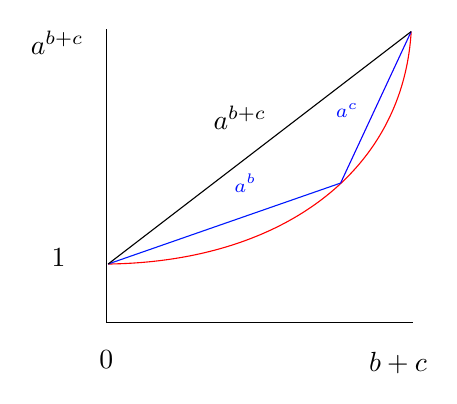
\begin{tikzpicture}[x=0.75pt,y=0.75pt,yscale=-1,xscale=1]
%uncomment if require: \path (0,300); %set diagram left start at 0, and has height of 300

%Curve Lines [id:da7648292128629934] 
\draw [color={rgb, 255:red, 255; green, 0; blue, 0 }  ,draw opacity=1 ]   (114.5,175) .. controls (197.5,174) and (256.5,131) .. (260.5,63) ;
%Straight Lines [id:da7623123576251518] 
\draw    (113.5,203) -- (261.5,203) ;
%Straight Lines [id:da45171993306474634] 
\draw    (113.5,62) -- (113.5,203) ;
%Straight Lines [id:da11496418575904588] 
\draw [color={rgb, 255:red, 0; green, 24; blue, 253 }  ,draw opacity=1 ]   (114.5,175) -- (226.5,136) ;
%Straight Lines [id:da9303796173825488] 
\draw [color={rgb, 255:red, 12; green, 0; blue, 255 }  ,draw opacity=1 ]   (260.5,63) -- (226.5,136) ;
%Straight Lines [id:da30716669420649056] 
\draw    (114.5,175) -- (260.5,63) ;

% Text Node
\draw (109,215.4) node [anchor=north west][inner sep=0.75pt]    {$0$};
% Text Node
\draw (239,216.4) node [anchor=north west][inner sep=0.75pt]    {$b+c$};
% Text Node
\draw (86,166.4) node [anchor=north west][inner sep=0.75pt]    {$1$};
% Text Node
\draw (164,97.4) node [anchor=north west][inner sep=0.75pt]    {$a^{b+c}$};
% Text Node
\draw (174,130.4) node [anchor=north west][inner sep=0.75pt]  [font=\scriptsize,color={rgb, 255:red, 0; green, 15; blue, 255 }  ,opacity=1 ]  {$a^{b}$};
% Text Node
\draw (223,96.4) node [anchor=north west][inner sep=0.75pt]  [font=\scriptsize,color={rgb, 255:red, 0; green, 15; blue, 255 }  ,opacity=1 ]  {$a^{c}$};
% Text Node
\draw (76,61.4) node [anchor=north west][inner sep=0.75pt]    {$a^{b+c}$};


\end{tikzpicture}
\end{center}

The rule \( (a^{b})^{c} = a^{bc} \) says that if we take \( p^c \)
but we express our base proportion \( p \)
as a exponentiation of a different proportion \( p = a^b \),
then the result can be expressed as \( a^{bc} \).

\noindent
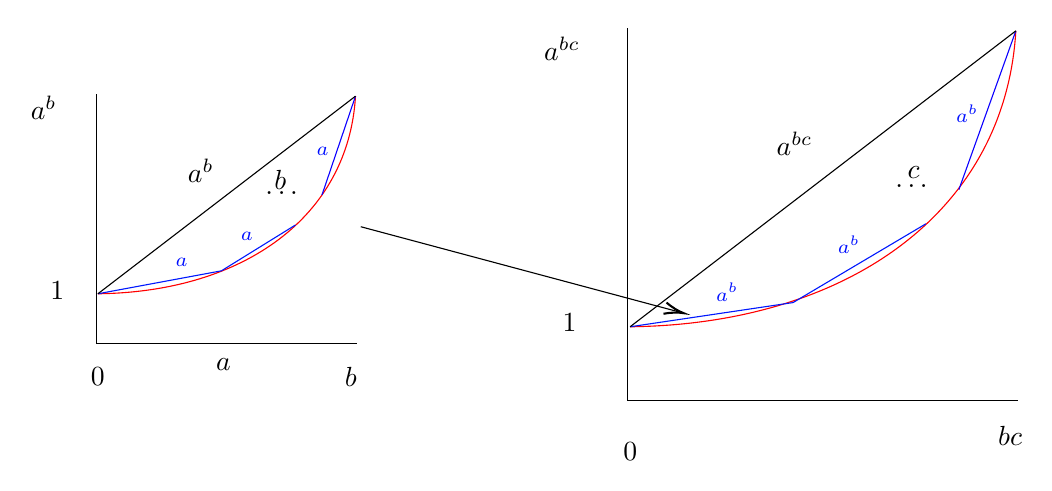
\begin{tikzpicture}[x=0.75pt,y=0.75pt,yscale=-0.85,xscale=0.85]
%uncomment if require: \path (0,300); %set diagram left start at 0, and has height of 300

%Curve Lines [id:da09645713901037456] 
\draw [color={rgb, 255:red, 255; green, 0; blue, 0 }  ,draw opacity=1 ]   (374.15,191.71) .. controls (498.44,190.21) and (586.8,125.82) .. (592.79,23.99) ;
%Straight Lines [id:da6655564601424763] 
\draw    (372.65,233.64) -- (594.28,233.64) ;
%Straight Lines [id:da20638279854797614] 
\draw    (372.65,22.49) -- (372.65,233.64) ;
%Straight Lines [id:da7813965411778568] 
\draw [color={rgb, 255:red, 0; green, 24; blue, 253 }  ,draw opacity=1 ]   (374.15,191.71) -- (466.5,178) ;
%Straight Lines [id:da4249104214147267] 
\draw [color={rgb, 255:red, 12; green, 0; blue, 255 }  ,draw opacity=1 ]   (592.79,23.99) -- (560.5,114) ;
%Straight Lines [id:da38364756594044924] 
\draw    (374.15,191.71) -- (592.79,23.99) ;
%Straight Lines [id:da5538051163006323] 
\draw [color={rgb, 255:red, 0; green, 24; blue, 253 }  ,draw opacity=1 ]   (466.5,178) -- (541.87,133.31) ;
%Curve Lines [id:da5159608570475862] 
\draw [color={rgb, 255:red, 255; green, 0; blue, 0 }  ,draw opacity=1 ]   (72.5,173) .. controls (155.5,172) and (214.5,129) .. (218.5,61) ;
%Straight Lines [id:da6841121300606191] 
\draw    (71.5,201) -- (219.5,201) ;
%Straight Lines [id:da7989643621039341] 
\draw    (71.5,60) -- (71.5,201) ;
%Straight Lines [id:da5285327925330245] 
\draw [color={rgb, 255:red, 0; green, 24; blue, 253 }  ,draw opacity=1 ]   (72.5,173) -- (142.5,160) ;
%Straight Lines [id:da029865962698182424] 
\draw [color={rgb, 255:red, 12; green, 0; blue, 255 }  ,draw opacity=1 ]   (218.5,61) -- (199.5,117) ;
%Straight Lines [id:da9109218778484611] 
\draw    (72.5,173) -- (218.5,61) ;
%Straight Lines [id:da1833432740003489] 
\draw [color={rgb, 255:red, 0; green, 24; blue, 253 }  ,draw opacity=1 ]   (142.5,160) -- (184.5,134) ;
%Straight Lines [id:da572975186114413] 
\draw    (221.5,135) -- (402.57,183.48) ;
\draw [shift={(404.5,184)}, rotate = 194.99] [color={rgb, 255:red, 0; green, 0; blue, 0 }  ][line width=0.75]    (10.93,-3.29) .. controls (6.95,-1.4) and (3.31,-0.3) .. (0,0) .. controls (3.31,0.3) and (6.95,1.4) .. (10.93,3.29)   ;

% Text Node
\draw (368.9,255.99) node [anchor=north west][inner sep=0.75pt]    {$0$};
% Text Node
\draw (581.3,246.49) node [anchor=north west][inner sep=0.75pt]    {$bc$};
% Text Node
\draw (334.46,182.61) node [anchor=north west][inner sep=0.75pt]    {$1$};
% Text Node
\draw (455.74,79.78) node [anchor=north west][inner sep=0.75pt]    {$a^{bc}$};
% Text Node
\draw (421.49,165.46) node [anchor=north west][inner sep=0.75pt]  [font=\scriptsize,color={rgb, 255:red, 0; green, 15; blue, 255 }  ,opacity=1 ]  {$a^{b}$};
% Text Node
\draw (323.96,25.87) node [anchor=north west][inner sep=0.75pt]    {$a^{bc}$};
% Text Node
\draw (523,109.4) node [anchor=north west][inner sep=0.75pt]    {$\dotsc $};
% Text Node
\draw (530,99.4) node [anchor=north west][inner sep=0.75pt]    {$c$};
% Text Node
\draw (490.49,138.46) node [anchor=north west][inner sep=0.75pt]  [font=\scriptsize,color={rgb, 255:red, 0; green, 15; blue, 255 }  ,opacity=1 ]  {$a^{b}$};
% Text Node
\draw (557.49,64.46) node [anchor=north west][inner sep=0.75pt]  [font=\scriptsize,color={rgb, 255:red, 0; green, 15; blue, 255 }  ,opacity=1 ]  {$a^{b}$};
% Text Node
\draw (67,213.4) node [anchor=north west][inner sep=0.75pt]    {$0$};
% Text Node
\draw (211,213.4) node [anchor=north west][inner sep=0.75pt]    {$b$};
% Text Node
\draw (44,164.4) node [anchor=north west][inner sep=0.75pt]    {$1$};
% Text Node
\draw (122,95.4) node [anchor=north west][inner sep=0.75pt]    {$a^{b}$};
% Text Node
\draw (115,151.4) node [anchor=north west][inner sep=0.75pt]  [font=\scriptsize,color={rgb, 255:red, 0; green, 15; blue, 255 }  ,opacity=1 ]  {$a$};
% Text Node
\draw (195,88.4) node [anchor=north west][inner sep=0.75pt]  [font=\scriptsize,color={rgb, 255:red, 0; green, 15; blue, 255 }  ,opacity=1 ]  {$a$};
% Text Node
\draw (33,59.4) node [anchor=north west][inner sep=0.75pt]    {$a^{b}$};
% Text Node
\draw (166,113.4) node [anchor=north west][inner sep=0.75pt]    {$\dotsc $};
% Text Node
\draw (152,136.4) node [anchor=north west][inner sep=0.75pt]  [font=\scriptsize,color={rgb, 255:red, 0; green, 15; blue, 255 }  ,opacity=1 ]  {$a$};
% Text Node
\draw (138,208.4) node [anchor=north west][inner sep=0.75pt]    {$a$};
% Text Node
\draw (171,101.4) node [anchor=north west][inner sep=0.75pt]    {$b$};


\end{tikzpicture}


The rule \( (ab)^c = a^c b^c \) says that if we take \( p^c \)
but we express our base proportion \( p \)
as a product of different proportions \( p = ab \),
then the result can be expressed as \( a^c b^{c} \).

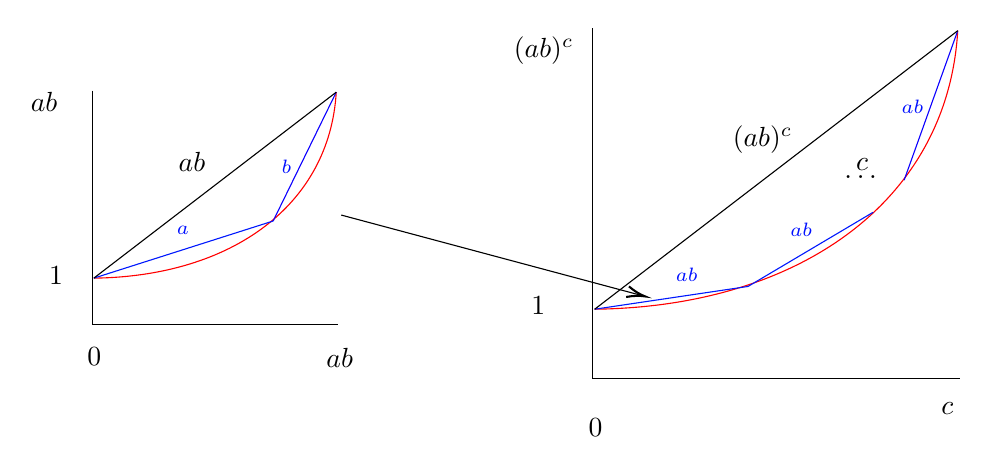
\begin{tikzpicture}[x=0.75pt,y=0.75pt,yscale=-0.8,xscale=0.8]
%uncomment if require: \path (0,300); %set diagram left start at 0, and has height of 300

%Curve Lines [id:da36620019605114806] 
\draw [color={rgb, 255:red, 255; green, 0; blue, 0 }  ,draw opacity=1 ]   (394.15,199.12) .. controls (518.44,197.62) and (606.8,133.23) .. (612.79,31.4) ;
%Straight Lines [id:da02014752812242493] 
\draw    (392.65,241.05) -- (614.28,241.05) ;
%Straight Lines [id:da7970956716447063] 
\draw    (392.65,29.9) -- (392.65,241.05) ;
%Straight Lines [id:da6861214299995879] 
\draw [color={rgb, 255:red, 0; green, 24; blue, 253 }  ,draw opacity=1 ]   (394.15,199.12) -- (486.5,185.41) ;
%Straight Lines [id:da4998942483883625] 
\draw [color={rgb, 255:red, 12; green, 0; blue, 255 }  ,draw opacity=1 ]   (612.79,31.4) -- (580.5,121.41) ;
%Straight Lines [id:da0968150391226873] 
\draw    (394.15,199.12) -- (612.79,31.4) ;
%Straight Lines [id:da5196097062753849] 
\draw [color={rgb, 255:red, 0; green, 24; blue, 253 }  ,draw opacity=1 ]   (486.5,185.41) -- (561.87,140.72) ;
%Curve Lines [id:da9691362275998829] 
\draw [color={rgb, 255:red, 255; green, 0; blue, 0 }  ,draw opacity=1 ]   (92.5,180.41) .. controls (175.5,179.41) and (234.5,136.41) .. (238.5,68.41) ;
%Straight Lines [id:da38041177767308765] 
\draw    (91.5,208.41) -- (239.5,208.41) ;
%Straight Lines [id:da7572437701017198] 
\draw    (91.5,67.41) -- (91.5,208.41) ;
%Straight Lines [id:da5911474121360966] 
\draw [color={rgb, 255:red, 0; green, 24; blue, 253 }  ,draw opacity=1 ]   (92.5,180.41) -- (200.5,146) ;
%Straight Lines [id:da4970471490654107] 
\draw [color={rgb, 255:red, 12; green, 0; blue, 255 }  ,draw opacity=1 ]   (238.5,68.41) -- (200.5,146) ;
%Straight Lines [id:da9854524797466131] 
\draw    (92.5,180.41) -- (238.5,68.41) ;
%Straight Lines [id:da13777115685413477] 
\draw    (241.5,142.41) -- (422.57,190.89) ;
\draw [shift={(424.5,191.41)}, rotate = 194.99] [color={rgb, 255:red, 0; green, 0; blue, 0 }  ][line width=0.75]    (10.93,-3.29) .. controls (6.95,-1.4) and (3.31,-0.3) .. (0,0) .. controls (3.31,0.3) and (6.95,1.4) .. (10.93,3.29)   ;

% Text Node
\draw (388.9,263.4) node [anchor=north west][inner sep=0.75pt]    {$0$};
% Text Node
\draw (601.3,253.9) node [anchor=north west][inner sep=0.75pt]    {$c$};
% Text Node
\draw (354.46,190.02) node [anchor=north west][inner sep=0.75pt]    {$1$};
% Text Node
\draw (475.74,87.19) node [anchor=north west][inner sep=0.75pt]    {$( ab)^{c}$};
% Text Node
\draw (441.49,172.87) node [anchor=north west][inner sep=0.75pt]  [font=\scriptsize,color={rgb, 255:red, 0; green, 15; blue, 255 }  ,opacity=1 ]  {$ab$};
% Text Node
\draw (343.96,33.28) node [anchor=north west][inner sep=0.75pt]    {$( ab)^{c}$};
% Text Node
\draw (543,116.81) node [anchor=north west][inner sep=0.75pt]    {$\dotsc $};
% Text Node
\draw (550,106.81) node [anchor=north west][inner sep=0.75pt]    {$c$};
% Text Node
\draw (510.49,145.87) node [anchor=north west][inner sep=0.75pt]  [font=\scriptsize,color={rgb, 255:red, 0; green, 15; blue, 255 }  ,opacity=1 ]  {$ab$};
% Text Node
\draw (577.49,71.87) node [anchor=north west][inner sep=0.75pt]  [font=\scriptsize,color={rgb, 255:red, 0; green, 15; blue, 255 }  ,opacity=1 ]  {$ab$};
% Text Node
\draw (87,220.81) node [anchor=north west][inner sep=0.75pt]    {$0$};
% Text Node
\draw (231,220.81) node [anchor=north west][inner sep=0.75pt]    {$ab$};
% Text Node
\draw (64,171.81) node [anchor=north west][inner sep=0.75pt]    {$1$};
% Text Node
\draw (142,102.81) node [anchor=north west][inner sep=0.75pt]    {$ab$};
% Text Node
\draw (141,147.81) node [anchor=north west][inner sep=0.75pt]  [font=\scriptsize,color={rgb, 255:red, 0; green, 15; blue, 255 }  ,opacity=1 ]  {$a$};
% Text Node
\draw (204,107.81) node [anchor=north west][inner sep=0.75pt]  [font=\scriptsize,color={rgb, 255:red, 0; green, 15; blue, 255 }  ,opacity=1 ]  {$b$};
% Text Node
\draw (53,66.81) node [anchor=north west][inner sep=0.75pt]    {$ab$};


\end{tikzpicture}

\subsubsection{Logarithm}

If exponentiation measure growth given time,
then the logarithm asks how much time is needed until we grow to a given amount.
Or even better, the amount of time needed to reach a certain proportion of growth.
Take \( b^t \) which measure continuous growth at a proportion of \( b \) per time step
starting at \( t = 0 \) with \( b^t = 1 \).
Then \( \log_b(c) \) is the amount of time needed to reach \( c \).
Thus if \( \log_b(c) = t \), then \( b^t = c \).

\tikzset{every picture/.style={line width=0.75pt}} %set default line width to 0.75pt        

\begin{tikzpicture}[x=0.75pt,y=0.75pt,yscale=-1,xscale=1]
%uncomment if require: \path (0,300); %set diagram left start at 0, and has height of 300

%Curve Lines [id:da44242036711397026] 
\draw [color={rgb, 255:red, 255; green, 0; blue, 0 }  ,draw opacity=1 ]   (135.15,192.12) .. controls (259.44,190.62) and (347.8,126.23) .. (353.79,24.4) ;
%Straight Lines [id:da8686157897249571] 
\draw    (133.65,234.05) -- (355.28,234.05) ;
%Straight Lines [id:da1397224424767859] 
\draw    (133.65,22.9) -- (133.65,234.05) ;
%Shape: Circle [id:dp8600200674827816] 
\draw   (325,106) .. controls (325,104.9) and (325.9,104) .. (327,104) .. controls (328.1,104) and (329,104.9) .. (329,106) .. controls (329,107.1) and (328.1,108) .. (327,108) .. controls (325.9,108) and (325,107.1) .. (325,106) -- cycle ;
%Shape: Circle [id:dp24025383059430205] 
\draw   (221,179) .. controls (221,177.9) and (221.9,177) .. (223,177) .. controls (224.1,177) and (225,177.9) .. (225,179) .. controls (225,180.1) and (224.1,181) .. (223,181) .. controls (221.9,181) and (221,180.1) .. (221,179) -- cycle ;

% Text Node
\draw (129.9,249.4) node [anchor=north west][inner sep=0.75pt]    {$0$};
% Text Node
\draw (103,183.4) node [anchor=north west][inner sep=0.75pt]    {$1$};
% Text Node
\draw (331,109.4) node [anchor=north west][inner sep=0.75pt]    {$c$};
% Text Node
\draw (225,180.4) node [anchor=north west][inner sep=0.75pt]    {$b$};
% Text Node
\draw (221,250.4) node [anchor=north west][inner sep=0.75pt]    {$1$};
% Text Node
\draw (316,248.4) node [anchor=north west][inner sep=0.75pt]    {$\log_{b} \ c$};


\end{tikzpicture}


By this definition, we have \( b^{\log_b(c)} = c \).

For \( \log_b(ac) \),
we can interpret this as the amount of time until we reache a factor of \( ac \).


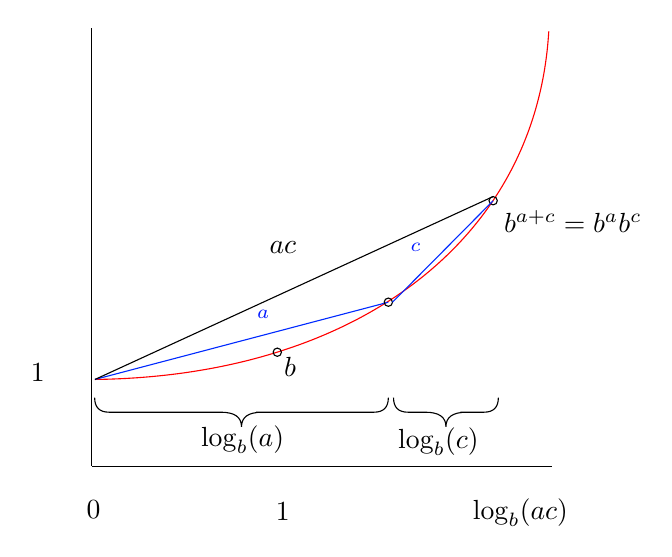
\begin{tikzpicture}[x=0.75pt,y=0.75pt,yscale=-1,xscale=1]
%uncomment if require: \path (0,300); %set diagram left start at 0, and has height of 300

%Curve Lines [id:da03288993175087518] 
\draw [color={rgb, 255:red, 255; green, 0; blue, 0 }  ,draw opacity=1 ]   (155.15,179.22) .. controls (279.44,177.72) and (367.8,113.33) .. (373.79,11.5) ;
%Straight Lines [id:da1130487867315304] 
\draw    (153.65,221.15) -- (375.28,221.15) ;
%Straight Lines [id:da33259651715487903] 
\draw    (153.65,10) -- (153.65,221.15) ;
%Shape: Circle [id:dp08048097645129337] 
\draw   (345,93.1) .. controls (345,91.99) and (345.9,91.1) .. (347,91.1) .. controls (348.1,91.1) and (349,91.99) .. (349,93.1) .. controls (349,94.2) and (348.1,95.1) .. (347,95.1) .. controls (345.9,95.1) and (345,94.2) .. (345,93.1) -- cycle ;
%Shape: Circle [id:dp0349937774727469] 
\draw   (241,166.1) .. controls (241,164.99) and (241.9,164.1) .. (243,164.1) .. controls (244.1,164.1) and (245,164.99) .. (245,166.1) .. controls (245,167.2) and (244.1,168.1) .. (243,168.1) .. controls (241.9,168.1) and (241,167.2) .. (241,166.1) -- cycle ;
%Straight Lines [id:da4023477966991159] 
\draw [color={rgb, 255:red, 0; green, 42; blue, 255 }  ,draw opacity=1 ]   (155.15,179.22) -- (296.5,142) ;
%Shape: Circle [id:dp6857242879889043] 
\draw   (294.5,142) .. controls (294.5,140.9) and (295.4,140) .. (296.5,140) .. controls (297.6,140) and (298.5,140.9) .. (298.5,142) .. controls (298.5,143.1) and (297.6,144) .. (296.5,144) .. controls (295.4,144) and (294.5,143.1) .. (294.5,142) -- cycle ;
%Straight Lines [id:da4161013432719185] 
\draw [color={rgb, 255:red, 0; green, 42; blue, 255 }  ,draw opacity=1 ]   (298.5,142) -- (347,93.1) ;
%Straight Lines [id:da5038115107934119] 
\draw    (155.15,179.22) -- (347,91.1) ;
%Shape: Brace [id:dp5633640978469883] 
\draw   (155,188) .. controls (155,192.67) and (157.33,195) .. (162,195) -- (215.75,195) .. controls (222.42,195) and (225.75,197.33) .. (225.75,202) .. controls (225.75,197.33) and (229.08,195) .. (235.75,195)(232.75,195) -- (289.5,195) .. controls (294.17,195) and (296.5,192.67) .. (296.5,188) ;
%Shape: Brace [id:dp3308211831927511] 
\draw   (299,188) .. controls (299,192.67) and (301.33,195) .. (306,195) -- (314.25,195) .. controls (320.92,195) and (324.25,197.33) .. (324.25,202) .. controls (324.25,197.33) and (327.58,195) .. (334.25,195)(331.25,195) -- (342.5,195) .. controls (347.17,195) and (349.5,192.67) .. (349.5,188) ;

% Text Node
\draw (149.9,236.5) node [anchor=north west][inner sep=0.75pt]    {$0$};
% Text Node
\draw (123,170.5) node [anchor=north west][inner sep=0.75pt]    {$1$};
% Text Node
\draw (351,96.5) node [anchor=north west][inner sep=0.75pt]    {$b^{a+c} =b^{a} b^{c}$};
% Text Node
\draw (245,167.5) node [anchor=north west][inner sep=0.75pt]    {$b$};
% Text Node
\draw (241,237.5) node [anchor=north west][inner sep=0.75pt]    {$1$};
% Text Node
\draw (336,235.5) node [anchor=north west][inner sep=0.75pt]    {$\log_{b}( ac)$};
% Text Node
\draw (232,144.4) node [anchor=north west][inner sep=0.75pt]  [font=\scriptsize,color={rgb, 255:red, 0; green, 24; blue, 255 }  ,opacity=1 ]  {$a$};
% Text Node
\draw (306,112.4) node [anchor=north west][inner sep=0.75pt]  [font=\scriptsize,color={rgb, 255:red, 0; green, 24; blue, 255 }  ,opacity=1 ]  {$c$};
% Text Node
\draw (238,111.4) node [anchor=north west][inner sep=0.75pt]    {$ac$};
% Text Node
\draw (205,200.4) node [anchor=north west][inner sep=0.75pt]    {$\log_{b}( a)$};
% Text Node
\draw (300,201.4) node [anchor=north west][inner sep=0.75pt]    {$\log_{b}( c)$};


\end{tikzpicture}


But since \( ac \) is just \( a \) multiplied by a proportion of \( c \),
we can just find the times for \( b \) and \( c \) separately:
\[ \log_b(ac) = \log_b(a) + \log_b(c). \]

Now for \( log_b(a^c) \),
we want to know the time until we reach a proportion \( a^c \).
We can just figure out the time until \( a \),
then just repeat the time as needed
\[ \log_b(a^c) = c \cdot \log_b(a). \]

\tikzset{every picture/.style={line width=0.75pt}} %set default line width to 0.75pt        

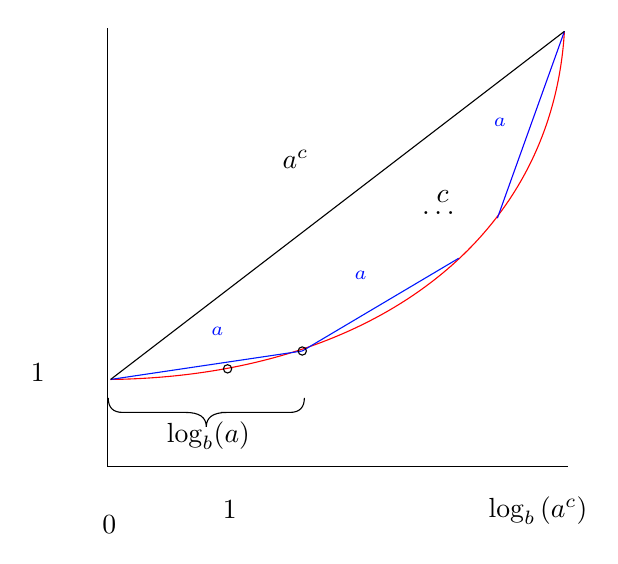
\begin{tikzpicture}[x=0.75pt,y=0.75pt,yscale=-1,xscale=1]
%uncomment if require: \path (0,300); %set diagram left start at 0, and has height of 300

%Curve Lines [id:da5666747848036192] 
\draw [color={rgb, 255:red, 255; green, 0; blue, 0 }  ,draw opacity=1 ]   (141.15,193.12) .. controls (265.44,191.62) and (353.8,127.23) .. (359.79,25.4) ;
%Straight Lines [id:da028560556373229073] 
\draw    (139.65,235.05) -- (361.28,235.05) ;
%Straight Lines [id:da8787938487899625] 
\draw    (139.65,23.9) -- (139.65,235.05) ;
%Straight Lines [id:da788769211427464] 
\draw [color={rgb, 255:red, 0; green, 24; blue, 253 }  ,draw opacity=1 ]   (141.15,193.12) -- (233.5,179.41) ;
%Straight Lines [id:da7332679005966856] 
\draw [color={rgb, 255:red, 12; green, 0; blue, 255 }  ,draw opacity=1 ]   (359.79,25.4) -- (327.5,115.41) ;
%Straight Lines [id:da7194926321605494] 
\draw    (141.15,193.12) -- (359.79,25.4) ;
%Straight Lines [id:da019397101725570853] 
\draw [color={rgb, 255:red, 0; green, 24; blue, 253 }  ,draw opacity=1 ]   (233.5,179.41) -- (308.87,134.72) ;
%Shape: Brace [id:dp6265659815745908] 
\draw   (140,202) .. controls (140,206.67) and (142.33,209) .. (147,209) -- (177.25,209) .. controls (183.92,209) and (187.25,211.33) .. (187.25,216) .. controls (187.25,211.33) and (190.58,209) .. (197.25,209)(194.25,209) -- (227.5,209) .. controls (232.17,209) and (234.5,206.67) .. (234.5,202) ;
%Shape: Circle [id:dp9573621524250069] 
\draw   (231.5,179.41) .. controls (231.5,178.31) and (232.4,177.41) .. (233.5,177.41) .. controls (234.6,177.41) and (235.5,178.31) .. (235.5,179.41) .. controls (235.5,180.51) and (234.6,181.41) .. (233.5,181.41) .. controls (232.4,181.41) and (231.5,180.51) .. (231.5,179.41) -- cycle ;
%Shape: Circle [id:dp3800718490662076] 
\draw   (195.5,188) .. controls (195.5,186.9) and (196.4,186) .. (197.5,186) .. controls (198.6,186) and (199.5,186.9) .. (199.5,188) .. controls (199.5,189.1) and (198.6,190) .. (197.5,190) .. controls (196.4,190) and (195.5,189.1) .. (195.5,188) -- cycle ;

% Text Node
\draw (322,248.5) node [anchor=north west][inner sep=0.75pt]    {$\log_{b}\left( a^{c}\right)$};
% Text Node
\draw (135.9,257.4) node [anchor=north west][inner sep=0.75pt]    {$0$};
% Text Node
\draw (101.46,184.02) node [anchor=north west][inner sep=0.75pt]    {$1$};
% Text Node
\draw (222.74,81.19) node [anchor=north west][inner sep=0.75pt]    {$a^{c}$};
% Text Node
\draw (188.49,166.87) node [anchor=north west][inner sep=0.75pt]  [font=\scriptsize,color={rgb, 255:red, 0; green, 15; blue, 255 }  ,opacity=1 ]  {$a$};
% Text Node
\draw (290,110.81) node [anchor=north west][inner sep=0.75pt]    {$\dotsc $};
% Text Node
\draw (297,100.81) node [anchor=north west][inner sep=0.75pt]    {$c$};
% Text Node
\draw (257.49,139.87) node [anchor=north west][inner sep=0.75pt]  [font=\scriptsize,color={rgb, 255:red, 0; green, 15; blue, 255 }  ,opacity=1 ]  {$a$};
% Text Node
\draw (324.49,65.87) node [anchor=north west][inner sep=0.75pt]  [font=\scriptsize,color={rgb, 255:red, 0; green, 15; blue, 255 }  ,opacity=1 ]  {$a$};
% Text Node
\draw (194,250.4) node [anchor=north west][inner sep=0.75pt]    {$1$};
% Text Node
\draw (167,212.4) node [anchor=north west][inner sep=0.75pt]    {$\log_{b}( a)$};


\end{tikzpicture}

\newpage
We know we can convert between different proportions.

\noindent
\begin{tikzpicture}[x=0.75pt,y=0.75pt,yscale=-0.8,xscale=0.8]
%uncomment if require: \path (0,300); %set diagram left start at 0, and has height of 300

%Curve Lines [id:da31237482832048213] 
\draw [color={rgb, 255:red, 255; green, 0; blue, 0 }  ,draw opacity=1 ]   (57.15,203.12) .. controls (181.44,201.62) and (269.8,137.23) .. (275.79,35.4) ;
%Straight Lines [id:da3926494216948153] 
\draw    (55.65,245.05) -- (277.28,245.05) ;
%Straight Lines [id:da10368000268903799] 
\draw    (55.65,33.9) -- (55.65,245.05) ;
%Shape: Circle [id:dp7976545437139276] 
\draw   (143,190) .. controls (143,188.9) and (143.9,188) .. (145,188) .. controls (146.1,188) and (147,188.9) .. (147,190) .. controls (147,191.1) and (146.1,192) .. (145,192) .. controls (143.9,192) and (143,191.1) .. (143,190) -- cycle ;
%Curve Lines [id:da5946848288292531] 
\draw [color={rgb, 255:red, 255; green, 0; blue, 0 }  ,draw opacity=1 ]   (374.15,206.12) .. controls (498.44,204.62) and (586.8,140.23) .. (592.79,38.4) ;
%Straight Lines [id:da19855608239529243] 
\draw    (372.65,248.05) -- (594.28,248.05) ;
%Straight Lines [id:da6268473981694361] 
\draw    (372.65,36.9) -- (372.65,248.05) ;
%Shape: Circle [id:dp5668748523599273] 
\draw   (558,130) .. controls (558,128.9) and (558.9,128) .. (560,128) .. controls (561.1,128) and (562,128.9) .. (562,130) .. controls (562,131.1) and (561.1,132) .. (560,132) .. controls (558.9,132) and (558,131.1) .. (558,130) -- cycle ;
%Shape: Circle [id:dp3093636342477569] 
\draw   (459,194) .. controls (459,192.9) and (459.9,192) .. (461,192) .. controls (462.1,192) and (463,192.9) .. (463,194) .. controls (463,195.1) and (462.1,196) .. (461,196) .. controls (459.9,196) and (459,195.1) .. (459,194) -- cycle ;
%Straight Lines [id:da9426891179121221] 
\draw [color={rgb, 255:red, 0; green, 15; blue, 255 }  ,draw opacity=1 ]   (461,192) -- (558,130) ;
%Straight Lines [id:da48716811747789657] 
\draw [color={rgb, 255:red, 0; green, 15; blue, 255 }  ,draw opacity=1 ]   (374.15,206.12) -- (459,194) ;
%Straight Lines [id:da1989342802625228] 
\draw    (560,128) -- (374.15,206.12) ;

% Text Node
\draw (51.9,260.4) node [anchor=north west][inner sep=0.75pt]    {$0$};
% Text Node
\draw (25,194.4) node [anchor=north west][inner sep=0.75pt]    {$1$};
% Text Node
\draw (147,191.4) node [anchor=north west][inner sep=0.75pt]    {$b$};
% Text Node
\draw (143,261.4) node [anchor=north west][inner sep=0.75pt]    {$1$};
% Text Node
\draw (368.9,263.4) node [anchor=north west][inner sep=0.75pt]    {$0$};
% Text Node
\draw (342,197.4) node [anchor=north west][inner sep=0.75pt]    {$1$};
% Text Node
\draw (564,133.4) node [anchor=north west][inner sep=0.75pt]    {$a$};
% Text Node
\draw (559,256.4) node [anchor=north west][inner sep=0.75pt]    {$1$};
% Text Node
\draw (130,53.4) node [anchor=north west][inner sep=0.75pt]    {$b^{t}$};
% Text Node
\draw (464,44.4) node [anchor=north west][inner sep=0.75pt]    {$a^{t}$};
% Text Node
\draw (463,199.4) node [anchor=north west][inner sep=0.75pt]    {$b$};


\end{tikzpicture}

Suppose we have \( b^t \) but we want to talk about it in terms of \( a \).
We know the amount of time it takes to reach amount \( b \) at a growth ratio of \( a \)
is \( p = \log_a(b) \).
So \( b^t = a^{pt} \).


\noindent
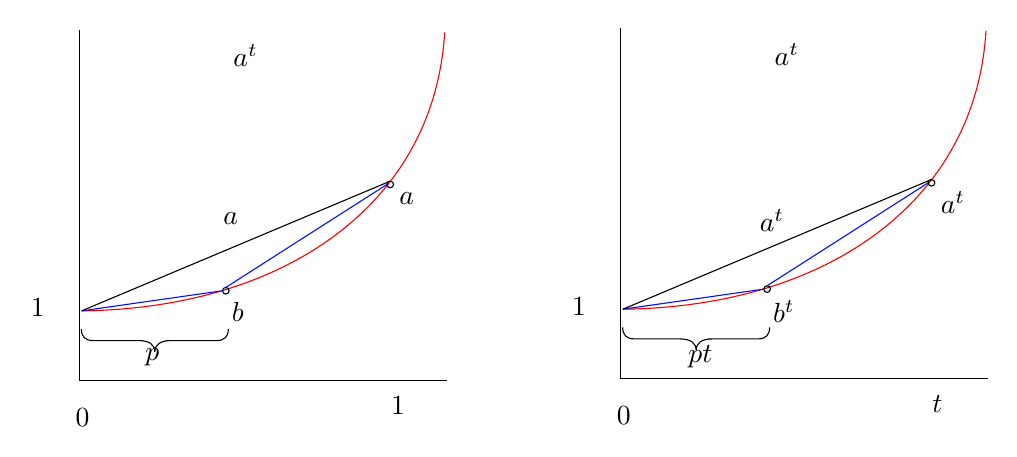
\begin{tikzpicture}[x=0.75pt,y=0.75pt,yscale=-0.8,xscale=0.8]
%uncomment if require: \path (0,300); %set diagram left start at 0, and has height of 300

%Curve Lines [id:da3560394514112394] 
\draw [color={rgb, 255:red, 255; green, 0; blue, 0 }  ,draw opacity=1 ]   (64.15,193.12) .. controls (188.44,191.62) and (276.8,127.23) .. (282.79,25.4) ;
%Straight Lines [id:da9263902741670693] 
\draw    (62.65,235.05) -- (284.28,235.05) ;
%Straight Lines [id:da2728997473938879] 
\draw    (62.65,23.9) -- (62.65,235.05) ;
%Shape: Circle [id:dp9589136983599007] 
\draw   (248,117) .. controls (248,115.9) and (248.9,115) .. (250,115) .. controls (251.1,115) and (252,115.9) .. (252,117) .. controls (252,118.1) and (251.1,119) .. (250,119) .. controls (248.9,119) and (248,118.1) .. (248,117) -- cycle ;
%Shape: Circle [id:dp6864610263532174] 
\draw   (149,181) .. controls (149,179.9) and (149.9,179) .. (151,179) .. controls (152.1,179) and (153,179.9) .. (153,181) .. controls (153,182.1) and (152.1,183) .. (151,183) .. controls (149.9,183) and (149,182.1) .. (149,181) -- cycle ;
%Straight Lines [id:da8490675899505665] 
\draw [color={rgb, 255:red, 0; green, 15; blue, 255 }  ,draw opacity=1 ]   (151,179) -- (248,117) ;
%Straight Lines [id:da7420557649919006] 
\draw [color={rgb, 255:red, 0; green, 15; blue, 255 }  ,draw opacity=1 ]   (64.15,193.12) -- (149,181) ;
%Straight Lines [id:da22009305504529253] 
\draw    (250,115) -- (64.15,193.12) ;
%Shape: Brace [id:dp4270781839595835] 
\draw   (64,204) .. controls (64,208.67) and (66.33,211) .. (71,211) -- (98.25,211) .. controls (104.92,211) and (108.25,213.33) .. (108.25,218) .. controls (108.25,213.33) and (111.58,211) .. (118.25,211)(115.25,211) -- (145.5,211) .. controls (150.17,211) and (152.5,208.67) .. (152.5,204) ;
%Curve Lines [id:da0579876890242087] 
\draw [color={rgb, 255:red, 255; green, 0; blue, 0 }  ,draw opacity=1 ]   (390.15,192.12) .. controls (514.44,190.62) and (602.8,126.23) .. (608.79,24.4) ;
%Straight Lines [id:da052635434270711046] 
\draw    (388.65,234.05) -- (610.28,234.05) ;
%Straight Lines [id:da0009454214185438126] 
\draw    (388.65,22.9) -- (388.65,234.05) ;
%Shape: Circle [id:dp9197894858730317] 
\draw   (574,116) .. controls (574,114.9) and (574.9,114) .. (576,114) .. controls (577.1,114) and (578,114.9) .. (578,116) .. controls (578,117.1) and (577.1,118) .. (576,118) .. controls (574.9,118) and (574,117.1) .. (574,116) -- cycle ;
%Shape: Circle [id:dp2623475297033576] 
\draw   (475,180) .. controls (475,178.9) and (475.9,178) .. (477,178) .. controls (478.1,178) and (479,178.9) .. (479,180) .. controls (479,181.1) and (478.1,182) .. (477,182) .. controls (475.9,182) and (475,181.1) .. (475,180) -- cycle ;
%Straight Lines [id:da7991503677748758] 
\draw [color={rgb, 255:red, 0; green, 15; blue, 255 }  ,draw opacity=1 ]   (477,178) -- (574,116) ;
%Straight Lines [id:da1905041719331747] 
\draw [color={rgb, 255:red, 0; green, 15; blue, 255 }  ,draw opacity=1 ]   (390.15,192.12) -- (475,180) ;
%Straight Lines [id:da5956130209216697] 
\draw    (576,114) -- (390.15,192.12) ;
%Shape: Brace [id:dp2030184487810177] 
\draw   (390,203) .. controls (390,207.67) and (392.33,210) .. (397,210) -- (424.25,210) .. controls (430.92,210) and (434.25,212.33) .. (434.25,217) .. controls (434.25,212.33) and (437.58,210) .. (444.25,210)(441.25,210) -- (471.5,210) .. controls (476.17,210) and (478.5,207.67) .. (478.5,203) ;

% Text Node
\draw (58.9,250.4) node [anchor=north west][inner sep=0.75pt]    {$0$};
% Text Node
\draw (32,184.4) node [anchor=north west][inner sep=0.75pt]    {$1$};
% Text Node
\draw (254,120.4) node [anchor=north west][inner sep=0.75pt]    {$a$};
% Text Node
\draw (249,243.4) node [anchor=north west][inner sep=0.75pt]    {$1$};
% Text Node
\draw (154,31.4) node [anchor=north west][inner sep=0.75pt]    {$a^{t}$};
% Text Node
\draw (153,186.4) node [anchor=north west][inner sep=0.75pt]    {$b$};
% Text Node
\draw (101,214.4) node [anchor=north west][inner sep=0.75pt]    {$p$};
% Text Node
\draw (384.9,249.4) node [anchor=north west][inner sep=0.75pt]    {$0$};
% Text Node
\draw (358,183.4) node [anchor=north west][inner sep=0.75pt]    {$1$};
% Text Node
\draw (580,119.4) node [anchor=north west][inner sep=0.75pt]    {$a^{t}$};
% Text Node
\draw (575,242.4) node [anchor=north west][inner sep=0.75pt]    {$t$};
% Text Node
\draw (480,30.4) node [anchor=north west][inner sep=0.75pt]    {$a^{t}$};
% Text Node
\draw (479,185.4) node [anchor=north west][inner sep=0.75pt]    {$b^{t}$};
% Text Node
\draw (428,212.4) node [anchor=north west][inner sep=0.75pt]    {$pt$};
% Text Node
\draw (148,132.4) node [anchor=north west][inner sep=0.75pt]    {$a$};
% Text Node
\draw (471,130.4) node [anchor=north west][inner sep=0.75pt]    {$a^{t}$};


\end{tikzpicture}

And \( \log_a(b^t) = t \cdot \log_a(b) \), and \( t = \frac{\log_a(b^t)}{\log_a(b)} \).


\begin{tikzpicture}[x=0.75pt,y=0.75pt,yscale=-1,xscale=1]
%uncomment if require: \path (0,300); %set diagram left start at 0, and has height of 300

%Curve Lines [id:da4423317108802115] 
\draw [color={rgb, 255:red, 255; green, 0; blue, 0 }  ,draw opacity=1 ]   (77.15,205.12) .. controls (201.44,203.62) and (289.8,139.23) .. (295.79,37.4) ;
%Straight Lines [id:da9534342452823479] 
\draw    (75.65,247.05) -- (297.28,247.05) ;
%Straight Lines [id:da33389606852560494] 
\draw    (75.65,35.9) -- (75.65,247.05) ;
%Shape: Circle [id:dp26393026690295507] 
\draw   (163,192) .. controls (163,190.9) and (163.9,190) .. (165,190) .. controls (166.1,190) and (167,190.9) .. (167,192) .. controls (167,193.1) and (166.1,194) .. (165,194) .. controls (163.9,194) and (163,193.1) .. (163,192) -- cycle ;
%Shape: Circle [id:dp10820914245059055] 
\draw   (123,201) .. controls (123,199.9) and (123.9,199) .. (125,199) .. controls (126.1,199) and (127,199.9) .. (127,201) .. controls (127,202.1) and (126.1,203) .. (125,203) .. controls (123.9,203) and (123,202.1) .. (123,201) -- cycle ;
%Shape: Circle [id:dp5803203757563192] 
\draw   (202,176) .. controls (202,174.9) and (202.9,174) .. (204,174) .. controls (205.1,174) and (206,174.9) .. (206,176) .. controls (206,177.1) and (205.1,178) .. (204,178) .. controls (202.9,178) and (202,177.1) .. (202,176) -- cycle ;
%Shape: Circle [id:dp5182181490141611] 
\draw   (255,137) .. controls (255,135.9) and (255.9,135) .. (257,135) .. controls (258.1,135) and (259,135.9) .. (259,137) .. controls (259,138.1) and (258.1,139) .. (257,139) .. controls (255.9,139) and (255,138.1) .. (255,137) -- cycle ;

% Text Node
\draw (71.9,262.4) node [anchor=north west][inner sep=0.75pt]    {$0$};
% Text Node
\draw (45,196.4) node [anchor=north west][inner sep=0.75pt]    {$1$};
% Text Node
\draw (167,193.4) node [anchor=north west][inner sep=0.75pt]  [color={rgb, 255:red, 255; green, 0; blue, 4 }  ,opacity=1 ]  {$e$};
% Text Node
\draw (163,263.4) node [anchor=north west][inner sep=0.75pt]    {$1$};
% Text Node
\draw (150,55.4) node [anchor=north west][inner sep=0.75pt]    {$e^{t}$};
% Text Node
\draw (127,202.4) node [anchor=north west][inner sep=0.75pt]    {$a$};
% Text Node
\draw (208,179.4) node [anchor=north west][inner sep=0.75pt]    {$b$};
% Text Node
\draw (261,140.4) node [anchor=north west][inner sep=0.75pt]    {$c$};


\end{tikzpicture}

So \( \log \) is just a measurement, but in terms of the length of 1
which is just the length until we reach a proportion of the base.
Since all exponential functions are really the same,
we can just think of them all in terms of a common base, say \( e \).
Then our measuring stick of 1 is just \( \ln(e) = 1\).

So if we are given \( \log_a(x) \), this just means
the length until we reach a multiple of \( x \),
but measured if 1 was the length until \( a \).
Thus \( \log_a(x) = \frac{\ln(x)}{\ln(a)} \).


\newpage
\section{Functions}

\subsection{Linear Functions}

A linear function \( f(x) = cx \) is a constant scaling.
It has the properties that it maps 0 to 0,
that it preserves addition: \( f(a+b) = f(a) + f(b) \),
and that it preserves additional scaling: \( f(cx) = cf(x) \).
This results in something like the real line being mapped to an evenly spaced out line.
The scaling constant \( c \) is the slope.

\tikzset{every picture/.style={line width=0.75pt}} %set default line width to 0.75pt        

\begin{tikzpicture}[x=0.75pt,y=0.75pt,yscale=-0.9,xscale=0.9]
%uncomment if require: \path (0,300); %set diagram left start at 0, and has height of 300

%Straight Lines [id:da25462787180907864] 
\draw    (237.5,129) -- (426.5,129) ;
%Straight Lines [id:da9265458358278599] 
\draw    (332.5,122) -- (332.5,135) ;
%Straight Lines [id:da4937452292425144] 
\draw    (352.5,122) -- (352.5,135) ;
%Straight Lines [id:da37252610433795874] 
\draw    (371.5,124) -- (371.5,137) ;
%Straight Lines [id:da8047296850692236] 
\draw    (392.5,124) -- (392.5,137) ;
%Straight Lines [id:da776603621592167] 
\draw    (409.5,124) -- (409.5,137) ;
%Straight Lines [id:da8193752468395039] 
\draw    (254.5,121) -- (254.5,134) ;
%Straight Lines [id:da3301411605586583] 
\draw    (273.5,123) -- (273.5,136) ;
%Straight Lines [id:da2678642381996833] 
\draw    (294.5,123) -- (294.5,136) ;
%Straight Lines [id:da6613938456603193] 
\draw    (311.5,123) -- (311.5,136) ;
%Straight Lines [id:da927602811346756] 
\draw    (80.5,213) -- (580.5,213) ;
%Straight Lines [id:da5881278384912296] 
\draw    (331.82,206) -- (331.82,219) ;
%Straight Lines [id:da5456376454630552] 
\draw    (384.73,206) -- (384.73,219) ;
%Straight Lines [id:da3510407939296091] 
\draw    (435,208) -- (435,221) ;
%Straight Lines [id:da16761479489048103] 
\draw    (490.55,208) -- (490.55,221) ;
%Straight Lines [id:da4375264334043748] 
\draw    (535.53,208) -- (535.53,221) ;
%Straight Lines [id:da09028825711730781] 
\draw    (125.47,205) -- (125.47,218) ;
%Straight Lines [id:da9169436778878468] 
\draw    (175.74,207) -- (175.74,220) ;
%Straight Lines [id:da2383948835059787] 
\draw    (231.29,207) -- (231.29,220) ;
%Straight Lines [id:da24685243888466935] 
\draw    (276.27,207) -- (276.27,220) ;

% Text Node
\draw (326,96.4) node [anchor=north west][inner sep=0.75pt]    {$0$};
% Text Node
\draw (326,178.4) node [anchor=north west][inner sep=0.75pt]    {$0$};
% Text Node
\draw (317,147.4) node [anchor=north west][inner sep=0.75pt]    {$f\downarrow $};


\end{tikzpicture}

Translations of linear functions are called affine functions.

\subsection{Composition}

Think of \( f(2x) \) as running through the function twice as fast.
Think of \( f(x + 2) \) as starting running through the function at 2.
Given some \( g(x) \), we can think of \( f(g(x)) \)
where the rate we are running through \( f \) is determined by \( g(x) \).

\subsection{Change of Variables}

Consider \( f(x) = x\).
What do we really mean by this?
One way we can interpret it is to think about \( f \) \emph{with respect to} \( x \).
That is, for every value of \( x \), what does \( f \) map \( x \) to?
But what do we mean by \( x \)?
How should we think about it?

One way is to think about \( x \)
as an arbitrary measure of something,
and that \( f \) assigns a value to each measurement.
In the usual case,
we can think of \( x \) as a short hand for the identity function, \( I(x) \)
on the reals.
In this case, \( I \) just measures the real line as is.
But what about an arbitrary measure functions such as \( g(x) = 2x \)?
Then \( f(2x) = f(g(x)) \) and now we are talking about \( f \) with respect to \( g \).
That is, for each value of \( g \), what is it mapped to by \( f \)?

The standard way to present a function visually is to draw two axes.
We use the vertical axis to represent the value of a function,
and we use the horizontal axis to represent
whatever it is we are valuing the function in terms of.
We normally use each axis to represent the real numbers,
but we can use the horizontal for example to represent the values of \( g(x) \).
Spacing out each axis equally and regularly, we can draw our function \( f(g(x)) \):

\tikzset{every picture/.style={line width=0.75pt}} %set default line width to 0.75pt        

\begin{tikzpicture}[x=0.75pt,y=0.75pt,yscale=-1,xscale=1]
%uncomment if require: \path (0,300); %set diagram left start at 0, and has height of 300

%Shape: Axis 2D [id:dp5189031050967029] 
\draw  (138.5,253.6) -- (476.5,253.6)(172.3,43) -- (172.3,277) (469.5,248.6) -- (476.5,253.6) -- (469.5,258.6) (167.3,50) -- (172.3,43) -- (177.3,50) (232.3,248.6) -- (232.3,258.6)(292.3,248.6) -- (292.3,258.6)(352.3,248.6) -- (352.3,258.6)(412.3,248.6) -- (412.3,258.6)(167.3,193.6) -- (177.3,193.6)(167.3,133.6) -- (177.3,133.6)(167.3,73.6) -- (177.3,73.6) ;
\draw   ;
%Shape: Grid [id:dp9709588135168393] 
\draw  [draw opacity=0] (172.3,73.3) -- (472.3,73.3) -- (472.3,253.3) -- (172.3,253.3) -- cycle ; \draw  [color={rgb, 255:red, 0; green, 0; blue, 0 }  ,draw opacity=0.27 ] (232.3,73.3) -- (232.3,253.3)(292.3,73.3) -- (292.3,253.3)(352.3,73.3) -- (352.3,253.3)(412.3,73.3) -- (412.3,253.3) ; \draw  [color={rgb, 255:red, 0; green, 0; blue, 0 }  ,draw opacity=0.27 ] (172.3,133.3) -- (472.3,133.3)(172.3,193.3) -- (472.3,193.3) ; \draw  [color={rgb, 255:red, 0; green, 0; blue, 0 }  ,draw opacity=0.27 ] (172.3,73.3) -- (472.3,73.3) -- (472.3,253.3) -- (172.3,253.3) -- cycle ;
%Straight Lines [id:da7269112675901455] 
\draw    (172.3,253.3) -- (352.3,73.3) ;

% Text Node
\draw (152,7.4) node [anchor=north west][inner sep=0.75pt]    {$f( g( x))$};
% Text Node
\draw (484,244.4) node [anchor=north west][inner sep=0.75pt]    {$g( x)$};


\end{tikzpicture}

Since \( f(x) = x \),
when \( g(x) = a \), we have \( f(a) = a \).
Note that \( x \) is being used two different ways here,
first just as a variable, and second, as \( I(x) \).
Another way to think about this graph is it to think about the graph of \( g \),
and imagine using the vertical axis as the new horizontal axis for the graph of \( f \).

But now what if we want to talk about \( f \circ g \) with respect to \( x \)?
We now have to translate from the reals to \( g(x) \)
before we can talk about the values of \( f \).


\subsection{Graphs}

A real function is a single dimensional measurement of quantity.
With one variable, the quantity is parameterized in one dimension by the input.
In other words, as we vary the input dimension, what do we get in the output dimension?
We can graph this relationship as such.

\tikzset{every picture/.style={line width=0.75pt}} %set default line width to 0.75pt        

\begin{tikzpicture}[x=0.75pt,y=0.75pt,yscale=-1,xscale=1]
%uncomment if require: \path (0,300); %set diagram left start at 0, and has height of 300

%Shape: Axis 2D [id:dp7522167816409159] 
\draw  (50,242) -- (419.5,242)(97.5,8) -- (97.5,267) (412.5,237) -- (419.5,242) -- (412.5,247) (92.5,15) -- (97.5,8) -- (102.5,15) (146.5,237) -- (146.5,247)(195.5,237) -- (195.5,247)(244.5,237) -- (244.5,247)(293.5,237) -- (293.5,247)(342.5,237) -- (342.5,247)(391.5,237) -- (391.5,247)(92.5,193) -- (102.5,193)(92.5,144) -- (102.5,144)(92.5,95) -- (102.5,95)(92.5,46) -- (102.5,46) ;
\draw   ;
%Shape: Circle [id:dp1800333897763694] 
\draw   (297,120.75) .. controls (297,117.57) and (299.57,115) .. (302.75,115) .. controls (305.93,115) and (308.5,117.57) .. (308.5,120.75) .. controls (308.5,123.93) and (305.93,126.5) .. (302.75,126.5) .. controls (299.57,126.5) and (297,123.93) .. (297,120.75) -- cycle ;
%Curve Lines [id:da6744184215507455] 
\draw    (98,171) .. controls (107.79,163.66) and (111.03,107.89) .. (139.27,154.95) .. controls (167.5,202) and (206.02,160.39) .. (242.5,187) .. controls (278.98,213.61) and (267.5,117) .. (297,120.75) ;
%Straight Lines [id:da042236632067626734] 
\draw [color={rgb, 255:red, 255; green, 0; blue, 0 }  ,draw opacity=1 ]   (302,103) -- (302,62) ;
\draw [shift={(302,60)}, rotate = 450] [color={rgb, 255:red, 255; green, 0; blue, 0 }  ,draw opacity=1 ][line width=0.75]    (10.93,-3.29) .. controls (6.95,-1.4) and (3.31,-0.3) .. (0,0) .. controls (3.31,0.3) and (6.95,1.4) .. (10.93,3.29)   ;
%Straight Lines [id:da8879089279998805] 
\draw [color={rgb, 255:red, 255; green, 0; blue, 0 }  ,draw opacity=1 ]   (301.75,136.5) -- (301.75,175) ;
\draw [shift={(301.75,177)}, rotate = 270] [color={rgb, 255:red, 255; green, 0; blue, 0 }  ,draw opacity=1 ][line width=0.75]    (10.93,-3.29) .. controls (6.95,-1.4) and (3.31,-0.3) .. (0,0) .. controls (3.31,0.3) and (6.95,1.4) .. (10.93,3.29)   ;
%Straight Lines [id:da984234265425485] 
\draw  [dash pattern={on 0.84pt off 2.51pt}]  (302.75,126.5) -- (302.75,245) ;
%Straight Lines [id:da851126430686476] 
\draw [color={rgb, 255:red, 0; green, 42; blue, 255 }  ,draw opacity=1 ]   (267,260) -- (298.5,260) ;
\draw [shift={(300.5,260)}, rotate = 180] [color={rgb, 255:red, 0; green, 42; blue, 255 }  ,draw opacity=1 ][line width=0.75]    (10.93,-3.29) .. controls (6.95,-1.4) and (3.31,-0.3) .. (0,0) .. controls (3.31,0.3) and (6.95,1.4) .. (10.93,3.29)   ;


\end{tikzpicture}


We don't care about the location of the "ball", we only care about the height.


\subsection{Inverse}

For an invertible \( f \), we have \( f\inv \).
Imagine turning the graph of \( f \) counterclockwise.

\tikzset{every picture/.style={line width=0.75pt}} %set default line width to 0.75pt        
\noindent
\begin{tikzpicture}[x=0.75pt,y=0.75pt,yscale=-1,xscale=1]
%uncomment if require: \path (0,300); %set diagram left start at 0, and has height of 300

%Shape: Axis 2D [id:dp7548955269279164] 
\draw  (34,249) -- (327.5,249)(71.73,15) -- (71.73,274) (320.5,244) -- (327.5,249) -- (320.5,254) (66.73,22) -- (71.73,15) -- (76.73,22) (120.73,244) -- (120.73,254)(169.73,244) -- (169.73,254)(218.73,244) -- (218.73,254)(267.73,244) -- (267.73,254)(66.73,200) -- (76.73,200)(66.73,151) -- (76.73,151)(66.73,102) -- (76.73,102)(66.73,53) -- (76.73,53) ;
\draw   ;
%Shape: Circle [id:dp591863864638757] 
\draw   (270,96.75) .. controls (270,93.57) and (272.57,91) .. (275.75,91) .. controls (278.93,91) and (281.5,93.57) .. (281.5,96.75) .. controls (281.5,99.93) and (278.93,102.5) .. (275.75,102.5) .. controls (272.57,102.5) and (270,99.93) .. (270,96.75) -- cycle ;
%Curve Lines [id:da9965257383628019] 
\draw    (71.73,249) .. controls (91.23,242) and (75.5,211) .. (112.5,194) .. controls (149.5,177) and (180.5,189) .. (207.5,163) .. controls (234.5,137) and (243.5,104) .. (270,96.75) ;
%Straight Lines [id:da4442636779784198] 
\draw [color={rgb, 255:red, 255; green, 0; blue, 0 }  ,draw opacity=1 ]   (275,79) -- (275,38) ;
\draw [shift={(275,36)}, rotate = 450] [color={rgb, 255:red, 255; green, 0; blue, 0 }  ,draw opacity=1 ][line width=0.75]    (10.93,-3.29) .. controls (6.95,-1.4) and (3.31,-0.3) .. (0,0) .. controls (3.31,0.3) and (6.95,1.4) .. (10.93,3.29)   ;
%Straight Lines [id:da7277065515801376] 
\draw [color={rgb, 255:red, 255; green, 0; blue, 0 }  ,draw opacity=1 ]   (274.75,112.5) -- (274.75,151) ;
\draw [shift={(274.75,153)}, rotate = 270] [color={rgb, 255:red, 255; green, 0; blue, 0 }  ,draw opacity=1 ][line width=0.75]    (10.93,-3.29) .. controls (6.95,-1.4) and (3.31,-0.3) .. (0,0) .. controls (3.31,0.3) and (6.95,1.4) .. (10.93,3.29)   ;
%Straight Lines [id:da9297137452591817] 
\draw  [dash pattern={on 0.84pt off 2.51pt}]  (275.75,102.5) -- (275.75,249) ;
%Straight Lines [id:da19635560871451874] 
\draw [color={rgb, 255:red, 0; green, 42; blue, 255 }  ,draw opacity=1 ]   (241,272) -- (272.5,272) ;
\draw [shift={(274.5,272)}, rotate = 180] [color={rgb, 255:red, 0; green, 42; blue, 255 }  ,draw opacity=1 ][line width=0.75]    (10.93,-3.29) .. controls (6.95,-1.4) and (3.31,-0.3) .. (0,0) .. controls (3.31,0.3) and (6.95,1.4) .. (10.93,3.29)   ;
%Shape: Axis 2D [id:dp5159473195200954] 
\draw  (587.2,287.9) -- (587.3,-5.6)(353.21,250.09) -- (612.21,250.18) (582.3,1.4) -- (587.3,-5.6) -- (592.3,1.4) (360.21,255.09) -- (353.21,250.09) -- (360.21,245.09) (582.23,201.17) -- (592.23,201.17)(582.25,152.17) -- (592.25,152.17)(582.26,103.17) -- (592.26,103.17)(582.28,54.17) -- (592.28,54.17)(538.21,255.15) -- (538.21,245.15)(489.21,255.13) -- (489.21,245.13)(440.21,255.12) -- (440.21,245.12)(391.21,255.1) -- (391.21,245.1) ;
\draw   ;
%Shape: Circle [id:dp3595956560062188] 
\draw   (435.03,51.85) .. controls (431.86,51.84) and (429.28,49.27) .. (429.28,46.09) .. controls (429.28,42.92) and (431.86,40.34) .. (435.03,40.35) .. controls (438.21,40.35) and (440.78,42.92) .. (440.78,46.1) .. controls (440.78,49.27) and (438.21,51.85) .. (435.03,51.85) -- cycle ;
%Curve Lines [id:da5301486307360965] 
\draw    (587.21,250.17) .. controls (580.22,230.67) and (549.21,246.39) .. (532.23,209.38) .. controls (515.24,172.37) and (527.25,141.38) .. (501.26,114.37) .. controls (475.27,87.36) and (442.27,78.35) .. (435.03,51.85) ;
%Straight Lines [id:da1701708037395353] 
\draw [color={rgb, 255:red, 255; green, 0; blue, 0 }  ,draw opacity=1 ]   (417.28,46.84) -- (376.28,46.83) ;
\draw [shift={(374.28,46.82)}, rotate = 360.02] [color={rgb, 255:red, 255; green, 0; blue, 0 }  ,draw opacity=1 ][line width=0.75]    (10.93,-3.29) .. controls (6.95,-1.4) and (3.31,-0.3) .. (0,0) .. controls (3.31,0.3) and (6.95,1.4) .. (10.93,3.29)   ;
%Straight Lines [id:da9454232351703403] 
\draw [color={rgb, 255:red, 255; green, 0; blue, 0 }  ,draw opacity=1 ]   (450.78,47.1) -- (489.28,47.12) ;
\draw [shift={(491.28,47.12)}, rotate = 180.02] [color={rgb, 255:red, 255; green, 0; blue, 0 }  ,draw opacity=1 ][line width=0.75]    (10.93,-3.29) .. controls (6.95,-1.4) and (3.31,-0.3) .. (0,0) .. controls (3.31,0.3) and (6.95,1.4) .. (10.93,3.29)   ;
%Straight Lines [id:da6128160114394268] 
\draw  [dash pattern={on 0.84pt off 2.51pt}]  (440.78,46.1) -- (587.28,46.15) ;
%Straight Lines [id:da5100793300598488] 
\draw [color={rgb, 255:red, 0; green, 42; blue, 255 }  ,draw opacity=1 ]   (610.27,80.91) -- (610.28,49.41) ;
\draw [shift={(610.28,47.41)}, rotate = 450.02] [color={rgb, 255:red, 0; green, 42; blue, 255 }  ,draw opacity=1 ][line width=0.75]    (10.93,-3.29) .. controls (6.95,-1.4) and (3.31,-0.3) .. (0,0) .. controls (3.31,0.3) and (6.95,1.4) .. (10.93,3.29)   ;
%Curve Lines [id:da5319468231161516] 
\draw    (367.5,35) .. controls (366.51,-6.58) and (296.91,-9.94) .. (291.64,34.63) ;
\draw [shift={(291.5,36)}, rotate = 274.97] [color={rgb, 255:red, 0; green, 0; blue, 0 }  ][line width=0.75]    (10.93,-3.29) .. controls (6.95,-1.4) and (3.31,-0.3) .. (0,0) .. controls (3.31,0.3) and (6.95,1.4) .. (10.93,3.29)   ;

% Text Node
\draw (28,124.4) node [anchor=north west][inner sep=0.75pt]    {$f$};
% Text Node
\draw (161,261.4) node [anchor=north west][inner sep=0.75pt]    {$x$};
% Text Node
\draw (462.6,293.86) node [anchor=north west][inner sep=0.75pt]  [rotate=-270.02]  {$f$};
% Text Node
\draw (599.64,160.9) node [anchor=north west][inner sep=0.75pt]  [rotate=-270.02]  {$x$};


\end{tikzpicture}

Then the inverse function is what we get if we try to stretch the vertical axis
in order to get a straight line.

\tikzset{every picture/.style={line width=0.75pt}} %set default line width to 0.75pt        
\noindent
\begin{tikzpicture}[x=0.75pt,y=0.75pt,yscale=-1,xscale=1]
%uncomment if require: \path (0,300); %set diagram left start at 0, and has height of 300

%Shape: Axis 2D [id:dp5929370070497932] 
\draw  (559.5,300.66) -- (560.68,7.16)(325.65,261.99) -- (584.65,263.03) (555.65,14.14) -- (560.68,7.16) -- (565.65,14.18) (332.63,267.02) -- (325.65,261.99) -- (332.67,257.02) (554.85,213.91) -- (564.85,213.95)(555.04,164.91) -- (565.04,164.95)(555.24,115.91) -- (565.24,115.95)(555.44,66.91) -- (565.44,66.95)(510.63,267.73) -- (510.67,257.73)(461.63,267.54) -- (461.67,257.54)(412.63,267.34) -- (412.67,257.34)(363.63,267.14) -- (363.67,257.14) ;
\draw   ;
%Shape: Circle [id:dp2922848487759444] 
\draw   (367.48,76.53) .. controls (364.3,76.52) and (361.74,73.93) .. (361.75,70.76) .. controls (361.76,67.58) and (364.35,65.02) .. (367.52,65.03) .. controls (370.7,65.04) and (373.26,67.63) .. (373.25,70.8) .. controls (373.24,73.98) and (370.65,76.54) .. (367.48,76.53) -- cycle ;
%Straight Lines [id:da4460470746702786] 
\draw [color={rgb, 255:red, 255; green, 0; blue, 0 }  ,draw opacity=1 ]   (366.47,56.98) -- (366.47,27) ;
\draw [shift={(366.47,25)}, rotate = 450] [color={rgb, 255:red, 255; green, 0; blue, 0 }  ,draw opacity=1 ][line width=0.75]    (10.93,-3.29) .. controls (6.95,-1.4) and (3.31,-0.3) .. (0,0) .. controls (3.31,0.3) and (6.95,1.4) .. (10.93,3.29)   ;
%Straight Lines [id:da7664015619288688] 
\draw [color={rgb, 255:red, 255; green, 0; blue, 0 }  ,draw opacity=1 ]   (366.97,89.36) -- (366.97,120) ;
\draw [shift={(366.97,122)}, rotate = 270] [color={rgb, 255:red, 255; green, 0; blue, 0 }  ,draw opacity=1 ][line width=0.75]    (10.93,-3.29) .. controls (6.95,-1.4) and (3.31,-0.3) .. (0,0) .. controls (3.31,0.3) and (6.95,1.4) .. (10.93,3.29)   ;
%Straight Lines [id:da26802888705480965] 
\draw  [dash pattern={on 0.84pt off 2.51pt}]  (366.97,89.36) -- (366.97,262) ;
%Straight Lines [id:da7801033298249271] 
\draw [color={rgb, 255:red, 0; green, 42; blue, 255 }  ,draw opacity=1 ]   (407.33,284.75) -- (369.5,284.75) ;
\draw [shift={(367.5,284.75)}, rotate = 360] [color={rgb, 255:red, 0; green, 42; blue, 255 }  ,draw opacity=1 ][line width=0.75]    (10.93,-3.29) .. controls (6.95,-1.4) and (3.31,-0.3) .. (0,0) .. controls (3.31,0.3) and (6.95,1.4) .. (10.93,3.29)   ;
%Straight Lines [id:da18575964657480493] 
\draw    (372.5,75.78) -- (559.65,262.93) ;
%Shape: Axis 2D [id:dp6183296547401036] 
\draw  (251.02,291.7) -- (249.44,-1.8)(16.82,255.23) -- (275.82,253.83) (244.47,5.23) -- (249.44,-1.8) -- (254.47,5.17) (23.85,260.19) -- (16.82,255.23) -- (23.8,250.19) (245.55,204.99) -- (255.55,204.94)(245.29,156) -- (255.29,155.94)(245.02,107) -- (255.02,106.94)(244.76,58) -- (254.76,57.94)(201.85,259.23) -- (201.79,249.23)(152.85,259.5) -- (152.79,249.5)(103.85,259.76) -- (103.79,249.76)(54.85,260.03) -- (54.8,250.03) ;
\draw   ;
%Shape: Circle [id:dp5469452186008116] 
\draw   (97.5,56.52) .. controls (94.32,56.54) and (91.74,53.98) .. (91.72,50.8) .. controls (91.7,47.63) and (94.26,45.04) .. (97.44,45.02) .. controls (100.61,45.01) and (103.2,47.57) .. (103.22,50.74) .. controls (103.23,53.92) and (100.67,56.51) .. (97.5,56.52) -- cycle ;
%Curve Lines [id:da8871726471746693] 
\draw    (250.82,253.97) .. controls (243.71,234.5) and (212.8,250.4) .. (195.6,213.49) .. controls (178.4,176.59) and (190.23,145.52) .. (164.09,118.66) .. controls (137.94,91.8) and (104.89,82.98) .. (97.5,56.52) ;
%Straight Lines [id:da5533004496996091] 
\draw [color={rgb, 255:red, 255; green, 0; blue, 0 }  ,draw opacity=1 ]   (79.72,51.62) -- (38.72,51.84) ;
\draw [shift={(36.72,51.85)}, rotate = 359.69] [color={rgb, 255:red, 255; green, 0; blue, 0 }  ,draw opacity=1 ][line width=0.75]    (10.93,-3.29) .. controls (6.95,-1.4) and (3.31,-0.3) .. (0,0) .. controls (3.31,0.3) and (6.95,1.4) .. (10.93,3.29)   ;
%Straight Lines [id:da9787473715679051] 
\draw [color={rgb, 255:red, 255; green, 0; blue, 0 }  ,draw opacity=1 ]   (113.22,51.69) -- (151.72,51.48) ;
\draw [shift={(153.72,51.47)}, rotate = 539.69] [color={rgb, 255:red, 255; green, 0; blue, 0 }  ,draw opacity=1 ][line width=0.75]    (10.93,-3.29) .. controls (6.95,-1.4) and (3.31,-0.3) .. (0,0) .. controls (3.31,0.3) and (6.95,1.4) .. (10.93,3.29)   ;
%Straight Lines [id:da8759941831602359] 
\draw  [dash pattern={on 0.84pt off 2.51pt}]  (103.22,50.74) -- (249.72,49.95) ;
%Straight Lines [id:da10785372261178472] 
\draw [color={rgb, 255:red, 0; green, 42; blue, 255 }  ,draw opacity=1 ]   (272.9,84.57) -- (272.73,53.08) ;
\draw [shift={(272.72,51.08)}, rotate = 449.69] [color={rgb, 255:red, 0; green, 42; blue, 255 }  ,draw opacity=1 ][line width=0.75]    (10.93,-3.29) .. controls (6.95,-1.4) and (3.31,-0.3) .. (0,0) .. controls (3.31,0.3) and (6.95,1.4) .. (10.93,3.29)   ;

% Text Node
\draw (425.82,277.4) node [anchor=north west][inner sep=0.75pt]    {$f( x) =y$};
% Text Node
\draw (578,139.4) node [anchor=north west][inner sep=0.75pt]    {$f^{-1}( y)$};
% Text Node
\draw (126.46,298.37) node [anchor=north west][inner sep=0.75pt]  [rotate=-269.69]  {$f$};
% Text Node
\draw (262.74,164.63) node [anchor=north west][inner sep=0.75pt]  [rotate=-269.69]  {$x$};


\end{tikzpicture}

\newpage
\section{Trig Functions}

\subsection{Circles}

Take a circle with radius \( r \).
We define \( \pi \) to be the ratio of half the circumference to the radius.
In other words, the half arc is \( \pi \) times as long as the radius.

\tikzset{every picture/.style={line width=0.75pt}} %set default line width to 0.75pt        

\tikzset{every picture/.style={line width=0.75pt}} %set default line width to 0.75pt        

\tikzset{every picture/.style={line width=0.75pt}} %set default line width to 0.75pt        

\tikzset{every picture/.style={line width=0.75pt}} %set default line width to 0.75pt        

\begin{tikzpicture}[x=0.75pt,y=0.75pt,yscale=-1,xscale=1]
%uncomment if require: \path (0,300); %set diagram left start at 0, and has height of 300

%Straight Lines [id:da5943455227941158] 
\draw    (85,141.5) -- (174.5,141.5) ;
%Straight Lines [id:da9253420303815869] 
\draw    (174.5,231) -- (174.5,52) ;
%Shape: Arc [id:dp02503694259496314] 
\draw  [draw opacity=0] (85,144.2) .. controls (84.99,143.57) and (84.98,142.94) .. (84.98,142.31) .. controls (84.98,92.43) and (125.06,52) .. (174.51,52) .. controls (223.95,52) and (264.03,92.43) .. (264.03,142.31) .. controls (264.03,142.35) and (264.03,142.4) .. (264.03,142.45) -- (174.51,142.31) -- cycle ; \draw  [color={rgb, 255:red, 0; green, 42; blue, 255 }  ,draw opacity=1 ] (85,144.2) .. controls (84.99,143.57) and (84.98,142.94) .. (84.98,142.31) .. controls (84.98,92.43) and (125.06,52) .. (174.51,52) .. controls (223.95,52) and (264.03,92.43) .. (264.03,142.31) .. controls (264.03,142.35) and (264.03,142.4) .. (264.03,142.45) ;
%Straight Lines [id:da6189849785203084] 
\draw [color={rgb, 255:red, 255; green, 0; blue, 0 }  ,draw opacity=1 ]   (174.5,141.5) -- (264.02,141.5) ;
%Shape: Arc [id:dp34809730907959024] 
\draw  [draw opacity=0] (264.01,141.2) .. controls (264.01,141.3) and (264.02,141.4) .. (264.02,141.5) .. controls (264.02,190.08) and (223.94,229.46) .. (174.5,229.46) .. controls (125.06,229.46) and (84.98,190.08) .. (84.98,141.5) .. controls (84.98,141.29) and (84.99,141.08) .. (84.99,140.88) -- (174.5,141.5) -- cycle ; \draw   (264.01,141.2) .. controls (264.01,141.3) and (264.02,141.4) .. (264.02,141.5) .. controls (264.02,190.08) and (223.94,229.46) .. (174.5,229.46) .. controls (125.06,229.46) and (84.98,190.08) .. (84.98,141.5) .. controls (84.98,141.29) and (84.99,141.08) .. (84.99,140.88) ;

% Text Node
\draw (220.25,143.9) node [anchor=north west][inner sep=0.75pt]    {$r$};
% Text Node
\draw (157,25.4) node [anchor=north west][inner sep=0.75pt]  [color={rgb, 255:red, 0; green, 24; blue, 255 }  ,opacity=1 ]  {$a=\pi r$};
% Text Node
\draw (318,112.4) node [anchor=north west][inner sep=0.75pt]    {$\frac{a}{r} \ =\ \pi $};


\end{tikzpicture}

Then the whole circumference is \( 2\pi r \).

\subsubsection{Radians}

Radians are a measure of angle by considering ratios of arc lengths to the radius.
Start with the rightmost point on the circle.
If we consider the point on the circle a certain angle away counterclockwise,
what is the ratio of the covered arc length to the radius?
How much do we have to multiply the radius by to reach the same length?

Thus an angle of \( \pi \) radians is half the angle around a circle,
and an angle of \( \pi/4 \) is an eighth of the angle.

\tikzset{every picture/.style={line width=0.75pt}} %set default line width to 0.75pt        

\begin{tikzpicture}[x=0.75pt,y=0.75pt,yscale=-1,xscale=1]
%uncomment if require: \path (0,300); %set diagram left start at 0, and has height of 300

%Straight Lines [id:da5137932505926628] 
\draw    (105,161.5) -- (194.5,161.5) ;
%Straight Lines [id:da3476756919659647] 
\draw    (194.5,251) -- (194.5,72) ;
%Shape: Arc [id:dp8454848837522777] 
\draw  [draw opacity=0] (105,164.2) .. controls (104.99,163.57) and (104.98,162.94) .. (104.98,162.31) .. controls (104.98,112.43) and (145.06,72) .. (194.51,72) .. controls (219.78,72) and (242.61,82.57) .. (258.89,99.56) -- (194.51,162.31) -- cycle ; \draw  [color={rgb, 255:red, 0; green, 42; blue, 255 }  ,draw opacity=1 ] (105,164.2) .. controls (104.99,163.57) and (104.98,162.94) .. (104.98,162.31) .. controls (104.98,112.43) and (145.06,72) .. (194.51,72) .. controls (219.78,72) and (242.61,82.57) .. (258.89,99.56) ;
%Straight Lines [id:da4196695580172036] 
\draw [color={rgb, 255:red, 255; green, 0; blue, 0 }  ,draw opacity=1 ]   (194.5,161.5) -- (284.02,161.5) ;
%Shape: Arc [id:dp33489501276314615] 
\draw  [draw opacity=0] (284.01,161.2) .. controls (284.01,161.3) and (284.02,161.4) .. (284.02,161.5) .. controls (284.02,210.08) and (243.94,249.46) .. (194.5,249.46) .. controls (145.06,249.46) and (104.98,210.08) .. (104.98,161.5) .. controls (104.98,161.29) and (104.99,161.08) .. (104.99,160.88) -- (194.5,161.5) -- cycle ; \draw   (284.01,161.2) .. controls (284.01,161.3) and (284.02,161.4) .. (284.02,161.5) .. controls (284.02,210.08) and (243.94,249.46) .. (194.5,249.46) .. controls (145.06,249.46) and (104.98,210.08) .. (104.98,161.5) .. controls (104.98,161.29) and (104.99,161.08) .. (104.99,160.88) ;
%Straight Lines [id:da9994571187962111] 
\draw    (256.5,99.5) -- (194.5,161.5) ;
%Shape: Arc [id:dp4071028687648176] 
\draw  [draw opacity=0] (208.45,150.38) .. controls (210.51,152.85) and (211.75,156.03) .. (211.75,159.5) -- (197.5,159.5) -- cycle ; \draw   (208.45,150.38) .. controls (210.51,152.85) and (211.75,156.03) .. (211.75,159.5) ;
%Shape: Arc [id:dp193926368766683] 
\draw  [draw opacity=0] (257.77,98.76) .. controls (274,114.92) and (284.03,137.29) .. (284.01,161.98) -- (194.91,161.9) -- cycle ; \draw  [color={rgb, 255:red, 22; green, 156; blue, 30 }  ,draw opacity=1 ] (257.77,98.76) .. controls (274,114.92) and (284.03,137.29) .. (284.01,161.98) ;

% Text Node
\draw (240.25,163.9) node [anchor=north west][inner sep=0.75pt]    {$r$};
% Text Node
\draw (215,144.4) node [anchor=north west][inner sep=0.75pt]    {$x$};
% Text Node
\draw (292,112.4) node [anchor=north west][inner sep=0.75pt]  [color={rgb, 255:red, 12; green, 148; blue, 0 }  ,opacity=1 ]  {$a=\frac{\pi r}{4}$};
% Text Node
\draw (413,145.4) node [anchor=north west][inner sep=0.75pt]    {$\frac{a}{r} =\frac{\pi }{4} =x$};

\end{tikzpicture}

Note that an angle of 0 and an angle of \( 2\pi \) is the same.
Thus, angles in radians are an equivalence class, or the reals quotient \( 2\pi \).

Because we are working with ratios,
it is convenient to just visualize a unit circle with a radius of 1.

\subsection{Sine, Cosine, and Tangent}

Given a circle, the maximum height and the maximum width is the radius \( r \).
The functions \( \sin \) and \( \cos \),
given an angle in radians,
tells us how much of this maximum height and width is covered by the point at the angle.

\tikzset{every picture/.style={line width=0.75pt}} %set default line width to 0.75pt        

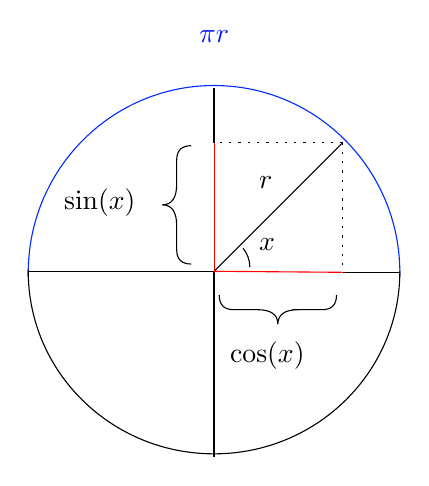
\begin{tikzpicture}[x=0.75pt,y=0.75pt,yscale=-1,xscale=1]
%uncomment if require: \path (0,300); %set diagram left start at 0, and has height of 300

%Straight Lines [id:da386434240814973] 
\draw    (67,163.5) -- (156.5,163.5) ;
%Straight Lines [id:da42068107268801314] 
\draw    (156.5,253) -- (156.5,163.5) ;
%Shape: Arc [id:dp3913962129512111] 
\draw  [draw opacity=0] (67,166.2) .. controls (66.99,165.57) and (66.98,164.94) .. (66.98,164.31) .. controls (66.98,114.43) and (107.06,74) .. (156.51,74) .. controls (205.95,74) and (246.03,114.43) .. (246.03,164.31) .. controls (246.03,164.87) and (246.02,165.43) .. (246.01,165.99) -- (156.51,164.31) -- cycle ; \draw  [color={rgb, 255:red, 0; green, 42; blue, 255 }  ,draw opacity=1 ] (67,166.2) .. controls (66.99,165.57) and (66.98,164.94) .. (66.98,164.31) .. controls (66.98,114.43) and (107.06,74) .. (156.51,74) .. controls (205.95,74) and (246.03,114.43) .. (246.03,164.31) .. controls (246.03,164.87) and (246.02,165.43) .. (246.01,165.99) ;
%Straight Lines [id:da11768574940811571] 
\draw [color={rgb, 255:red, 255; green, 0; blue, 0 }  ,draw opacity=1 ]   (156.5,163.5) -- (218.5,164) ;
%Shape: Arc [id:dp31810911811977405] 
\draw  [draw opacity=0] (246.01,163.2) .. controls (246.01,163.3) and (246.02,163.4) .. (246.02,163.5) .. controls (246.02,212.08) and (205.94,251.46) .. (156.5,251.46) .. controls (107.06,251.46) and (66.98,212.08) .. (66.98,163.5) .. controls (66.98,163.29) and (66.99,163.08) .. (66.99,162.88) -- (156.5,163.5) -- cycle ; \draw   (246.01,163.2) .. controls (246.01,163.3) and (246.02,163.4) .. (246.02,163.5) .. controls (246.02,212.08) and (205.94,251.46) .. (156.5,251.46) .. controls (107.06,251.46) and (66.98,212.08) .. (66.98,163.5) .. controls (66.98,163.29) and (66.99,163.08) .. (66.99,162.88) ;
%Straight Lines [id:da5653362033776077] 
\draw    (218.5,101.5) -- (156.5,163.5) ;
%Shape: Arc [id:dp6851417678817022] 
\draw  [draw opacity=0] (170.45,152.38) .. controls (172.51,154.85) and (173.75,158.03) .. (173.75,161.5) -- (159.5,161.5) -- cycle ; \draw   (170.45,152.38) .. controls (172.51,154.85) and (173.75,158.03) .. (173.75,161.5) ;
%Straight Lines [id:da6792923713073786] 
\draw [color={rgb, 255:red, 0; green, 0; blue, 0 }  ,draw opacity=1 ] [dash pattern={on 0.84pt off 2.51pt}]  (218.5,101.5) -- (218.5,164) ;
%Straight Lines [id:da7704392572078389] 
\draw    (218.5,164) -- (246.01,164) ;
%Straight Lines [id:da03395672094050417] 
\draw  [dash pattern={on 0.84pt off 2.51pt}]  (218.5,101.5) -- (156.5,101.5) ;
%Straight Lines [id:da2459100515519198] 
\draw [color={rgb, 255:red, 255; green, 0; blue, 0 }  ,draw opacity=1 ]   (156.51,101.5) -- (156.51,123) -- (156.51,164.31) ;
%Straight Lines [id:da08850824038464977] 
\draw    (156.5,101.5) -- (156.5,75) ;
%Shape: Brace [id:dp03532467075132828] 
\draw   (145.5,103) .. controls (140.83,103) and (138.5,105.33) .. (138.5,110) -- (138.5,121.5) .. controls (138.5,128.17) and (136.17,131.5) .. (131.5,131.5) .. controls (136.17,131.5) and (138.5,134.83) .. (138.5,141.5)(138.5,138.5) -- (138.5,153) .. controls (138.5,157.67) and (140.83,160) .. (145.5,160) ;
%Shape: Brace [id:dp6579804825737726] 
\draw   (159,175) .. controls (159,179.67) and (161.33,182) .. (166,182) -- (177.25,182) .. controls (183.92,182) and (187.25,184.33) .. (187.25,189) .. controls (187.25,184.33) and (190.58,182) .. (197.25,182)(194.25,182) -- (208.5,182) .. controls (213.17,182) and (215.5,179.67) .. (215.5,175) ;

% Text Node
\draw (177,146.4) node [anchor=north west][inner sep=0.75pt]    {$x$};
% Text Node
\draw (83,122.4) node [anchor=north west][inner sep=0.75pt]    {$\sin( x)$};
% Text Node
\draw (177,116.4) node [anchor=north west][inner sep=0.75pt]    {$r$};
% Text Node
\draw (163,196.4) node [anchor=north west][inner sep=0.75pt]    {$\cos( x)$};
% Text Node
\draw (148,46.4) node [anchor=north west][inner sep=0.75pt]  [color={rgb, 255:red, 0; green, 24; blue, 255 }  ,opacity=1 ]  {$\pi r$};


\end{tikzpicture}

They give us the answer as a ratio of or as a percentage of \( r \).

Because the domain of these functions is a partition of the reals,
they are periodic with a period of \( 2\pi \).
This means
\[ \cos(x) = \cos(x + 2\pi) \]
and
\[ \sin(x) = \sin(x + 2\pi). \]

We can specify the coordinates of a point in two ways.
First, we can specify it's position along each axis (rectangular form):
\[ (r \cos(x), r \sin(x)), \]
or we can just give the radius and angle (polar form):
\[ (r, x). \]

\newpage
The function \( \tan \) is just the ratio

\tikzset{every picture/.style={line width=0.75pt}} %set default line width to 0.75pt        

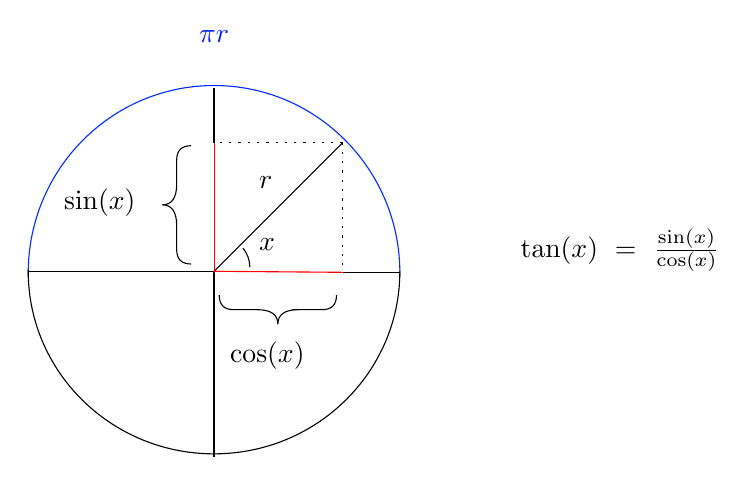
\begin{tikzpicture}[x=0.75pt,y=0.75pt,yscale=-1,xscale=1]
%uncomment if require: \path (0,300); %set diagram left start at 0, and has height of 300

%Straight Lines [id:da7835883213561495] 
\draw    (87,172.89) -- (176.5,172.89) ;
%Straight Lines [id:da2069592864789831] 
\draw    (176.5,262.39) -- (176.5,172.89) ;
%Shape: Arc [id:dp7505851293217748] 
\draw  [draw opacity=0] (87,175.59) .. controls (86.99,174.96) and (86.98,174.33) .. (86.98,173.69) .. controls (86.98,123.82) and (127.06,83.39) .. (176.51,83.39) .. controls (225.95,83.39) and (266.03,123.82) .. (266.03,173.69) .. controls (266.03,174.26) and (266.02,174.82) .. (266.01,175.38) -- (176.51,173.69) -- cycle ; \draw  [color={rgb, 255:red, 0; green, 42; blue, 255 }  ,draw opacity=1 ] (87,175.59) .. controls (86.99,174.96) and (86.98,174.33) .. (86.98,173.69) .. controls (86.98,123.82) and (127.06,83.39) .. (176.51,83.39) .. controls (225.95,83.39) and (266.03,123.82) .. (266.03,173.69) .. controls (266.03,174.26) and (266.02,174.82) .. (266.01,175.38) ;
%Straight Lines [id:da2175596906060845] 
\draw [color={rgb, 255:red, 255; green, 0; blue, 0 }  ,draw opacity=1 ]   (176.5,172.89) -- (238.5,173.39) ;
%Shape: Arc [id:dp9218401449375668] 
\draw  [draw opacity=0] (266.01,172.59) .. controls (266.01,172.69) and (266.02,172.79) .. (266.02,172.89) .. controls (266.02,221.47) and (225.94,260.85) .. (176.5,260.85) .. controls (127.06,260.85) and (86.98,221.47) .. (86.98,172.89) .. controls (86.98,172.68) and (86.99,172.47) .. (86.99,172.26) -- (176.5,172.89) -- cycle ; \draw   (266.01,172.59) .. controls (266.01,172.69) and (266.02,172.79) .. (266.02,172.89) .. controls (266.02,221.47) and (225.94,260.85) .. (176.5,260.85) .. controls (127.06,260.85) and (86.98,221.47) .. (86.98,172.89) .. controls (86.98,172.68) and (86.99,172.47) .. (86.99,172.26) ;
%Straight Lines [id:da791320368124574] 
\draw    (238.5,110.89) -- (176.5,172.89) ;
%Shape: Arc [id:dp7432023456736092] 
\draw  [draw opacity=0] (190.45,161.76) .. controls (192.51,164.24) and (193.75,167.42) .. (193.75,170.89) -- (179.5,170.89) -- cycle ; \draw   (190.45,161.76) .. controls (192.51,164.24) and (193.75,167.42) .. (193.75,170.89) ;
%Straight Lines [id:da5824483322026068] 
\draw [color={rgb, 255:red, 0; green, 0; blue, 0 }  ,draw opacity=1 ] [dash pattern={on 0.84pt off 2.51pt}]  (238.5,110.89) -- (238.5,173.39) ;
%Straight Lines [id:da47524866156438517] 
\draw    (238.5,173.39) -- (266.01,173.39) ;
%Straight Lines [id:da09780504576387938] 
\draw  [dash pattern={on 0.84pt off 2.51pt}]  (238.5,110.89) -- (176.5,110.89) ;
%Straight Lines [id:da3548368319368671] 
\draw [color={rgb, 255:red, 255; green, 0; blue, 0 }  ,draw opacity=1 ]   (176.51,110.89) -- (176.51,132.39) -- (176.51,173.69) ;
%Straight Lines [id:da8124693094798018] 
\draw    (176.5,110.89) -- (176.5,84.39) ;
%Shape: Brace [id:dp5137034581949013] 
\draw   (165.5,112.39) .. controls (160.83,112.39) and (158.5,114.72) .. (158.5,119.39) -- (158.5,130.89) .. controls (158.5,137.56) and (156.17,140.89) .. (151.5,140.89) .. controls (156.17,140.89) and (158.5,144.22) .. (158.5,150.89)(158.5,147.89) -- (158.5,162.39) .. controls (158.5,167.06) and (160.83,169.39) .. (165.5,169.39) ;
%Shape: Brace [id:dp12726316775693558] 
\draw   (179,184.39) .. controls (179,189.06) and (181.33,191.39) .. (186,191.39) -- (197.25,191.39) .. controls (203.92,191.39) and (207.25,193.72) .. (207.25,198.39) .. controls (207.25,193.72) and (210.58,191.39) .. (217.25,191.39)(214.25,191.39) -- (228.5,191.39) .. controls (233.17,191.39) and (235.5,189.06) .. (235.5,184.39) ;

% Text Node
\draw (197,155.79) node [anchor=north west][inner sep=0.75pt]    {$x$};
% Text Node
\draw (103,131.79) node [anchor=north west][inner sep=0.75pt]    {$\sin( x)$};
% Text Node
\draw (197,125.79) node [anchor=north west][inner sep=0.75pt]    {$r$};
% Text Node
\draw (183,205.79) node [anchor=north west][inner sep=0.75pt]    {$\cos( x)$};
% Text Node
\draw (168,55.79) node [anchor=north west][inner sep=0.75pt]  [color={rgb, 255:red, 0; green, 24; blue, 255 }  ,opacity=1 ]  {$\pi r$};
% Text Node
\draw (323,151.4) node [anchor=north west][inner sep=0.75pt]    {$\tan( x) \ =\ \frac{\sin( x)}{\cos( x)}$};


\end{tikzpicture}

We can think of this as the slope of the line through the point at the angle.


\newpage
\section{Complex Numbers}

The complex numbers are a number system or a field just like the reals.
Each complex number is made of two parts: the real part and the imaginary part.
We can represent these on a plane with one axis being real and the other being imaginary.
Take a complex number \( z = a + bi \).

\tikzset{every picture/.style={line width=0.75pt}} %set default line width to 0.75pt        

\tikzset{every picture/.style={line width=0.75pt}} %set default line width to 0.75pt        

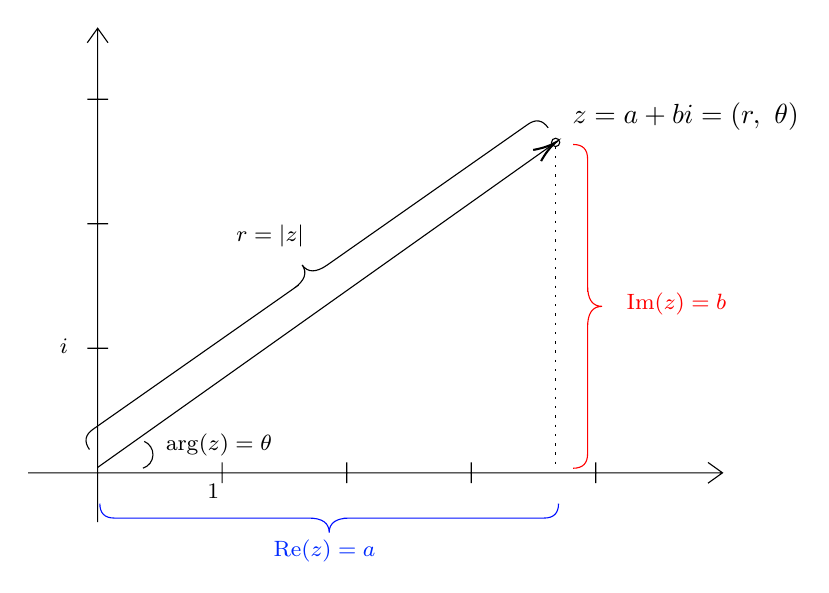
\begin{tikzpicture}[x=0.75pt,y=0.75pt,yscale=-1,xscale=1]
%uncomment if require: \path (0,300); %set diagram left start at 0, and has height of 300

%Shape: Axis 2D [id:dp4700217616893223] 
\draw  (46,246.2) -- (380.5,246.2)(79.45,32) -- (79.45,270) (373.5,241.2) -- (380.5,246.2) -- (373.5,251.2) (74.45,39) -- (79.45,32) -- (84.45,39) (139.45,241.2) -- (139.45,251.2)(199.45,241.2) -- (199.45,251.2)(259.45,241.2) -- (259.45,251.2)(319.45,241.2) -- (319.45,251.2)(74.45,186.2) -- (84.45,186.2)(74.45,126.2) -- (84.45,126.2)(74.45,66.2) -- (84.45,66.2) ;
\draw   ;
%Straight Lines [id:da1141401634967012] 
\draw    (79.45,243.6) -- (298.47,88.16) ;
\draw [shift={(300.1,87)}, rotate = 504.64] [color={rgb, 255:red, 0; green, 0; blue, 0 }  ][line width=0.75]    (10.93,-3.29) .. controls (6.95,-1.4) and (3.31,-0.3) .. (0,0) .. controls (3.31,0.3) and (6.95,1.4) .. (10.93,3.29)   ;
%Shape: Circle [id:dp44110533792950923] 
\draw   (298.1,87) .. controls (298.1,85.9) and (299,85) .. (300.1,85) .. controls (301.2,85) and (302.1,85.9) .. (302.1,87) .. controls (302.1,88.1) and (301.2,89) .. (300.1,89) .. controls (299,89) and (298.1,88.1) .. (298.1,87) -- cycle ;
%Shape: Arc [id:dp03726885849887451] 
\draw  [draw opacity=0] (101.9,231.06) .. controls (104.44,232.14) and (106.18,234.69) .. (106.1,237.61) .. controls (106.01,240.63) and (103.98,243.14) .. (101.25,243.99) -- (99.21,237.4) -- cycle ; \draw   (101.9,231.06) .. controls (104.44,232.14) and (106.18,234.69) .. (106.1,237.61) .. controls (106.01,240.63) and (103.98,243.14) .. (101.25,243.99) ;
%Shape: Brace [id:dp38892828645713595] 
\draw   (296.5,80) .. controls (293.82,76.18) and (290.57,75.61) .. (286.75,78.29) -- (190.16,146.02) .. controls (184.71,149.85) and (180.64,149.85) .. (177.96,146.03) .. controls (180.64,149.85) and (179.25,153.67) .. (173.79,157.5)(176.24,155.78) -- (77.2,225.23) .. controls (73.38,227.91) and (72.81,231.16) .. (75.49,234.98) ;
%Shape: Brace [id:dp00822474139118512] 
\draw  [color={rgb, 255:red, 0; green, 15; blue, 255 }  ,draw opacity=1 ] (80.5,261) .. controls (80.5,265.67) and (82.83,268) .. (87.5,268) -- (181,268) .. controls (187.67,268) and (191,270.33) .. (191,275) .. controls (191,270.33) and (194.33,268) .. (201,268)(198,268) -- (294.5,268) .. controls (299.17,268) and (301.5,265.67) .. (301.5,261) ;
%Shape: Brace [id:dp4128906105867539] 
\draw  [color={rgb, 255:red, 255; green, 0; blue, 0 }  ,draw opacity=1 ] (308.5,244) .. controls (313.17,244) and (315.5,241.67) .. (315.5,237) -- (315.5,176) .. controls (315.5,169.33) and (317.83,166) .. (322.5,166) .. controls (317.83,166) and (315.5,162.67) .. (315.5,156)(315.5,159) -- (315.5,95) .. controls (315.5,90.33) and (313.17,88) .. (308.5,88) ;
%Straight Lines [id:da26429163876661155] 
\draw  [dash pattern={on 0.84pt off 2.51pt}]  (300.1,89) -- (300.1,245) ;

% Text Node
\draw (60,180.4) node [anchor=north west][inner sep=0.75pt]  [font=\footnotesize]  {$i$};
% Text Node
\draw (131,250.4) node [anchor=north west][inner sep=0.75pt]  [font=\footnotesize]  {$1$};
% Text Node
\draw (111,226.4) node [anchor=north west][inner sep=0.75pt]  [font=\footnotesize]  {$\arg( z) =\theta $};
% Text Node
\draw (333,158.4) node [anchor=north west][inner sep=0.75pt]  [font=\footnotesize,color={rgb, 255:red, 255; green, 0; blue, 0 }  ,opacity=1 ]  {$\Im ( z) =b$};
% Text Node
\draw (163,277.4) node [anchor=north west][inner sep=0.75pt]  [font=\footnotesize,color={rgb, 255:red, 0; green, 42; blue, 255 }  ,opacity=1 ]  {$\Re ( z) =a$};
% Text Node
\draw (145,125.4) node [anchor=north west][inner sep=0.75pt]  [font=\footnotesize]  {$r=|z|$};
% Text Node
\draw (307,66.4) node [anchor=north west][inner sep=0.75pt]    {$z=a+bi=( r,\ \theta )$};


\end{tikzpicture}

From trigonometry, we know we can get the ratio of each part to the modulus,
or that \( a = r \cos(\theta) \)
and \( b = r \sin(\theta) \).
The we can represent \( z \) as
\[ z = r(\cos(\theta) + i \sin(\theta)). \]

\subsection{Operations}

We define complex addition as vector addition,
which means component wise addition.
So \[ (a_1 + b_1 i) + (a_2 + b_2 i) = (a_1 + b_1 + (a_2 + b_2)i). \]
This is also a translation.

\tikzset{every picture/.style={line width=0.75pt}} %set default line width to 0.75pt        

\noindent
\begin{tikzpicture}[x=0.75pt,y=0.75pt,yscale=-1,xscale=1]
%uncomment if require: \path (0,300); %set diagram left start at 0, and has height of 300

%Shape: Axis 2D [id:dp9274384698564448] 
\draw  (50,160) -- (515.5,160)(163.5,40) -- (163.5,262) (508.5,155) -- (515.5,160) -- (508.5,165) (158.5,47) -- (163.5,40) -- (168.5,47) (196.5,155) -- (196.5,165)(229.5,155) -- (229.5,165)(262.5,155) -- (262.5,165)(295.5,155) -- (295.5,165)(328.5,155) -- (328.5,165)(361.5,155) -- (361.5,165)(394.5,155) -- (394.5,165)(427.5,155) -- (427.5,165)(460.5,155) -- (460.5,165)(493.5,155) -- (493.5,165)(130.5,155) -- (130.5,165)(97.5,155) -- (97.5,165)(64.5,155) -- (64.5,165)(158.5,127) -- (168.5,127)(158.5,94) -- (168.5,94)(158.5,61) -- (168.5,61)(158.5,193) -- (168.5,193)(158.5,226) -- (168.5,226) ;
\draw   ;
%Straight Lines [id:da0662747562558057] 
\draw    (163.5,160) -- (256.05,72.38) ;
\draw [shift={(257.5,71)}, rotate = 496.57] [color={rgb, 255:red, 0; green, 0; blue, 0 }  ][line width=0.75]    (10.93,-3.29) .. controls (6.95,-1.4) and (3.31,-0.3) .. (0,0) .. controls (3.31,0.3) and (6.95,1.4) .. (10.93,3.29)   ;
%Straight Lines [id:da2938560981570685] 
\draw    (163.5,160) -- (253.67,199.2) ;
\draw [shift={(255.5,200)}, rotate = 203.5] [color={rgb, 255:red, 0; green, 0; blue, 0 }  ][line width=0.75]    (10.93,-3.29) .. controls (6.95,-1.4) and (3.31,-0.3) .. (0,0) .. controls (3.31,0.3) and (6.95,1.4) .. (10.93,3.29)   ;
%Straight Lines [id:da49802555821043903] 
\draw  [dash pattern={on 0.84pt off 2.51pt}]  (257.5,71) -- (347.67,110.2) ;
\draw [shift={(349.5,111)}, rotate = 203.5] [color={rgb, 255:red, 0; green, 0; blue, 0 }  ][line width=0.75]    (10.93,-3.29) .. controls (6.95,-1.4) and (3.31,-0.3) .. (0,0) .. controls (3.31,0.3) and (6.95,1.4) .. (10.93,3.29)   ;
%Straight Lines [id:da9013882168552714] 
\draw [color={rgb, 255:red, 255; green, 0; blue, 0 }  ,draw opacity=1 ]   (163.5,160) -- (347.57,111.51) ;
\draw [shift={(349.5,111)}, rotate = 525.24] [color={rgb, 255:red, 255; green, 0; blue, 0 }  ,draw opacity=1 ][line width=0.75]    (10.93,-3.29) .. controls (6.95,-1.4) and (3.31,-0.3) .. (0,0) .. controls (3.31,0.3) and (6.95,1.4) .. (10.93,3.29)   ;

% Text Node
\draw (216,71.4) node [anchor=north west][inner sep=0.75pt]    {$z_{1}$};
% Text Node
\draw (254,208.4) node [anchor=north west][inner sep=0.75pt]    {$z_{2}$};
% Text Node
\draw (357,99.4) node [anchor=north west][inner sep=0.75pt]  [color={rgb, 255:red, 255; green, 0; blue, 0 }  ,opacity=1 ]  {$z_{1} \ +z_{2}$};


\end{tikzpicture}

We define complex multiplication as multiplying the moduluses and adding the angles.
So \( (r, \theta)(p, \phi) = (rp, \theta + \phi) \).
This is also a rotation and a scaling (dilation).

\tikzset{every picture/.style={line width=0.75pt}} %set default line width to 0.75pt        

\noindent
\begin{tikzpicture}[x=0.75pt,y=0.75pt,yscale=-1,xscale=1]
%uncomment if require: \path (0,300); %set diagram left start at 0, and has height of 300

%Shape: Axis 2D [id:dp049849838656989] 
\draw  (70,180) -- (535.5,180)(183.5,60) -- (183.5,282) (528.5,175) -- (535.5,180) -- (528.5,185) (178.5,67) -- (183.5,60) -- (188.5,67) (216.5,175) -- (216.5,185)(249.5,175) -- (249.5,185)(282.5,175) -- (282.5,185)(315.5,175) -- (315.5,185)(348.5,175) -- (348.5,185)(381.5,175) -- (381.5,185)(414.5,175) -- (414.5,185)(447.5,175) -- (447.5,185)(480.5,175) -- (480.5,185)(513.5,175) -- (513.5,185)(150.5,175) -- (150.5,185)(117.5,175) -- (117.5,185)(84.5,175) -- (84.5,185)(178.5,147) -- (188.5,147)(178.5,114) -- (188.5,114)(178.5,81) -- (188.5,81)(178.5,213) -- (188.5,213)(178.5,246) -- (188.5,246) ;
\draw   ;
%Straight Lines [id:da9974234043672462] 
\draw    (183.5,180) -- (276.05,92.38) ;
\draw [shift={(277.5,91)}, rotate = 496.57] [color={rgb, 255:red, 0; green, 0; blue, 0 }  ][line width=0.75]    (10.93,-3.29) .. controls (6.95,-1.4) and (3.31,-0.3) .. (0,0) .. controls (3.31,0.3) and (6.95,1.4) .. (10.93,3.29)   ;
%Straight Lines [id:da20657379122009134] 
\draw    (183.5,180) -- (273.67,219.2) ;
\draw [shift={(275.5,220)}, rotate = 203.5] [color={rgb, 255:red, 0; green, 0; blue, 0 }  ][line width=0.75]    (10.93,-3.29) .. controls (6.95,-1.4) and (3.31,-0.3) .. (0,0) .. controls (3.31,0.3) and (6.95,1.4) .. (10.93,3.29)   ;
%Shape: Arc [id:dp5803037905068104] 
\draw  [draw opacity=0] (200.9,165.06) .. controls (203.44,166.14) and (205.18,168.69) .. (205.1,171.61) .. controls (205.01,174.63) and (202.98,177.14) .. (200.25,177.99) -- (198.21,171.4) -- cycle ; \draw   (200.9,165.06) .. controls (203.44,166.14) and (205.18,168.69) .. (205.1,171.61) .. controls (205.01,174.63) and (202.98,177.14) .. (200.25,177.99) ;
%Shape: Arc [id:dp7047653051043884] 
\draw  [draw opacity=0] (207.18,181.49) .. controls (209,182.26) and (210.25,184.09) .. (210.19,186.18) .. controls (210.12,188.34) and (208.68,190.13) .. (206.72,190.74) -- (205.26,186.03) -- cycle ; \draw   (207.18,181.49) .. controls (209,182.26) and (210.25,184.09) .. (210.19,186.18) .. controls (210.12,188.34) and (208.68,190.13) .. (206.72,190.74) ;
%Straight Lines [id:da4324446373354387] 
\draw [color={rgb, 255:red, 255; green, 0; blue, 0 }  ,draw opacity=1 ]   (183.5,180) -- (513.56,97.49) ;
\draw [shift={(515.5,97)}, rotate = 525.96] [color={rgb, 255:red, 255; green, 0; blue, 0 }  ,draw opacity=1 ][line width=0.75]    (10.93,-3.29) .. controls (6.95,-1.4) and (3.31,-0.3) .. (0,0) .. controls (3.31,0.3) and (6.95,1.4) .. (10.93,3.29)   ;
%Shape: Arc [id:dp5325215380673752] 
\draw  [draw opacity=0] (235.18,168.49) .. controls (237,169.26) and (238.25,171.09) .. (238.19,173.18) .. controls (238.12,175.34) and (236.68,177.13) .. (234.72,177.74) -- (233.26,173.03) -- cycle ; \draw  [color={rgb, 255:red, 255; green, 0; blue, 0 }  ,draw opacity=1 ] (235.18,168.49) .. controls (237,169.26) and (238.25,171.09) .. (238.19,173.18) .. controls (238.12,175.34) and (236.68,177.13) .. (234.72,177.74) ;

% Text Node
\draw (250,72.4) node [anchor=north west][inner sep=0.75pt]    {$z_{1}$};
% Text Node
\draw (274,228.4) node [anchor=north west][inner sep=0.75pt]    {$z_{2}$};
% Text Node
\draw (208,154.4) node [anchor=north west][inner sep=0.75pt]  [font=\footnotesize]  {$\theta $};
% Text Node
\draw (221,180.4) node [anchor=north west][inner sep=0.75pt]  [font=\footnotesize]  {$\phi $};
% Text Node
\draw (211,125.4) node [anchor=north west][inner sep=0.75pt]    {$r$};
% Text Node
\draw (221,208.4) node [anchor=north west][inner sep=0.75pt]    {$p$};
% Text Node
\draw (370,105.4) node [anchor=north west][inner sep=0.75pt]  [color={rgb, 255:red, 255; green, 0; blue, 0 }  ,opacity=1 ]  {$rp$};
% Text Node
\draw (525,84.4) node [anchor=north west][inner sep=0.75pt]  [color={rgb, 255:red, 255; green, 0; blue, 0 }  ,opacity=1 ]  {$z_{1} z_{2}$};
% Text Node
\draw (265,161.4) node [anchor=north west][inner sep=0.75pt]  [font=\footnotesize,color={rgb, 255:red, 255; green, 0; blue, 0 }  ,opacity=1 ]  {$\theta +\phi $};


\end{tikzpicture}

This is a rotation and a scaling (dilation).

Algebraically, multiplication is
\[ (a + bi)(c + di) = (ac - bd) + i (ad + bc). \]
This is because multiplication and addition are distributive.



\subsection{Euler's Formula}

We know complex multiplication is just rotating a vector.
We can also define complex exponentiation.
Take a unit circle.
Define \( e^{i} \) to be a rotation of 1 radian around the circle.

\tikzset{every picture/.style={line width=0.75pt}} %set default line width to 0.75pt        

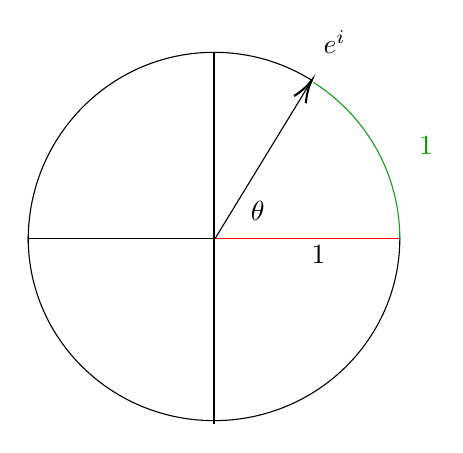
\begin{tikzpicture}[x=0.75pt,y=0.75pt,yscale=-1,xscale=1]
%uncomment if require: \path (0,300); %set diagram left start at 0, and has height of 300

%Straight Lines [id:da9612116411157848] 
\draw    (80,144.5) -- (169.5,144.5) ;
%Straight Lines [id:da20874309323783247] 
\draw    (169.5,234) -- (169.5,55) ;
%Shape: Arc [id:dp92425960700565] 
\draw  [draw opacity=0] (80,147.2) .. controls (79.99,146.57) and (79.98,145.94) .. (79.98,145.31) .. controls (79.98,95.43) and (120.06,55) .. (169.51,55) .. controls (186.78,55) and (202.91,59.94) .. (216.58,68.48) -- (169.51,145.31) -- cycle ; \draw  [color={rgb, 255:red, 0; green, 0; blue, 0 }  ,draw opacity=1 ] (80,147.2) .. controls (79.99,146.57) and (79.98,145.94) .. (79.98,145.31) .. controls (79.98,95.43) and (120.06,55) .. (169.51,55) .. controls (186.78,55) and (202.91,59.94) .. (216.58,68.48) ;
%Straight Lines [id:da7022096021136846] 
\draw [color={rgb, 255:red, 255; green, 0; blue, 0 }  ,draw opacity=1 ]   (169.5,144.5) -- (259.02,144.5) ;
%Shape: Arc [id:dp30235297301165553] 
\draw  [draw opacity=0] (259.01,144.2) .. controls (259.01,144.3) and (259.02,144.4) .. (259.02,144.5) .. controls (259.02,193.08) and (218.94,232.46) .. (169.5,232.46) .. controls (120.06,232.46) and (79.98,193.08) .. (79.98,144.5) .. controls (79.98,144.29) and (79.99,144.08) .. (79.99,143.88) -- (169.5,144.5) -- cycle ; \draw   (259.01,144.2) .. controls (259.01,144.3) and (259.02,144.4) .. (259.02,144.5) .. controls (259.02,193.08) and (218.94,232.46) .. (169.5,232.46) .. controls (120.06,232.46) and (79.98,193.08) .. (79.98,144.5) .. controls (79.98,144.29) and (79.99,144.08) .. (79.99,143.88) ;
%Shape: Arc [id:dp5841795559043887] 
\draw  [draw opacity=0] (217.43,69.53) .. controls (242.45,85.33) and (259.04,113.23) .. (259.01,144.98) -- (169.91,144.9) -- cycle ; \draw  [color={rgb, 255:red, 22; green, 156; blue, 30 }  ,draw opacity=1 ] (217.43,69.53) .. controls (242.45,85.33) and (259.04,113.23) .. (259.01,144.98) ;
%Straight Lines [id:da14699259993103542] 
\draw    (169.91,144.9) -- (215.54,70.19) ;
\draw [shift={(216.58,68.48)}, rotate = 481.41] [color={rgb, 255:red, 0; green, 0; blue, 0 }  ][line width=0.75]    (10.93,-3.29) .. controls (6.95,-1.4) and (3.31,-0.3) .. (0,0) .. controls (3.31,0.3) and (6.95,1.4) .. (10.93,3.29)   ;

% Text Node
\draw (215.25,146.9) node [anchor=north west][inner sep=0.75pt]    {$1$};
% Text Node
\draw (267,94.4) node [anchor=north west][inner sep=0.75pt]  [color={rgb, 255:red, 12; green, 148; blue, 0 }  ,opacity=1 ]  {$1$};
% Text Node
\draw (221,43.4) node [anchor=north west][inner sep=0.75pt]    {$e^{i}$};
% Text Node
\draw (186,125.4) node [anchor=north west][inner sep=0.75pt]    {$\theta $};


\end{tikzpicture}


We can represent this rotation as the complex number
\( (1, \theta) = \cos(\theta) + i\sin(\theta) \).
Then the function \( e^{ix} \) just represents a rotation at a rate of
\( e^i \) radians per \( x \).
Exponentiation of another base is just a change of rates.
For example, \( 2^i = e^{i \ln(2)} \).

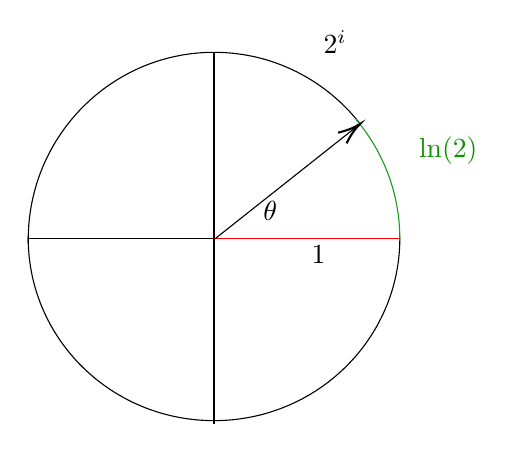
\begin{tikzpicture}[x=0.75pt,y=0.75pt,yscale=-1,xscale=1]
%uncomment if require: \path (0,300); %set diagram left start at 0, and has height of 300

%Straight Lines [id:da5300201460555855] 
\draw    (100,164.5) -- (189.5,164.5) ;
%Straight Lines [id:da7209499549539827] 
\draw    (189.5,254) -- (189.5,75) ;
%Shape: Arc [id:dp1477018513826992] 
\draw  [draw opacity=0] (100,167.2) .. controls (99.99,166.57) and (99.98,165.94) .. (99.98,165.31) .. controls (99.98,115.43) and (140.06,75) .. (189.51,75) .. controls (218.06,75) and (243.49,88.49) .. (259.88,109.49) -- (189.51,165.31) -- cycle ; \draw  [color={rgb, 255:red, 0; green, 0; blue, 0 }  ,draw opacity=1 ] (100,167.2) .. controls (99.99,166.57) and (99.98,165.94) .. (99.98,165.31) .. controls (99.98,115.43) and (140.06,75) .. (189.51,75) .. controls (218.06,75) and (243.49,88.49) .. (259.88,109.49) ;
%Straight Lines [id:da8647831039135583] 
\draw [color={rgb, 255:red, 255; green, 0; blue, 0 }  ,draw opacity=1 ]   (189.5,164.5) -- (279.02,164.5) ;
%Shape: Arc [id:dp5268217987140125] 
\draw  [draw opacity=0] (279.01,164.2) .. controls (279.01,164.3) and (279.02,164.4) .. (279.02,164.5) .. controls (279.02,213.08) and (238.94,252.46) .. (189.5,252.46) .. controls (140.06,252.46) and (99.98,213.08) .. (99.98,164.5) .. controls (99.98,164.29) and (99.99,164.08) .. (99.99,163.88) -- (189.5,164.5) -- cycle ; \draw   (279.01,164.2) .. controls (279.01,164.3) and (279.02,164.4) .. (279.02,164.5) .. controls (279.02,213.08) and (238.94,252.46) .. (189.5,252.46) .. controls (140.06,252.46) and (99.98,213.08) .. (99.98,164.5) .. controls (99.98,164.29) and (99.99,164.08) .. (99.99,163.88) ;
%Shape: Arc [id:dp1302089202448049] 
\draw  [draw opacity=0] (257.91,107.34) .. controls (271.09,122.89) and (279.03,143.02) .. (279.01,164.98) -- (189.91,164.9) -- cycle ; \draw  [color={rgb, 255:red, 22; green, 156; blue, 30 }  ,draw opacity=1 ] (257.91,107.34) .. controls (271.09,122.89) and (279.03,143.02) .. (279.01,164.98) ;
%Straight Lines [id:da04674799293912846] 
\draw    (189.91,164.9) -- (258.31,110.73) ;
\draw [shift={(259.88,109.49)}, rotate = 501.62] [color={rgb, 255:red, 0; green, 0; blue, 0 }  ][line width=0.75]    (10.93,-3.29) .. controls (6.95,-1.4) and (3.31,-0.3) .. (0,0) .. controls (3.31,0.3) and (6.95,1.4) .. (10.93,3.29)   ;

% Text Node
\draw (235.25,166.9) node [anchor=north west][inner sep=0.75pt]    {$1$};
% Text Node
\draw (287,114.4) node [anchor=north west][inner sep=0.75pt]  [color={rgb, 255:red, 12; green, 148; blue, 0 }  ,opacity=1 ]  {$\ln( 2)$};
% Text Node
\draw (241,63.4) node [anchor=north west][inner sep=0.75pt]    {$2^{i}$};
% Text Node
\draw (212,145.4) node [anchor=north west][inner sep=0.75pt]    {$\theta $};


\end{tikzpicture}

Note that we can represent any complex number in exponential form.
For example, \( (r, \theta) = re^{i \theta} \).

\begin{tikzpicture}[x=0.75pt,y=0.75pt,yscale=-1,xscale=1]
%uncomment if require: \path (0,300); %set diagram left start at 0, and has height of 300

%Straight Lines [id:da9237016542405356] 
\draw    (100,164.5) -- (189.5,164.5) ;
%Straight Lines [id:da40547936095337156] 
\draw    (189.5,254) -- (189.5,75) ;
%Shape: Arc [id:dp7128392210866575] 
\draw  [draw opacity=0] (100,167.2) .. controls (99.99,166.57) and (99.98,165.94) .. (99.98,165.31) .. controls (99.98,143.29) and (107.79,123.12) .. (120.77,107.45) -- (189.51,165.31) -- cycle ; \draw  [color={rgb, 255:red, 0; green, 0; blue, 0 }  ,draw opacity=1 ] (100,167.2) .. controls (99.99,166.57) and (99.98,165.94) .. (99.98,165.31) .. controls (99.98,143.29) and (107.79,123.12) .. (120.77,107.45) ;
%Straight Lines [id:da21620653870476014] 
\draw [color={rgb, 255:red, 255; green, 0; blue, 0 }  ,draw opacity=1 ]   (189.5,164.5) -- (279.02,164.5) ;
%Shape: Arc [id:dp7588297786268827] 
\draw  [draw opacity=0] (279.01,164.2) .. controls (279.01,164.3) and (279.02,164.4) .. (279.02,164.5) .. controls (279.02,213.08) and (238.94,252.46) .. (189.5,252.46) .. controls (140.06,252.46) and (99.98,213.08) .. (99.98,164.5) .. controls (99.98,164.29) and (99.99,164.08) .. (99.99,163.88) -- (189.5,164.5) -- cycle ; \draw   (279.01,164.2) .. controls (279.01,164.3) and (279.02,164.4) .. (279.02,164.5) .. controls (279.02,213.08) and (238.94,252.46) .. (189.5,252.46) .. controls (140.06,252.46) and (99.98,213.08) .. (99.98,164.5) .. controls (99.98,164.29) and (99.99,164.08) .. (99.99,163.88) ;
%Shape: Arc [id:dp6903926186187812] 
\draw  [draw opacity=0] (121.78,107.49) .. controls (138.2,88.03) and (162.8,75.7) .. (190.25,75.81) .. controls (239.37,76) and (279.05,115.9) .. (279.01,164.98) -- (189.91,164.9) -- cycle ; \draw  [color={rgb, 255:red, 22; green, 156; blue, 30 }  ,draw opacity=1 ] (121.78,107.49) .. controls (138.2,88.03) and (162.8,75.7) .. (190.25,75.81) .. controls (239.37,76) and (279.05,115.9) .. (279.01,164.98) ;
%Straight Lines [id:da5011183866413846] 
\draw    (189.91,164.9) -- (43.05,45.26) ;
\draw [shift={(41.5,44)}, rotate = 399.16999999999996] [color={rgb, 255:red, 0; green, 0; blue, 0 }  ][line width=0.75]    (10.93,-3.29) .. controls (6.95,-1.4) and (3.31,-0.3) .. (0,0) .. controls (3.31,0.3) and (6.95,1.4) .. (10.93,3.29)   ;

% Text Node
\draw (235.25,166.9) node [anchor=north west][inner sep=0.75pt]    {$1$};
% Text Node
\draw (271,103.4) node [anchor=north west][inner sep=0.75pt]  [color={rgb, 255:red, 12; green, 148; blue, 0 }  ,opacity=1 ]  {$\theta $};
% Text Node
\draw (60,27.4) node [anchor=north west][inner sep=0.75pt]    {$re^{i\theta }$};
% Text Node
\draw (191,140.4) node [anchor=north west][inner sep=0.75pt]    {$\theta $};


\end{tikzpicture}


\section{Identities}

We have \( \Re(z) = \frac{1}{2} (z + \bar z) \)
or \( \cos(x) = \frac{e^{ix} + e^{-ix}}{2} \).

\begin{tikzpicture}[x=0.75pt,y=0.75pt,yscale=-1,xscale=1]
%uncomment if require: \path (0,300); %set diagram left start at 0, and has height of 300

%Shape: Axis 2D [id:dp8866960351689678] 
\draw  (70,180) -- (535.5,180)(183.5,60) -- (183.5,282) (528.5,175) -- (535.5,180) -- (528.5,185) (178.5,67) -- (183.5,60) -- (188.5,67) (216.5,175) -- (216.5,185)(249.5,175) -- (249.5,185)(282.5,175) -- (282.5,185)(315.5,175) -- (315.5,185)(348.5,175) -- (348.5,185)(381.5,175) -- (381.5,185)(414.5,175) -- (414.5,185)(447.5,175) -- (447.5,185)(480.5,175) -- (480.5,185)(513.5,175) -- (513.5,185)(150.5,175) -- (150.5,185)(117.5,175) -- (117.5,185)(84.5,175) -- (84.5,185)(178.5,147) -- (188.5,147)(178.5,114) -- (188.5,114)(178.5,81) -- (188.5,81)(178.5,213) -- (188.5,213)(178.5,246) -- (188.5,246) ;
\draw   ;
%Straight Lines [id:da6383715248173603] 
\draw    (183.5,180) -- (276.05,92.38) ;
\draw [shift={(277.5,91)}, rotate = 496.57] [color={rgb, 255:red, 0; green, 0; blue, 0 }  ][line width=0.75]    (10.93,-3.29) .. controls (6.95,-1.4) and (3.31,-0.3) .. (0,0) .. controls (3.31,0.3) and (6.95,1.4) .. (10.93,3.29)   ;
%Straight Lines [id:da29895452332777517] 
\draw    (183.5,180) -- (277.02,264.66) ;
\draw [shift={(278.5,266)}, rotate = 222.15] [color={rgb, 255:red, 0; green, 0; blue, 0 }  ][line width=0.75]    (10.93,-3.29) .. controls (6.95,-1.4) and (3.31,-0.3) .. (0,0) .. controls (3.31,0.3) and (6.95,1.4) .. (10.93,3.29)   ;
%Straight Lines [id:da5365051594905169] 
\draw  [dash pattern={on 0.84pt off 2.51pt}]  (277.5,91) -- (377.01,179.67) ;
\draw [shift={(378.5,181)}, rotate = 221.7] [color={rgb, 255:red, 0; green, 0; blue, 0 }  ][line width=0.75]    (10.93,-3.29) .. controls (6.95,-1.4) and (3.31,-0.3) .. (0,0) .. controls (3.31,0.3) and (6.95,1.4) .. (10.93,3.29)   ;
%Straight Lines [id:da13561474934708184] 
\draw [color={rgb, 255:red, 255; green, 0; blue, 0 }  ,draw opacity=1 ]   (183.5,180) -- (376.5,180.99) ;
\draw [shift={(378.5,181)}, rotate = 180.29] [color={rgb, 255:red, 255; green, 0; blue, 0 }  ,draw opacity=1 ][line width=0.75]    (10.93,-3.29) .. controls (6.95,-1.4) and (3.31,-0.3) .. (0,0) .. controls (3.31,0.3) and (6.95,1.4) .. (10.93,3.29)   ;
%Straight Lines [id:da9741647889679523] 
\draw  [dash pattern={on 0.84pt off 2.51pt}]  (277.5,91) -- (277.5,179) ;

% Text Node
\draw (270,68.4) node [anchor=north west][inner sep=0.75pt]    {$z$};
% Text Node
\draw (288,254.4) node [anchor=north west][inner sep=0.75pt]    {$\overline{z}$};
% Text Node
\draw (384,157.4) node [anchor=north west][inner sep=0.75pt]  [color={rgb, 255:red, 255; green, 0; blue, 0 }  ,opacity=1 ]  {$z+\overline{z}$};


\end{tikzpicture}

We have \( \Im(z) = \frac{1}{2}(z - \bar z) \)
or \( \sin(x) = \frac{e^{ix} - e^{-ix}}{2} \).

\begin{tikzpicture}[x=0.75pt,y=0.75pt,yscale=-1,xscale=1]
%uncomment if require: \path (0,300); %set diagram left start at 0, and has height of 300

%Shape: Axis 2D [id:dp6798239346637576] 
\draw  (82,202) -- (410.5,202)(140.5,8) -- (140.5,289) (403.5,197) -- (410.5,202) -- (403.5,207) (135.5,15) -- (140.5,8) -- (145.5,15) (173.5,197) -- (173.5,207)(206.5,197) -- (206.5,207)(239.5,197) -- (239.5,207)(272.5,197) -- (272.5,207)(305.5,197) -- (305.5,207)(338.5,197) -- (338.5,207)(371.5,197) -- (371.5,207)(107.5,197) -- (107.5,207)(135.5,169) -- (145.5,169)(135.5,136) -- (145.5,136)(135.5,103) -- (145.5,103)(135.5,70) -- (145.5,70)(135.5,37) -- (145.5,37)(135.5,235) -- (145.5,235)(135.5,268) -- (145.5,268) ;
\draw   ;
%Straight Lines [id:da44340582239633897] 
\draw    (139.5,200) -- (232.05,112.38) ;
\draw [shift={(233.5,111)}, rotate = 496.57] [color={rgb, 255:red, 0; green, 0; blue, 0 }  ][line width=0.75]    (10.93,-3.29) .. controls (6.95,-1.4) and (3.31,-0.3) .. (0,0) .. controls (3.31,0.3) and (6.95,1.4) .. (10.93,3.29)   ;
%Straight Lines [id:da7772236250141363] 
\draw  [dash pattern={on 0.84pt off 2.51pt}]  (233.5,111) -- (233.5,199) ;
%Straight Lines [id:da34998403337055295] 
\draw  [dash pattern={on 0.84pt off 2.51pt}]  (233.5,111) -- (142.95,25.37) ;
\draw [shift={(141.5,24)}, rotate = 403.4] [color={rgb, 255:red, 0; green, 0; blue, 0 }  ][line width=0.75]    (10.93,-3.29) .. controls (6.95,-1.4) and (3.31,-0.3) .. (0,0) .. controls (3.31,0.3) and (6.95,1.4) .. (10.93,3.29)   ;
%Straight Lines [id:da8180538641236395] 
\draw    (139.5,200) -- (233.02,284.66) ;
\draw [shift={(234.5,286)}, rotate = 222.15] [color={rgb, 255:red, 0; green, 0; blue, 0 }  ][line width=0.75]    (10.93,-3.29) .. controls (6.95,-1.4) and (3.31,-0.3) .. (0,0) .. controls (3.31,0.3) and (6.95,1.4) .. (10.93,3.29)   ;
%Straight Lines [id:da5851162400858174] 
\draw [color={rgb, 255:red, 255; green, 0; blue, 0 }  ,draw opacity=1 ]   (140.5,202) -- (141.49,26) ;
\draw [shift={(141.5,24)}, rotate = 450.32] [color={rgb, 255:red, 255; green, 0; blue, 0 }  ,draw opacity=1 ][line width=0.75]    (10.93,-3.29) .. controls (6.95,-1.4) and (3.31,-0.3) .. (0,0) .. controls (3.31,0.3) and (6.95,1.4) .. (10.93,3.29)   ;

% Text Node
\draw (226,88.4) node [anchor=north west][inner sep=0.75pt]    {$z$};
% Text Node
\draw (241,273.4) node [anchor=north west][inner sep=0.75pt]    {$\overline{z}$};
% Text Node
\draw (79,20.4) node [anchor=north west][inner sep=0.75pt]  [color={rgb, 255:red, 255; green, 0; blue, 0 }  ,opacity=1 ]  {$z-\overline{z}$};


\end{tikzpicture}

We have
\begin{align*}
    \cos(x + y) + i \sin(x + y) &= e^{i(x + y)} \\
    &= e^{ix} e^{iy} \\
    &= (C + i S)(c + i s) \\
    &= (Cc - Ss) + i (Sc + Cs)
\end{align*}
Thus
\[ \cos(x + y) = \cos(x) \cos(y) - \sin(x) \sin(y) \]
and
\[ \sin(x + y) = \sin(x) \cos(y) + \cos(x) \sin(y). \]


\tikzset{every picture/.style={line width=0.75pt}} %set default line width to 0.75pt

\noindent
\begin{tikzpicture}[x=0.75pt,y=0.75pt,yscale=-1,xscale=1]
%uncomment if require: \path (0,300); %set diagram left start at 0, and has height of 300

%Straight Lines [id:da3873432569541485] 
\draw    (52,149.5) -- (141.5,149.5) ;
%Straight Lines [id:da865029236905623] 
\draw    (141.5,239) -- (141.5,60) ;
%Shape: Arc [id:dp20510310643261065] 
\draw  [draw opacity=0] (52,152.2) .. controls (51.99,151.57) and (51.98,150.94) .. (51.98,150.31) .. controls (51.98,100.43) and (92.06,60) .. (141.51,60) .. controls (190.84,60) and (230.86,100.26) .. (231.03,149.99) -- (141.51,150.31) -- cycle ; \draw  [color={rgb, 255:red, 0; green, 0; blue, 0 }  ,draw opacity=1 ] (52,152.2) .. controls (51.99,151.57) and (51.98,150.94) .. (51.98,150.31) .. controls (51.98,100.43) and (92.06,60) .. (141.51,60) .. controls (190.84,60) and (230.86,100.26) .. (231.03,149.99) ;
%Straight Lines [id:da5752741725884877] 
\draw [color={rgb, 255:red, 255; green, 0; blue, 0 }  ,draw opacity=1 ]   (141.5,149.5) -- (231.02,149.5) ;
%Shape: Arc [id:dp9437146434068264] 
\draw  [draw opacity=0] (231.01,149.2) .. controls (231.01,149.3) and (231.02,149.4) .. (231.02,149.5) .. controls (231.02,198.08) and (190.94,237.46) .. (141.5,237.46) .. controls (92.06,237.46) and (51.98,198.08) .. (51.98,149.5) .. controls (51.98,149.29) and (51.99,149.08) .. (51.99,148.88) -- (141.5,149.5) -- cycle ; \draw   (231.01,149.2) .. controls (231.01,149.3) and (231.02,149.4) .. (231.02,149.5) .. controls (231.02,198.08) and (190.94,237.46) .. (141.5,237.46) .. controls (92.06,237.46) and (51.98,198.08) .. (51.98,149.5) .. controls (51.98,149.29) and (51.99,149.08) .. (51.99,148.88) ;
%Straight Lines [id:da4917580957488482] 
\draw    (141.51,150.31) -- (220.5,111) ;
%Straight Lines [id:da5810754421368048] 
\draw [color={rgb, 255:red, 0; green, 24; blue, 255 }  ,draw opacity=1 ]   (141.51,150.31) -- (200.5,84) ;
%Straight Lines [id:da7009838094462664] 
\draw  [dash pattern={on 0.84pt off 2.51pt}]  (220.5,111) -- (220.5,148) ;
%Straight Lines [id:da8582154760611198] 
\draw [color={rgb, 255:red, 0; green, 15; blue, 255 }  ,draw opacity=1 ] [dash pattern={on 0.84pt off 2.51pt}]  (200.5,84) -- (215.5,114) ;
%Shape: Right Triangle [id:dp02471566130097158] 
\draw   (509.71,84.06) -- (334,179) -- (520.93,144.02) -- cycle ;
%Shape: Right Triangle [id:dp13782255890731965] 
\draw   (543.5,142) -- (334,179) -- (543.5,179) -- cycle ;
%Shape: Arc [id:dp21455168656894863] 
\draw  [draw opacity=0] (421.54,47.99) .. controls (492.7,49.02) and (549.72,107.37) .. (549.03,178.61) .. controls (548.52,230.83) and (517.14,275.52) .. (472.4,295.52) -- (419.66,177.35) -- cycle ; \draw   (421.54,47.99) .. controls (492.7,49.02) and (549.72,107.37) .. (549.03,178.61) .. controls (548.52,230.83) and (517.14,275.52) .. (472.4,295.52) ;
%Straight Lines [id:da44468928407425945] 
\draw  [dash pattern={on 0.84pt off 2.51pt}]  (509.71,84.06) -- (509.71,180) ;
%Straight Lines [id:da7520054413333176] 
\draw    (251,174) -- (294.5,174) ;
\draw [shift={(296.5,174)}, rotate = 180] [color={rgb, 255:red, 0; green, 0; blue, 0 }  ][line width=0.75]    (10.93,-3.29) .. controls (6.95,-1.4) and (3.31,-0.3) .. (0,0) .. controls (3.31,0.3) and (6.95,1.4) .. (10.93,3.29)   ;
%Straight Lines [id:da13138036614687154] 
\draw [color={rgb, 255:red, 255; green, 0; blue, 0 }  ,draw opacity=1 ]   (520.93,83) -- (520.93,179) ;
%Straight Lines [id:da254833362509556] 
\draw [color={rgb, 255:red, 0; green, 6; blue, 255 }  ,draw opacity=1 ]   (509.71,84.06) -- (520.93,84.06) ;

% Text Node
\draw (187.25,151.9) node [anchor=north west][inner sep=0.75pt]    {$r$};
% Text Node
\draw (168,135.4) node [anchor=north west][inner sep=0.75pt]  [font=\footnotesize]  {$x$};
% Text Node
\draw (168,117.4) node [anchor=north west][inner sep=0.75pt]  [font=\footnotesize]  {$y$};
% Text Node
\draw (401,165.4) node [anchor=north west][inner sep=0.75pt]  [font=\footnotesize]  {$x$};
% Text Node
\draw (374,154.4) node [anchor=north west][inner sep=0.75pt]  [font=\footnotesize]  {$y$};
% Text Node
\draw (524,120.4) node [anchor=north west][inner sep=0.75pt]  [font=\footnotesize]  {$x$};


\end{tikzpicture}

See \( \cos(x) \cos(y) \) is shrinking \( \cos(x) \) up to the red,
and \( \sin(x) \sin(y) \) is taking the blue as a ratio to its hypotenuse.
And \( \sin(x) \cos(y) \) is shrinking \( \sin(x) \) up to red,
and \( \cos(x) \sin(y) \) is taking red of similar as ratio to its hypotenuse.

So \( \cos(2x) = \cos^2(x) - \sin^2(x) \)
and \( \sin(2x) = 2 \sin(x) \cos(x) \).



\newpage
\section{Calculus}

\subsection{Derivatives and Integrals}

A function measures some quantity over time.
Imagine a vacuum collecting particles.
If \( f \) is the measure of the number of particles in the tank at time \( t \),
then \( f \) is the accumulation of particles.
And \( f' \) is just the rate of accumulation at a given time.
And likewise, if \( g \) measures the rate of particles going in,
then \( \int g \) is the total amount of particles collected.

Velocity is the first derivative of position.
Acceleration is the second derivative.
Velocity is the accumulation of acceleration, or its integral.
Position is the accumulation of velocity, or its integral.

\tikzset{every picture/.style={line width=0.75pt}} %set default line width to 0.75pt        

\noindent
\begin{tikzpicture}[x=0.75pt,y=0.75pt,yscale=-1,xscale=1]
%uncomment if require: \path (0,300); %set diagram left start at 0, and has height of 300

%Curve Lines [id:da04641829734251146] 
\draw    (106.15,263.21) .. controls (117.5,146) and (159.99,91.51) .. (214.09,64.61) .. controls (268.19,37.71) and (278.04,73.25) .. (272.86,133.75) .. controls (267.67,194.24) and (380.02,211.53) .. (418.05,214.99) .. controls (456.08,218.44) and (487.19,242.64) .. (487.19,176.96) .. controls (487.19,111.28) and (541.5,145) .. (541.5,146) ;
%Straight Lines [id:da2347582905420178] 
\draw [color={rgb, 255:red, 255; green, 0; blue, 0 }  ,draw opacity=1 ]   (106.15,263.21) -- (112.33,190.99) ;
\draw [shift={(112.5,189)}, rotate = 454.89] [color={rgb, 255:red, 255; green, 0; blue, 0 }  ,draw opacity=1 ][line width=0.75]    (10.93,-3.29) .. controls (6.95,-1.4) and (3.31,-0.3) .. (0,0) .. controls (3.31,0.3) and (6.95,1.4) .. (10.93,3.29)   ;
%Straight Lines [id:da08108201920785096] 
\draw [color={rgb, 255:red, 255; green, 0; blue, 0 }  ,draw opacity=1 ]   (170.5,94) -- (216.02,52.35) ;
\draw [shift={(217.5,51)}, rotate = 497.54] [color={rgb, 255:red, 255; green, 0; blue, 0 }  ,draw opacity=1 ][line width=0.75]    (10.93,-3.29) .. controls (6.95,-1.4) and (3.31,-0.3) .. (0,0) .. controls (3.31,0.3) and (6.95,1.4) .. (10.93,3.29)   ;
%Straight Lines [id:da620166252415036] 
\draw [color={rgb, 255:red, 255; green, 0; blue, 0 }  ,draw opacity=1 ]   (274.5,117) -- (267.77,167.02) ;
\draw [shift={(267.5,169)}, rotate = 277.67] [color={rgb, 255:red, 255; green, 0; blue, 0 }  ,draw opacity=1 ][line width=0.75]    (10.93,-3.29) .. controls (6.95,-1.4) and (3.31,-0.3) .. (0,0) .. controls (3.31,0.3) and (6.95,1.4) .. (10.93,3.29)   ;
%Straight Lines [id:da3242235449321882] 
\draw [color={rgb, 255:red, 255; green, 0; blue, 0 }  ,draw opacity=1 ]   (343.5,201) -- (391.58,215.43) ;
\draw [shift={(393.5,216)}, rotate = 196.7] [color={rgb, 255:red, 255; green, 0; blue, 0 }  ,draw opacity=1 ][line width=0.75]    (10.93,-3.29) .. controls (6.95,-1.4) and (3.31,-0.3) .. (0,0) .. controls (3.31,0.3) and (6.95,1.4) .. (10.93,3.29)   ;
%Straight Lines [id:da23899798220413182] 
\draw    (541.5,146) -- (545.71,148.11) ;
\draw [shift={(547.5,149)}, rotate = 206.57] [color={rgb, 255:red, 0; green, 0; blue, 0 }  ][line width=0.75]    (10.93,-3.29) .. controls (6.95,-1.4) and (3.31,-0.3) .. (0,0) .. controls (3.31,0.3) and (6.95,1.4) .. (10.93,3.29)   ;
%Straight Lines [id:da19856164725777503] 
\draw [color={rgb, 255:red, 255; green, 0; blue, 0 }  ,draw opacity=1 ]   (498.5,142) -- (523.78,127.02) ;
\draw [shift={(525.5,126)}, rotate = 509.35] [color={rgb, 255:red, 255; green, 0; blue, 0 }  ,draw opacity=1 ][line width=0.75]    (10.93,-3.29) .. controls (6.95,-1.4) and (3.31,-0.3) .. (0,0) .. controls (3.31,0.3) and (6.95,1.4) .. (10.93,3.29)   ;
%Straight Lines [id:da5958537030402326] 
\draw [color={rgb, 255:red, 0; green, 50; blue, 255 }  ,draw opacity=1 ]   (120.5,189) -- (130.56,191.51) ;
\draw [shift={(132.5,192)}, rotate = 194.04] [color={rgb, 255:red, 0; green, 50; blue, 255 }  ,draw opacity=1 ][line width=0.75]    (10.93,-3.29) .. controls (6.95,-1.4) and (3.31,-0.3) .. (0,0) .. controls (3.31,0.3) and (6.95,1.4) .. (10.93,3.29)   ;
%Straight Lines [id:da3386188010156329] 
\draw [color={rgb, 255:red, 0; green, 50; blue, 255 }  ,draw opacity=1 ]   (143.5,130) -- (161.71,139.11) ;
\draw [shift={(163.5,140)}, rotate = 206.57] [color={rgb, 255:red, 0; green, 50; blue, 255 }  ,draw opacity=1 ][line width=0.75]    (10.93,-3.29) .. controls (6.95,-1.4) and (3.31,-0.3) .. (0,0) .. controls (3.31,0.3) and (6.95,1.4) .. (10.93,3.29)   ;
%Straight Lines [id:da07016202045492448] 
\draw [color={rgb, 255:red, 0; green, 50; blue, 255 }  ,draw opacity=1 ]   (214.09,64.61) -- (221.91,90.09) ;
\draw [shift={(222.5,92)}, rotate = 252.94] [color={rgb, 255:red, 0; green, 50; blue, 255 }  ,draw opacity=1 ][line width=0.75]    (10.93,-3.29) .. controls (6.95,-1.4) and (3.31,-0.3) .. (0,0) .. controls (3.31,0.3) and (6.95,1.4) .. (10.93,3.29)   ;
%Straight Lines [id:da35188385854395776] 
\draw [color={rgb, 255:red, 0; green, 50; blue, 255 }  ,draw opacity=1 ]   (260.5,61) -- (232.6,103.33) ;
\draw [shift={(231.5,105)}, rotate = 303.39] [color={rgb, 255:red, 0; green, 50; blue, 255 }  ,draw opacity=1 ][line width=0.75]    (10.93,-3.29) .. controls (6.95,-1.4) and (3.31,-0.3) .. (0,0) .. controls (3.31,0.3) and (6.95,1.4) .. (10.93,3.29)   ;
%Straight Lines [id:da1038647729114468] 
\draw [color={rgb, 255:red, 255; green, 0; blue, 0 }  ,draw opacity=1 ]   (254.5,56) -- (279.84,72.89) ;
\draw [shift={(281.5,74)}, rotate = 213.69] [color={rgb, 255:red, 255; green, 0; blue, 0 }  ,draw opacity=1 ][line width=0.75]    (10.93,-3.29) .. controls (6.95,-1.4) and (3.31,-0.3) .. (0,0) .. controls (3.31,0.3) and (6.95,1.4) .. (10.93,3.29)   ;
%Straight Lines [id:da007092225685630726] 
\draw [color={rgb, 255:red, 255; green, 0; blue, 0 }  ,draw opacity=1 ]   (468.5,222) -- (513.52,216.25) ;
\draw [shift={(515.5,216)}, rotate = 532.72] [color={rgb, 255:red, 255; green, 0; blue, 0 }  ,draw opacity=1 ][line width=0.75]    (10.93,-3.29) .. controls (6.95,-1.4) and (3.31,-0.3) .. (0,0) .. controls (3.31,0.3) and (6.95,1.4) .. (10.93,3.29)   ;
%Straight Lines [id:da046942605938638415] 
\draw [color={rgb, 255:red, 0; green, 50; blue, 255 }  ,draw opacity=1 ]   (283.5,165) -- (303.99,147.31) ;
\draw [shift={(305.5,146)}, rotate = 499.18] [color={rgb, 255:red, 0; green, 50; blue, 255 }  ,draw opacity=1 ][line width=0.75]    (10.93,-3.29) .. controls (6.95,-1.4) and (3.31,-0.3) .. (0,0) .. controls (3.31,0.3) and (6.95,1.4) .. (10.93,3.29)   ;
%Straight Lines [id:da0597352049131743] 
\draw [color={rgb, 255:red, 0; green, 50; blue, 255 }  ,draw opacity=1 ]   (355.5,205) -- (358.14,190.47) ;
\draw [shift={(358.5,188.5)}, rotate = 460.3] [color={rgb, 255:red, 0; green, 50; blue, 255 }  ,draw opacity=1 ][line width=0.75]    (10.93,-3.29) .. controls (6.95,-1.4) and (3.31,-0.3) .. (0,0) .. controls (3.31,0.3) and (6.95,1.4) .. (10.93,3.29)   ;
%Straight Lines [id:da9064925083558755] 
\draw [color={rgb, 255:red, 0; green, 50; blue, 255 }  ,draw opacity=1 ]   (498.5,142) -- (537.07,179.6) ;
\draw [shift={(538.5,181)}, rotate = 224.27] [color={rgb, 255:red, 0; green, 50; blue, 255 }  ,draw opacity=1 ][line width=0.75]    (10.93,-3.29) .. controls (6.95,-1.4) and (3.31,-0.3) .. (0,0) .. controls (3.31,0.3) and (6.95,1.4) .. (10.93,3.29)   ;
%Straight Lines [id:da06522713340732478] 
\draw [color={rgb, 255:red, 0; green, 50; blue, 255 }  ,draw opacity=1 ]   (479.5,214) -- (441.9,175.43) ;
\draw [shift={(440.5,174)}, rotate = 405.73] [color={rgb, 255:red, 0; green, 50; blue, 255 }  ,draw opacity=1 ][line width=0.75]    (10.93,-3.29) .. controls (6.95,-1.4) and (3.31,-0.3) .. (0,0) .. controls (3.31,0.3) and (6.95,1.4) .. (10.93,3.29)   ;

% Text Node
\draw (328,47) node [anchor=north west][inner sep=0.75pt]  [color={rgb, 255:red, 255; green, 0; blue, 0 }  ,opacity=1 ] [align=left] {Velocity};
% Text Node
\draw (57,58) node [anchor=north west][inner sep=0.75pt]   [align=left] {Position};
% Text Node
\draw (451,47) node [anchor=north west][inner sep=0.75pt]  [color={rgb, 255:red, 0; green, 50; blue, 255 }  ,opacity=1 ] [align=left] {Acceleration};


\end{tikzpicture}

Since acceleration is the change in velocity,
adding an acceleration vector to the velocity vector gives the resultant velocity vector.

For a single variable function, we only care about the quantity varying in one dimension,
parameterized by a one dimensional input.

\tikzset{every picture/.style={line width=0.75pt}} %set default line width to 0.75pt        

\begin{tikzpicture}[x=0.75pt,y=0.75pt,yscale=-1,xscale=1]
%uncomment if require: \path (0,300); %set diagram left start at 0, and has height of 300

%Shape: Axis 2D [id:dp7522167816409159] 
\draw  (50,242) -- (419.5,242)(97.5,8) -- (97.5,267) (412.5,237) -- (419.5,242) -- (412.5,247) (92.5,15) -- (97.5,8) -- (102.5,15) (146.5,237) -- (146.5,247)(195.5,237) -- (195.5,247)(244.5,237) -- (244.5,247)(293.5,237) -- (293.5,247)(342.5,237) -- (342.5,247)(391.5,237) -- (391.5,247)(92.5,193) -- (102.5,193)(92.5,144) -- (102.5,144)(92.5,95) -- (102.5,95)(92.5,46) -- (102.5,46) ;
\draw   ;
%Shape: Circle [id:dp1800333897763694] 
\draw   (297,120.75) .. controls (297,117.57) and (299.57,115) .. (302.75,115) .. controls (305.93,115) and (308.5,117.57) .. (308.5,120.75) .. controls (308.5,123.93) and (305.93,126.5) .. (302.75,126.5) .. controls (299.57,126.5) and (297,123.93) .. (297,120.75) -- cycle ;
%Curve Lines [id:da6744184215507455] 
\draw    (98,171) .. controls (107.79,163.66) and (111.03,107.89) .. (139.27,154.95) .. controls (167.5,202) and (206.02,160.39) .. (242.5,187) .. controls (278.98,213.61) and (267.5,117) .. (297,120.75) ;
%Straight Lines [id:da042236632067626734] 
\draw [color={rgb, 255:red, 255; green, 0; blue, 0 }  ,draw opacity=1 ]   (302,103) -- (302,62) ;
\draw [shift={(302,60)}, rotate = 450] [color={rgb, 255:red, 255; green, 0; blue, 0 }  ,draw opacity=1 ][line width=0.75]    (10.93,-3.29) .. controls (6.95,-1.4) and (3.31,-0.3) .. (0,0) .. controls (3.31,0.3) and (6.95,1.4) .. (10.93,3.29)   ;
%Straight Lines [id:da8879089279998805] 
\draw [color={rgb, 255:red, 255; green, 0; blue, 0 }  ,draw opacity=1 ]   (301.75,136.5) -- (301.75,175) ;
\draw [shift={(301.75,177)}, rotate = 270] [color={rgb, 255:red, 255; green, 0; blue, 0 }  ,draw opacity=1 ][line width=0.75]    (10.93,-3.29) .. controls (6.95,-1.4) and (3.31,-0.3) .. (0,0) .. controls (3.31,0.3) and (6.95,1.4) .. (10.93,3.29)   ;
%Straight Lines [id:da984234265425485] 
\draw  [dash pattern={on 0.84pt off 2.51pt}]  (302.75,126.5) -- (302.75,245) ;
%Straight Lines [id:da851126430686476] 
\draw [color={rgb, 255:red, 0; green, 42; blue, 255 }  ,draw opacity=1 ]   (267,260) -- (298.5,260) ;
\draw [shift={(300.5,260)}, rotate = 180] [color={rgb, 255:red, 0; green, 42; blue, 255 }  ,draw opacity=1 ][line width=0.75]    (10.93,-3.29) .. controls (6.95,-1.4) and (3.31,-0.3) .. (0,0) .. controls (3.31,0.3) and (6.95,1.4) .. (10.93,3.29)   ;


\end{tikzpicture}

Graphically, the derivative of a function is just the vertical velocity of the "ball"
and the second derivative is the vertical acceleration.


\subsubsection{\( e \)}

Take some exponential function \( b^t \).
Suppose we want to know how much the function gains per time.
We know that the proportion per time is \( b \).
So the amount of gain is \( b(b^{t}) - b^t = b^t (b - 1) \).
This is just making \( b - 1 \) copies.

\tikzset{every picture/.style={line width=0.75pt}} %set default line width to 0.75pt        

\begin{tikzpicture}[x=0.75pt,y=0.75pt,yscale=-1,xscale=1]
%uncomment if require: \path (0,300); %set diagram left start at 0, and has height of 300

%Curve Lines [id:da35345695142997213] 
\draw [color={rgb, 255:red, 255; green, 0; blue, 0 }  ,draw opacity=1 ]   (97.15,205.12) .. controls (221.44,203.62) and (309.8,139.23) .. (315.79,37.4) ;
%Straight Lines [id:da195901229113708] 
\draw    (95.65,247.05) -- (317.28,247.05) ;
%Straight Lines [id:da009401262977662306] 
\draw    (95.65,35.9) -- (95.65,247.05) ;
%Shape: Circle [id:dp1783027972159219] 
\draw   (183,192) .. controls (183,190.9) and (183.9,190) .. (185,190) .. controls (186.1,190) and (187,190.9) .. (187,192) .. controls (187,193.1) and (186.1,194) .. (185,194) .. controls (183.9,194) and (183,193.1) .. (183,192) -- cycle ;
%Straight Lines [id:da05861309740217002] 
\draw [color={rgb, 255:red, 0; green, 77; blue, 255 }  ,draw opacity=1 ]   (97.15,205.12) -- (183,192) ;
%Straight Lines [id:da7995761619541231] 
\draw [color={rgb, 255:red, 0; green, 77; blue, 255 }  ,draw opacity=1 ]   (185,190) -- (261.5,151) ;
%Straight Lines [id:da22531997005874527] 
\draw [color={rgb, 255:red, 0; green, 77; blue, 255 }  ,draw opacity=1 ]   (261.5,151) -- (303.5,90) ;

% Text Node
\draw (91.9,262.4) node [anchor=north west][inner sep=0.75pt]    {$0$};
% Text Node
\draw (65,196.4) node [anchor=north west][inner sep=0.75pt]    {$1$};
% Text Node
\draw (187,193.4) node [anchor=north west][inner sep=0.75pt]  [color={rgb, 255:red, 255; green, 0; blue, 4 }  ,opacity=1 ]  {$b$};
% Text Node
\draw (183,263.4) node [anchor=north west][inner sep=0.75pt]    {$1$};
% Text Node
\draw (170,55.4) node [anchor=north west][inner sep=0.75pt]    {$b^{t}$};
% Text Node
\draw (263.5,154.4) node [anchor=north west][inner sep=0.75pt]    {$b^{2}$};
% Text Node
\draw (305.5,93.4) node [anchor=north west][inner sep=0.75pt]    {$b^{3}$};


\end{tikzpicture}

We see that the rate of gain is just a proportion of itself \( (b - 1) \).
So for example, the rate of gain for \( 2^x \) is \( 1 \cdot 2^x = 2^x \).
However, this is a discrete rate (blue).
What if we want the continuous rate? (red).

We define \( e \) such that its continuous rate of growth is 1.
Thus the rate of gain is just \( \dv{x} e^x = 1 \cdot e^x \).

\newpage
\subsection{Differentiation}

\subsubsection{Product Rule}

\tikzset{every picture/.style={line width=0.75pt}} %set default line width to 0.75pt        
\noindent
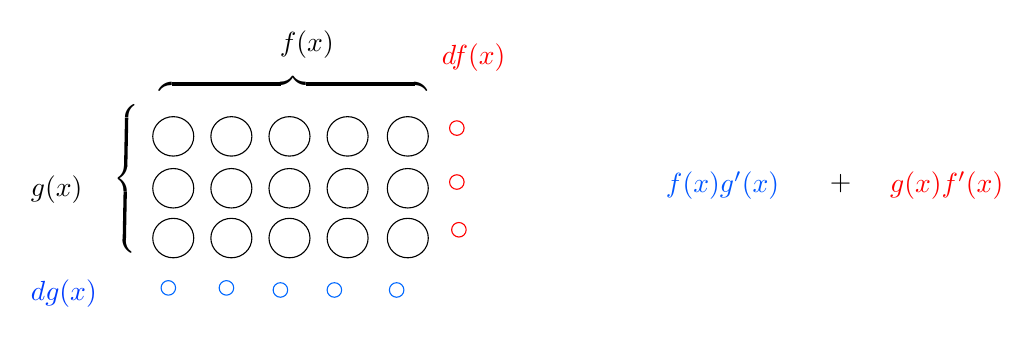
\begin{tikzpicture}[x=0.75pt,y=0.75pt,yscale=-1,xscale=1]
%uncomment if require: \path (0,300); %set diagram left start at 0, and has height of 300

%Shape: Ellipse [id:dp06031973450750061] 
\draw   (164,126.5) .. controls (164,121.25) and (168.42,117) .. (173.88,117) .. controls (179.33,117) and (183.75,121.25) .. (183.75,126.5) .. controls (183.75,131.75) and (179.33,136) .. (173.88,136) .. controls (168.42,136) and (164,131.75) .. (164,126.5) -- cycle ;
%Shape: Ellipse [id:dp8478408655553544] 
\draw   (192,126.5) .. controls (192,121.25) and (196.42,117) .. (201.88,117) .. controls (207.33,117) and (211.75,121.25) .. (211.75,126.5) .. controls (211.75,131.75) and (207.33,136) .. (201.88,136) .. controls (196.42,136) and (192,131.75) .. (192,126.5) -- cycle ;
%Shape: Ellipse [id:dp505421117341947] 
\draw   (220,126.5) .. controls (220,121.25) and (224.42,117) .. (229.88,117) .. controls (235.33,117) and (239.75,121.25) .. (239.75,126.5) .. controls (239.75,131.75) and (235.33,136) .. (229.88,136) .. controls (224.42,136) and (220,131.75) .. (220,126.5) -- cycle ;
%Shape: Ellipse [id:dp007218742660141997] 
\draw   (248,126.5) .. controls (248,121.25) and (252.42,117) .. (257.88,117) .. controls (263.33,117) and (267.75,121.25) .. (267.75,126.5) .. controls (267.75,131.75) and (263.33,136) .. (257.88,136) .. controls (252.42,136) and (248,131.75) .. (248,126.5) -- cycle ;
%Shape: Ellipse [id:dp8702465733669611] 
\draw   (277,126.5) .. controls (277,121.25) and (281.42,117) .. (286.88,117) .. controls (292.33,117) and (296.75,121.25) .. (296.75,126.5) .. controls (296.75,131.75) and (292.33,136) .. (286.88,136) .. controls (281.42,136) and (277,131.75) .. (277,126.5) -- cycle ;
%Shape: Ellipse [id:dp6716570870833466] 
\draw   (164,151.5) .. controls (164,146.25) and (168.42,142) .. (173.88,142) .. controls (179.33,142) and (183.75,146.25) .. (183.75,151.5) .. controls (183.75,156.75) and (179.33,161) .. (173.88,161) .. controls (168.42,161) and (164,156.75) .. (164,151.5) -- cycle ;
%Shape: Ellipse [id:dp1820921953890161] 
\draw   (192,151.5) .. controls (192,146.25) and (196.42,142) .. (201.88,142) .. controls (207.33,142) and (211.75,146.25) .. (211.75,151.5) .. controls (211.75,156.75) and (207.33,161) .. (201.88,161) .. controls (196.42,161) and (192,156.75) .. (192,151.5) -- cycle ;
%Shape: Ellipse [id:dp5866793827026061] 
\draw   (220,151.5) .. controls (220,146.25) and (224.42,142) .. (229.88,142) .. controls (235.33,142) and (239.75,146.25) .. (239.75,151.5) .. controls (239.75,156.75) and (235.33,161) .. (229.88,161) .. controls (224.42,161) and (220,156.75) .. (220,151.5) -- cycle ;
%Shape: Ellipse [id:dp45797332679454195] 
\draw   (248,151.5) .. controls (248,146.25) and (252.42,142) .. (257.88,142) .. controls (263.33,142) and (267.75,146.25) .. (267.75,151.5) .. controls (267.75,156.75) and (263.33,161) .. (257.88,161) .. controls (252.42,161) and (248,156.75) .. (248,151.5) -- cycle ;
%Shape: Ellipse [id:dp24430516488734677] 
\draw   (277,151.5) .. controls (277,146.25) and (281.42,142) .. (286.88,142) .. controls (292.33,142) and (296.75,146.25) .. (296.75,151.5) .. controls (296.75,156.75) and (292.33,161) .. (286.88,161) .. controls (281.42,161) and (277,156.75) .. (277,151.5) -- cycle ;
%Shape: Ellipse [id:dp5662108764983852] 
\draw   (164,175.5) .. controls (164,170.25) and (168.42,166) .. (173.88,166) .. controls (179.33,166) and (183.75,170.25) .. (183.75,175.5) .. controls (183.75,180.75) and (179.33,185) .. (173.88,185) .. controls (168.42,185) and (164,180.75) .. (164,175.5) -- cycle ;
%Shape: Ellipse [id:dp6579543801408282] 
\draw   (192,175.5) .. controls (192,170.25) and (196.42,166) .. (201.88,166) .. controls (207.33,166) and (211.75,170.25) .. (211.75,175.5) .. controls (211.75,180.75) and (207.33,185) .. (201.88,185) .. controls (196.42,185) and (192,180.75) .. (192,175.5) -- cycle ;
%Shape: Ellipse [id:dp17883475704623442] 
\draw   (220,175.5) .. controls (220,170.25) and (224.42,166) .. (229.88,166) .. controls (235.33,166) and (239.75,170.25) .. (239.75,175.5) .. controls (239.75,180.75) and (235.33,185) .. (229.88,185) .. controls (224.42,185) and (220,180.75) .. (220,175.5) -- cycle ;
%Shape: Ellipse [id:dp8959152379599131] 
\draw   (248,175.5) .. controls (248,170.25) and (252.42,166) .. (257.88,166) .. controls (263.33,166) and (267.75,170.25) .. (267.75,175.5) .. controls (267.75,180.75) and (263.33,185) .. (257.88,185) .. controls (252.42,185) and (248,180.75) .. (248,175.5) -- cycle ;
%Shape: Ellipse [id:dp8976107913184502] 
\draw   (277,175.5) .. controls (277,170.25) and (281.42,166) .. (286.88,166) .. controls (292.33,166) and (296.75,170.25) .. (296.75,175.5) .. controls (296.75,180.75) and (292.33,185) .. (286.88,185) .. controls (281.42,185) and (277,180.75) .. (277,175.5) -- cycle ;
%Shape: Circle [id:dp01856382719091243] 
\draw  [color={rgb, 255:red, 255; green, 0; blue, 0 }  ,draw opacity=1 ] (307,122.5) .. controls (307,120.57) and (308.57,119) .. (310.5,119) .. controls (312.43,119) and (314,120.57) .. (314,122.5) .. controls (314,124.43) and (312.43,126) .. (310.5,126) .. controls (308.57,126) and (307,124.43) .. (307,122.5) -- cycle ;
%Shape: Circle [id:dp4403664682847295] 
\draw  [color={rgb, 255:red, 0; green, 104; blue, 255 }  ,draw opacity=1 ] (168,199.5) .. controls (168,197.57) and (169.57,196) .. (171.5,196) .. controls (173.43,196) and (175,197.57) .. (175,199.5) .. controls (175,201.43) and (173.43,203) .. (171.5,203) .. controls (169.57,203) and (168,201.43) .. (168,199.5) -- cycle ;
%Shape: Circle [id:dp07179694909069678] 
\draw  [color={rgb, 255:red, 0; green, 104; blue, 255 }  ,draw opacity=1 ] (196,199.5) .. controls (196,197.57) and (197.57,196) .. (199.5,196) .. controls (201.43,196) and (203,197.57) .. (203,199.5) .. controls (203,201.43) and (201.43,203) .. (199.5,203) .. controls (197.57,203) and (196,201.43) .. (196,199.5) -- cycle ;
%Shape: Circle [id:dp1451673451815234] 
\draw  [color={rgb, 255:red, 0; green, 104; blue, 255 }  ,draw opacity=1 ] (222,200.5) .. controls (222,198.57) and (223.57,197) .. (225.5,197) .. controls (227.43,197) and (229,198.57) .. (229,200.5) .. controls (229,202.43) and (227.43,204) .. (225.5,204) .. controls (223.57,204) and (222,202.43) .. (222,200.5) -- cycle ;
%Shape: Circle [id:dp9161876920152885] 
\draw  [color={rgb, 255:red, 0; green, 104; blue, 255 }  ,draw opacity=1 ] (248,200.5) .. controls (248,198.57) and (249.57,197) .. (251.5,197) .. controls (253.43,197) and (255,198.57) .. (255,200.5) .. controls (255,202.43) and (253.43,204) .. (251.5,204) .. controls (249.57,204) and (248,202.43) .. (248,200.5) -- cycle ;
%Shape: Circle [id:dp7144565199430419] 
\draw  [color={rgb, 255:red, 0; green, 104; blue, 255 }  ,draw opacity=1 ] (278,200.5) .. controls (278,198.57) and (279.57,197) .. (281.5,197) .. controls (283.43,197) and (285,198.57) .. (285,200.5) .. controls (285,202.43) and (283.43,204) .. (281.5,204) .. controls (279.57,204) and (278,202.43) .. (278,200.5) -- cycle ;
%Shape: Circle [id:dp8377649456481785] 
\draw  [color={rgb, 255:red, 255; green, 0; blue, 0 }  ,draw opacity=1 ] (307,148.5) .. controls (307,146.57) and (308.57,145) .. (310.5,145) .. controls (312.43,145) and (314,146.57) .. (314,148.5) .. controls (314,150.43) and (312.43,152) .. (310.5,152) .. controls (308.57,152) and (307,150.43) .. (307,148.5) -- cycle ;
%Shape: Circle [id:dp940388133671272] 
\draw  [color={rgb, 255:red, 255; green, 0; blue, 0 }  ,draw opacity=1 ] (308,171.5) .. controls (308,169.57) and (309.57,168) .. (311.5,168) .. controls (313.43,168) and (315,169.57) .. (315,171.5) .. controls (315,173.43) and (313.43,175) .. (311.5,175) .. controls (309.57,175) and (308,173.43) .. (308,171.5) -- cycle ;

% Text Node
\draw (224,74.4) node [anchor=north west][inner sep=0.75pt]    {$f( x)$};
% Text Node
\draw (166,96.4) node [anchor=north west][inner sep=0.75pt]    {$\overbrace{\ \ \ \ \ \ \ \ \ \ \ \ \ \ \ \ \ \ \ \ \ \ \ \ \ \ \ \ \ }$};
% Text Node
\draw (145.21,183.74) node [anchor=north west][inner sep=0.75pt]  [rotate=-271.09]  {$\overbrace{\ \ \ \ \ \ \ \ \ \ \ \ \ \ \ \ }$};
% Text Node
\draw (104,144.4) node [anchor=north west][inner sep=0.75pt]    {$g( x)$};
% Text Node
\draw (302,80.4) node [anchor=north west][inner sep=0.75pt]  [color={rgb, 255:red, 255; green, 0; blue, 0 }  ,opacity=1 ]  {$df( x)$};
% Text Node
\draw (104,194.4) node [anchor=north west][inner sep=0.75pt]  [color={rgb, 255:red, 0; green, 59; blue, 255 }  ,opacity=1 ]  {$dg( x)$};
% Text Node
\draw (410,142.4) node [anchor=north west][inner sep=0.75pt]  [color={rgb, 255:red, 0; green, 86; blue, 255 }  ,opacity=1 ]  {$f( x) g'( x)$};
% Text Node
\draw (489,143.4) node [anchor=north west][inner sep=0.75pt]    {$+$};
% Text Node
\draw (518,142.4) node [anchor=north west][inner sep=0.75pt]  [color={rgb, 255:red, 255; green, 0; blue, 0 }  ,opacity=1 ]  {$g( x) f'( x)$};


\end{tikzpicture}

\subsubsection{Chain}

We run through \( f \) at a rate specified by \( g \).
Thus if we want to convert \( dx \) to \( \dv{f}{x} \)
but we only know \( \dv{f}{g} \),
we just have to multiply by the change in rate of \( g \)

\tikzset{every picture/.style={line width=0.75pt}} %set default line width to 0.75pt        
\noindent
\begin{tikzpicture}[x=0.75pt,y=0.75pt,yscale=-1,xscale=1]
%uncomment if require: \path (0,300); %set diagram left start at 0, and has height of 300

%Shape: Axis 2D [id:dp3419332376667883] 
\draw  (41,249) -- (334.5,249)(78.73,15) -- (78.73,274) (327.5,244) -- (334.5,249) -- (327.5,254) (73.73,22) -- (78.73,15) -- (83.73,22) (127.73,244) -- (127.73,254)(176.73,244) -- (176.73,254)(225.73,244) -- (225.73,254)(274.73,244) -- (274.73,254)(73.73,200) -- (83.73,200)(73.73,151) -- (83.73,151)(73.73,102) -- (83.73,102)(73.73,53) -- (83.73,53) ;
\draw   ;
%Shape: Circle [id:dp15714841919076528] 
\draw   (278,132.75) .. controls (278,129.57) and (280.57,127) .. (283.75,127) .. controls (286.93,127) and (289.5,129.57) .. (289.5,132.75) .. controls (289.5,135.93) and (286.93,138.5) .. (283.75,138.5) .. controls (280.57,138.5) and (278,135.93) .. (278,132.75) -- cycle ;
%Curve Lines [id:da48902714333738084] 
\draw    (79,183) .. controls (88.79,175.66) and (92.03,119.89) .. (120.27,166.95) .. controls (148.5,214) and (187.02,172.39) .. (223.5,199) .. controls (259.98,225.61) and (248.5,129) .. (278,132.75) ;
%Straight Lines [id:da8141145633432557] 
\draw [color={rgb, 255:red, 255; green, 0; blue, 0 }  ,draw opacity=1 ]   (283,115) -- (283,74) ;
\draw [shift={(283,72)}, rotate = 450] [color={rgb, 255:red, 255; green, 0; blue, 0 }  ,draw opacity=1 ][line width=0.75]    (10.93,-3.29) .. controls (6.95,-1.4) and (3.31,-0.3) .. (0,0) .. controls (3.31,0.3) and (6.95,1.4) .. (10.93,3.29)   ;
%Straight Lines [id:da3154003786291655] 
\draw [color={rgb, 255:red, 255; green, 0; blue, 0 }  ,draw opacity=1 ]   (282.75,148.5) -- (282.75,187) ;
\draw [shift={(282.75,189)}, rotate = 270] [color={rgb, 255:red, 255; green, 0; blue, 0 }  ,draw opacity=1 ][line width=0.75]    (10.93,-3.29) .. controls (6.95,-1.4) and (3.31,-0.3) .. (0,0) .. controls (3.31,0.3) and (6.95,1.4) .. (10.93,3.29)   ;
%Straight Lines [id:da19276906577043762] 
\draw  [dash pattern={on 0.84pt off 2.51pt}]  (283.75,138.5) -- (283.75,257) ;
%Straight Lines [id:da9895246969397727] 
\draw [color={rgb, 255:red, 0; green, 42; blue, 255 }  ,draw opacity=1 ]   (248,272) -- (279.5,272) ;
\draw [shift={(281.5,272)}, rotate = 180] [color={rgb, 255:red, 0; green, 42; blue, 255 }  ,draw opacity=1 ][line width=0.75]    (10.93,-3.29) .. controls (6.95,-1.4) and (3.31,-0.3) .. (0,0) .. controls (3.31,0.3) and (6.95,1.4) .. (10.93,3.29)   ;
%Shape: Axis 2D [id:dp074444405148542] 
\draw  (338,248) -- (631.5,248)(375.73,14) -- (375.73,273) (624.5,243) -- (631.5,248) -- (624.5,253) (370.73,21) -- (375.73,14) -- (380.73,21) (424.73,243) -- (424.73,253)(473.73,243) -- (473.73,253)(522.73,243) -- (522.73,253)(571.73,243) -- (571.73,253)(370.73,199) -- (380.73,199)(370.73,150) -- (380.73,150)(370.73,101) -- (380.73,101)(370.73,52) -- (380.73,52) ;
\draw   ;
%Shape: Circle [id:dp6593224815387302] 
\draw   (575,131.75) .. controls (575,128.57) and (577.57,126) .. (580.75,126) .. controls (583.93,126) and (586.5,128.57) .. (586.5,131.75) .. controls (586.5,134.93) and (583.93,137.5) .. (580.75,137.5) .. controls (577.57,137.5) and (575,134.93) .. (575,131.75) -- cycle ;
%Curve Lines [id:da4000391883296601] 
\draw    (376,182) .. controls (385.79,174.66) and (412.27,121.95) .. (440.5,169) .. controls (468.73,216.05) and (458.02,173.39) .. (494.5,200) .. controls (530.98,226.61) and (540.5,199) .. (575,131.75) ;
%Straight Lines [id:da6430080624749632] 
\draw [color={rgb, 255:red, 255; green, 0; blue, 0 }  ,draw opacity=1 ]   (580,114) -- (580,73) ;
\draw [shift={(580,71)}, rotate = 450] [color={rgb, 255:red, 255; green, 0; blue, 0 }  ,draw opacity=1 ][line width=0.75]    (10.93,-3.29) .. controls (6.95,-1.4) and (3.31,-0.3) .. (0,0) .. controls (3.31,0.3) and (6.95,1.4) .. (10.93,3.29)   ;
%Straight Lines [id:da3118969368266129] 
\draw [color={rgb, 255:red, 255; green, 0; blue, 0 }  ,draw opacity=1 ]   (579.75,147.5) -- (579.75,186) ;
\draw [shift={(579.75,188)}, rotate = 270] [color={rgb, 255:red, 255; green, 0; blue, 0 }  ,draw opacity=1 ][line width=0.75]    (10.93,-3.29) .. controls (6.95,-1.4) and (3.31,-0.3) .. (0,0) .. controls (3.31,0.3) and (6.95,1.4) .. (10.93,3.29)   ;
%Straight Lines [id:da9742164918890941] 
\draw  [dash pattern={on 0.84pt off 2.51pt}]  (580.75,137.5) -- (580.75,256) ;
%Straight Lines [id:da590167212523919] 
\draw [color={rgb, 255:red, 0; green, 42; blue, 255 }  ,draw opacity=1 ]   (545,271) -- (576.5,271) ;
\draw [shift={(578.5,271)}, rotate = 180] [color={rgb, 255:red, 0; green, 42; blue, 255 }  ,draw opacity=1 ][line width=0.75]    (10.93,-3.29) .. controls (6.95,-1.4) and (3.31,-0.3) .. (0,0) .. controls (3.31,0.3) and (6.95,1.4) .. (10.93,3.29)   ;

% Text Node
\draw (35,124.4) node [anchor=north west][inner sep=0.75pt]    {$f$};
% Text Node
\draw (168,261.4) node [anchor=north west][inner sep=0.75pt]    {$g$};
% Text Node
\draw (332,123.4) node [anchor=north west][inner sep=0.75pt]    {$f$};
% Text Node
\draw (468,263.4) node [anchor=north west][inner sep=0.75pt]    {$x$};
% Text Node
\draw (547,274.4) node [anchor=north west][inner sep=0.75pt]    {$g( x)$};


\end{tikzpicture}

\( \dv{x} f(g) = f'(g)g' \)

\subsubsection{Reciprocol}

\( \dv{x} \frac{1}{x} = - \frac{1}{x} \cdot \frac{1}{x} = - \frac{1}{x^2} \)


\tikzset{every picture/.style={line width=0.75pt}} %set default line width to 0.75pt        
\noindent
\begin{tikzpicture}[x=0.75pt,y=0.75pt,yscale=-1,xscale=1]
%uncomment if require: \path (0,300); %set diagram left start at 0, and has height of 300

%Straight Lines [id:da21843410649174944] 
\draw    (26,152) -- (277.5,152) ;
\draw [shift={(277.5,152)}, rotate = 180] [color={rgb, 255:red, 0; green, 0; blue, 0 }  ][line width=0.75]    (0,5.59) -- (0,-5.59)   ;
\draw [shift={(26,152)}, rotate = 180] [color={rgb, 255:red, 0; green, 0; blue, 0 }  ][line width=0.75]    (0,5.59) -- (0,-5.59)   ;
%Shape: Rectangle [id:dp4515994731638744] 
\draw  [color={rgb, 255:red, 255; green, 0; blue, 0 }  ,draw opacity=1 ] (26,105) -- (149.5,105) -- (149.5,133) -- (26,133) -- cycle ;
%Shape: Brace [id:dp08423244109966566] 
\draw  [color={rgb, 255:red, 0; green, 0; blue, 0 }  ,draw opacity=1 ] (26.91,206.38) .. controls (26.91,211.05) and (29.24,213.38) .. (33.91,213.38) -- (141.75,213.38) .. controls (148.42,213.38) and (151.75,215.71) .. (151.75,220.38) .. controls (151.75,215.71) and (155.08,213.38) .. (161.75,213.38)(158.75,213.38) -- (269.59,213.38) .. controls (274.26,213.38) and (276.59,211.05) .. (276.59,206.38) ;
%Shape: Brace [id:dp03278570786281365] 
\draw  [color={rgb, 255:red, 255; green, 0; blue, 4 }  ,draw opacity=1 ] (149,88) .. controls (149,83.33) and (146.67,81) .. (142,81) -- (98.25,81) .. controls (91.58,81) and (88.25,78.67) .. (88.25,74) .. controls (88.25,78.67) and (84.92,81) .. (78.25,81)(81.25,81) -- (34.5,81) .. controls (29.83,81) and (27.5,83.33) .. (27.5,88) ;
%Shape: Brace [id:dp9522391936570531] 
\draw  [color={rgb, 255:red, 0; green, 59; blue, 255 }  ,draw opacity=1 ] (27.5,167) .. controls (27.5,171.67) and (29.83,174) .. (34.5,174) -- (78,174) .. controls (84.67,174) and (88,176.33) .. (88,181) .. controls (88,176.33) and (91.33,174) .. (98,174)(95,174) -- (141.5,174) .. controls (146.17,174) and (148.5,171.67) .. (148.5,167) ;
%Straight Lines [id:da4718568555643836] 
\draw    (348,150) -- (599.5,150) ;
\draw [shift={(348,150)}, rotate = 180] [color={rgb, 255:red, 0; green, 0; blue, 0 }  ][line width=0.75]    (0,5.59) -- (0,-5.59)   ;
%Shape: Rectangle [id:dp8513478800250758] 
\draw  [color={rgb, 255:red, 255; green, 0; blue, 0 }  ,draw opacity=1 ] (348,103) -- (471.5,103) -- (471.5,131) -- (348,131) -- cycle ;
%Shape: Brace [id:dp17739490270334712] 
\draw  [color={rgb, 255:red, 0; green, 0; blue, 0 }  ,draw opacity=1 ] (348.91,204.38) .. controls (348.91,209.05) and (351.24,211.38) .. (355.91,211.38) -- (463.75,211.38) .. controls (470.42,211.38) and (473.75,213.71) .. (473.75,218.38) .. controls (473.75,213.71) and (477.08,211.38) .. (483.75,211.38)(480.75,211.38) -- (591.59,211.38) .. controls (596.26,211.38) and (598.59,209.05) .. (598.59,204.38) ;
%Shape: Brace [id:dp9740788101727171] 
\draw  [color={rgb, 255:red, 255; green, 0; blue, 4 }  ,draw opacity=1 ] (471,86) .. controls (471,81.33) and (468.67,79) .. (464,79) -- (420.25,79) .. controls (413.58,79) and (410.25,76.67) .. (410.25,72) .. controls (410.25,76.67) and (406.92,79) .. (400.25,79)(403.25,79) -- (356.5,79) .. controls (351.83,79) and (349.5,81.33) .. (349.5,86) ;
%Shape: Brace [id:dp5640321305233592] 
\draw  [color={rgb, 255:red, 0; green, 59; blue, 255 }  ,draw opacity=1 ] (349.5,165) .. controls (349.5,169.67) and (351.83,172) .. (356.5,172) -- (400,172) .. controls (406.67,172) and (410,174.33) .. (410,179) .. controls (410,174.33) and (413.33,172) .. (420,172)(417,172) -- (463.5,172) .. controls (468.17,172) and (470.5,169.67) .. (470.5,165) ;
%Shape: Brace [id:dp5650547309026009] 
\draw  [color={rgb, 255:red, 255; green, 0; blue, 0 }  ,draw opacity=1 ] (599.91,206.38) .. controls (599.91,209.89) and (601.67,211.65) .. (605.18,211.65) -- (605.18,211.65) .. controls (610.19,211.65) and (612.7,213.41) .. (612.7,216.92) .. controls (612.7,213.41) and (615.21,211.65) .. (620.23,211.65)(617.97,211.65) -- (620.23,211.65) .. controls (623.74,211.65) and (625.5,209.89) .. (625.5,206.38) ;
%Straight Lines [id:da6965968095386313] 
\draw [color={rgb, 255:red, 255; green, 0; blue, 4 }  ,draw opacity=1 ]   (599.5,150) -- (622.5,150)  ;
\draw [shift={(622.5,150)}, rotate = 180] [color={rgb, 255:red, 255; green, 0; blue, 4 }  ,draw opacity=1 ][line width=0.75]    (0,5.59) -- (0,-5.59)   ;

% Text Node
\draw (144,230.4) node [anchor=north west][inner sep=0.75pt]    {$x$};
% Text Node
\draw (83,48.4) node [anchor=north west][inner sep=0.75pt]  [color={rgb, 255:red, 255; green, 0; blue, 0 }  ,opacity=1 ]  {$1$};
% Text Node
\draw (75,186.4) node [anchor=north west][inner sep=0.75pt]  [color={rgb, 255:red, 0; green, 42; blue, 255 }  ,opacity=1 ]  {$1/x$};
% Text Node
\draw (466,228.4) node [anchor=north west][inner sep=0.75pt]    {$x$};
% Text Node
\draw (405,46.4) node [anchor=north west][inner sep=0.75pt]  [color={rgb, 255:red, 255; green, 0; blue, 0 }  ,opacity=1 ]  {$1$};
% Text Node
\draw (374,185.4) node [anchor=north west][inner sep=0.75pt]  [color={rgb, 255:red, 0; green, 42; blue, 255 }  ,opacity=1 ]  {$1/( x+dx)$};
% Text Node
\draw (605,226.4) node [anchor=north west][inner sep=0.75pt]  [color={rgb, 255:red, 255; green, 0; blue, 0 }  ,opacity=1 ]  {$dx$};


\end{tikzpicture}

\subsubsection{Quotient}

\( \dv{x} fg^{-1} = f'g^{-1} - fg^{-2}g' = \frac{f'g - fg'}{g^2} \)

\subsubsection{exp and log}

We know \( \dv{x} b^x = ab^x \) where \( a \) is some proportion.
We also know that \( b^x = e^{\ln(b) x} \) so
\[ \dv{x} b^x = b^x \dv{x} \ln(b) x = b^x \ln(b) \]
Thus \( a = \ln(b) \).

At some proportion \( e^x \), our rate of growth is \( e^x \).
If we take the inverse \( \ln(x) \), then instead of multiplying, we divide.
so \( \dv{x} \ln(x) = \frac{1}{x} \).

\subsubsection{Inverse}


\end{document}
